\documentclass[11pt,a4paper,oneside]{report}
\usepackage{fontspec}
\setmainfont{Cambria}
\setsansfont{Segoe UI}
\setmonofont{Consolas}[Scale=0.9]
\usepackage[spanish,es-noshorthands]{babel}
\usepackage[margin=2.3cm,headheight=15pt]{geometry}
\usepackage[table]{xcolor}
\usepackage{xltabular}
\usepackage{array}
\usepackage{enumitem}
\usepackage{fancyhdr}
\usepackage{titlesec}
\usepackage{graphicx}
\usepackage{float}
\usepackage{caption}
\usepackage{listings}
\usepackage[most]{tcolorbox}
\usepackage[hidelinks]{hyperref}

% Paleta de SIDEM (la misma de la aplicación y de la presentación)
\definecolor{azul}{HTML}{2563EB}
\definecolor{tinta}{HTML}{1E293B}
\definecolor{gris}{HTML}{64748B}
\definecolor{borde}{HTML}{CBD5E1}
\definecolor{fondo}{HTML}{F0F4F8}
\definecolor{cabecera}{HTML}{E2E8F0}
\definecolor{verde}{HTML}{16A34A}
\definecolor{ambar}{HTML}{D97706}
\definecolor{rojo}{HTML}{DC2626}
\arrayrulecolor{borde}

\hypersetup{pdftitle={Informe final de pruebas - SIDEM},pdfauthor={Equipo SIDEM}}

\pagestyle{fancy}
\fancyhf{}
\fancyhead[L]{\color{gris}\sffamily\small Informe final de pruebas · SIDEM}
\fancyhead[R]{\color{gris}\sffamily\small ISO/IEC/IEEE 29119-3}
\fancyfoot[C]{\color{gris}\sffamily\small\thepage}
\renewcommand{\headrulewidth}{0.4pt}
\fancypagestyle{plain}{\fancyhf{}\fancyfoot[C]{\color{gris}\sffamily\small\thepage}\renewcommand{\headrulewidth}{0pt}}

\titleformat{\part}[display]{\centering\sffamily\color{azul}}{}{0pt}{\Huge\bfseries}
\titleformat{\chapter}[block]{\sffamily\color{tinta}\huge\bfseries}{}{0pt}{}[\vspace{2pt}{\color{azul}\titlerule[1.2pt]}]
\titleformat{\section}{\sffamily\color{azul}\Large\bfseries}{}{0pt}{}
\titleformat{\subsection}{\sffamily\color{tinta}\large\bfseries}{}{0pt}{}
\titleformat{\subsubsection}{\sffamily\color{tinta}\normalsize\bfseries}{}{0pt}{}
\titlespacing*{\chapter}{0pt}{0pt}{14pt}
\titlespacing*{\section}{0pt}{14pt}{5pt}
\titlespacing*{\subsection}{0pt}{10pt}{4pt}

\setlist[itemize]{leftmargin=1.3em,itemsep=2pt,topsep=3pt}
\setlist[enumerate]{leftmargin=1.6em,itemsep=2pt,topsep=3pt}
\setlength{\parindent}{0pt}
\setlength{\parskip}{5pt}
\renewcommand{\arraystretch}{1.35}
\captionsetup{font={small,sf},labelfont={bf,color=azul}}

\newcommand{\code}[1]{{\ttfamily\color{tinta}#1}}
\newtcolorbox{nota}{enhanced,breakable,colback=fondo,colframe=azul,boxrule=0pt,leftrule=2.5pt,arc=0pt,
  left=8pt,right=8pt,top=4pt,bottom=4pt,before skip=6pt,after skip=6pt}
\lstset{basicstyle=\ttfamily\footnotesize,breaklines=true,columns=fullflexible,keepspaces=true,
  backgroundcolor=\color{fondo},frame=single,rulecolor=\color{borde},xleftmargin=4pt,xrightmargin=4pt,
  framesep=5pt,upquote=true,extendedchars=true}
\setcounter{tocdepth}{1}
\setlength{\emergencystretch}{3em}


\begin{document}


\begin{titlepage}
\sffamily
\vspace*{1.2cm}
{\color{verde}\rule{0.9cm}{0.9cm}}\hspace{6pt}{\color{ambar}\rule{0.9cm}{0.9cm}}\hspace{6pt}{\color{rojo}\rule{0.9cm}{0.9cm}}\par
\vspace{1.4cm}
{\color{azul}\large\bfseries PRUEBAS DE SOFTWARE 2026-2 · ISO/IEC/IEEE 29119-3}\par
\vspace{0.4cm}
{\color{tinta}\fontsize{32}{38}\selectfont\bfseries Informe final de pruebas\\[4pt] de SIDEM}\par
\vspace{0.5cm}
{\color{gris}\Large Plan, ejecución, defectos, correcciones y cierre}\par
\vspace{0.3cm}
{\color{gris}\large Sistema de seguimiento a docentes en Moodle}\par
\vfill
{\color{tinta}\large\bfseries Equipo}\par\vspace{4pt}
{\color{tinta}\large Marcos Duque Jaramillo\\ Sebastián Díaz Jiménez\\ Nicolás Cataño Durango\\ Julián Ramírez Molina}\par
\vspace{0.8cm}
{\color{tinta}\large\bfseries Docente}\par\vspace{4pt}
{\color{tinta}\large Roberto José Calderón Bermejo}\par
\vspace{0.8cm}
{\color{gris}17 de noviembre de 2026 · Repositorio: \href{https://github.com/C4t-eyex/SIDEM-Plan-Pruebas}{github.com/C4t-eyex/SIDEM-Plan-Pruebas}}\par
\end{titlepage}


\tableofcontents\clearpage


\chapter*{Introducción}\addcontentsline{toc}{chapter}{Introducción}
Este informe reúne el trabajo final del curso: un plan de pruebas según la norma ISO/IEC/IEEE 29119-3, adaptado (\emph{tailoring}) a un ciclo de 9 días, y su ejecución sobre SIDEM, el sistema de seguimiento a docentes en Moodle. Se probó la versión \code{77f71b2} en una demo con Docker y datos ficticios, sin usar la base de producción.

\begin{nota}
\textbf{Resultado.} Los 9 casos planeados (TC-01 a TC-09) se ejecutaron. La primera ronda de pruebas automáticas dio 16 de 19 y encontró, junto con la ejecución manual y el montaje de la demo, 5 defectos (1 alto, 2 medios y 2 bajos). Los 5 se corrigieron con parches sobre la versión probada y en el retest del 16/11/2026 pasan las 19 pruebas. Se cumplen todos los criterios de finalización del plan.
\end{nota}

\textbf{Cómo está organizado.}
\begin{itemize}
\item \textbf{Parte I. Plan de pruebas:} el plan completo en las 8 secciones pedidas (versión 1.0).
\item \textbf{Parte II. Ejecución:} las hojas de ejecución manual con lo obtenido, las pruebas automáticas y el índice de evidencias.
\item \textbf{Parte III. Defectos, correcciones y retest:} el registro de defectos, la evidencia visual del antes y el después, las correcciones y el retest.
\item \textbf{Parte IV. Informe de cierre:} el \emph{Test Completion Report} (versión 1.0).
\item \textbf{Anexos:} preguntas al docente, bitácora de avances y antecedentes (Actividades 1 y 2, matriz de riesgos y Talleres 4 y 5).
\end{itemize}

Todo el material, incluidas las capturas, las salidas de pytest y los parches, está en el repositorio del equipo. Las rutas de archivo que aparecen en el texto son rutas dentro de ese repositorio.


\part*{Parte I. Plan de pruebas}


\chapter*{Plan de pruebas}\addcontentsline{toc}{chapter}{Plan de pruebas}

\begin{nota}
Basado en la norma ISO/IEC/IEEE 29119-3 (Documentación de pruebas), adaptada a un ciclo corto de 9 días (09/11/2026 al 17/11/2026). \textbf{Estado:} versión 1.0, final - ciclo ejecutado y cerrado (ver \code{informe-\allowbreak{}de-\allowbreak{}cierre.\allowbreak{}md}).

\end{nota}

\section*{1. Información específica del documento}\addcontentsline{toc}{section}{1. Información específica del documento}

\subsection*{1.1 Identificador único del documento}\addcontentsline{toc}{subsection}{1.1 Identificador único del documento}

\code{SIDEM-\allowbreak{}PP-\allowbreak{}2026-\allowbreak{}01} (Plan de Pruebas, versión 1.0)


\subsection*{1.2 Organización emisora y autores}\addcontentsline{toc}{subsection}{1.2 Organización emisora y autores}

\begin{itemize}
\item \textbf{Organización:} Equipo SIDEM - curso Pruebas de Software, 2026-2.
\item \textbf{Autores:} Marcos Duque Jaramillo, Sebastián Díaz Jiménez, Nicolás Cataño Durango, Julián Ramírez Molina.
\end{itemize}

\subsection*{1.3 Autoridad de aprobación}\addcontentsline{toc}{subsection}{1.3 Autoridad de aprobación}

Roberto José Calderón Bermejo, docente del curso de Pruebas de Software.


\subsection*{1.4 Historial de cambios y control de versiones}\addcontentsline{toc}{subsection}{1.4 Historial de cambios y control de versiones}

{\small
\begin{xltabular}{\linewidth}{>{\hsize=0.428\hsize\raggedright\arraybackslash}X>{\hsize=0.475\hsize\raggedright\arraybackslash}X>{\hsize=0.428\hsize\raggedright\arraybackslash}X>{\hsize=2.669\hsize\raggedright\arraybackslash}X}
\hline\rowcolor{cabecera}
\textbf{Versión} & \textbf{Fecha} & \textbf{Autor} & \textbf{Cambio} \\ \hline
\endhead
0.1 & 08/11/2026 & Equipo SIDEM & Primer borrador: consolida Actividades 1 y 2, matriz de riesgos y Talleres 4 y 5. \\ \hline
0.2 & 08/11/2026 & Equipo SIDEM & Ajuste de TC-01, TC-03 y DAT-01 según el funcionamiento real de SIDEM, revisado al montar la demo. \\ \hline
0.3 & 08/11/2026 & Equipo SIDEM & DAT-01 con revisión 2 y zona horaria de la base; complemento automático de TC-06. \\ \hline
0.4 & 10/11/2026 & Equipo SIDEM & Casos identificados no ejecutados TC-10 a TC-17 (dos por integrante), según indicación del docente. \\ \hline
0.5 & 10/11/2026 & Equipo SIDEM & Cronograma ajustado a la exposición del 17/11/2026, según indicación del docente. \\ \hline
0.6 & 16/11/2026 & Equipo SIDEM & Respuestas del docente incorporadas (\code{preguntas-\allowbreak{}para-\allowbreak{}el-\allowbreak{}profe.\allowbreak{}md}): escala 1-3 válida, R10 fuera del alcance del equipo, entrega final en PDF. \\ \hline
1.0 & 17/11/2026 & Equipo SIDEM & Versión final: ciclo ejecutado, retest del 16/11 con los 5 defectos cerrados y criterios de finalización cumplidos (\code{informe-\allowbreak{}de-\allowbreak{}cierre.\allowbreak{}md}). \\ \hline
\end{xltabular}}


El control de versiones del documento se lleva en este repositorio (historial de commits de Git).


\section*{2. Introducción y declaración de adaptación (Tailoring)}\addcontentsline{toc}{section}{2. Introducción y declaración de adaptación (Tailoring)}

\subsection*{2.1 Alcance del documento}\addcontentsline{toc}{subsection}{2.1 Alcance del documento}

Este plan define qué se va a probar de SIDEM, por qué, cómo, con qué recursos y en qué tiempo. Cubre las pruebas funcionales, de control de acceso por roles y de confiabilidad de las métricas del \textbf{seguimiento a docentes}.


\textbf{Sistema bajo prueba.} SIDEM (Sistema de Seguimiento de Docentes en Moodle) es una aplicación web en Python (FastAPI) con base de datos PostgreSQL. Permite a los revisores evaluar criterios de acompañamiento docente por curso y por revisión del semestre. Además, muestra a los líderes académicos un semáforo de cumplimiento y un panel de métricas.


\subsection*{2.2 Referencias documentales}\addcontentsline{toc}{subsection}{2.2 Referencias documentales}

{\small
\begin{xltabular}{\linewidth}{>{\hsize=0.402\hsize\raggedright\arraybackslash}X>{\hsize=1.598\hsize\raggedright\arraybackslash}X}
\hline\rowcolor{cabecera}
\textbf{ID} & \textbf{Documento} \\ \hline
\endhead
REF-01 & ISO/IEC/IEEE 29119-3:2021 - Software testing: Test documentation. \\ \hline
REF-02 & ISO/IEC/IEEE 29119-4 - Software testing: Test techniques. \\ \hline
REF-03 & Actividad 1: Alcance y metodología (\code{antecedentes/\allowbreak{}01-\allowbreak{}actividad1-\allowbreak{}alcance.\allowbreak{}md}). \\ \hline
REF-04 & Actividad 2: Objeto de prueba y condiciones (\code{antecedentes/\allowbreak{}02-\allowbreak{}actividad2-\allowbreak{}objeto-\allowbreak{}condiciones.\allowbreak{}md}). \\ \hline
REF-05 & Matriz de riesgos SIDEM (\code{antecedentes/\allowbreak{}03-\allowbreak{}matriz-\allowbreak{}de-\allowbreak{}riesgos.\allowbreak{}md}). \\ \hline
REF-06 & Taller 4: Estrategia de pruebas (\code{antecedentes/\allowbreak{}04-\allowbreak{}taller4-\allowbreak{}estrategia.\allowbreak{}md}). \\ \hline
REF-07 & Taller 5: Especificación de casos y procedimientos (\code{antecedentes/\allowbreak{}05-\allowbreak{}taller5-\allowbreak{}casos.\allowbreak{}md}). \\ \hline
REF-08 & Repositorio de SIDEM, en la versión fijada para pruebas (ver 3.1). \\ \hline
\end{xltabular}}


\subsection*{2.3 Conformidad y adaptación (Tailoring)}\addcontentsline{toc}{subsection}{2.3 Conformidad y adaptación (Tailoring)}

\textbf{Declaración.} El proyecto aplica la norma ISO/IEC/IEEE 29119-3 con \textbf{conformidad adaptada (tailored conformance)}, no con conformidad completa.


\textbf{Justificación.} SIDEM es un sistema académico interno de \textbf{criticidad media}. Una falla no pone en riesgo vidas ni dinero, pero afecta las decisiones académicas y la confidencialidad de la información de los docentes. Además, el proyecto tiene una restricción fuerte: \textbf{9 días de duración} (exposición el 17/11/2026) con un equipo de 4 estudiantes a tiempo parcial.


\textbf{Qué se conserva.} Se mantiene completo todo lo que da trazabilidad: el plan, el análisis de riesgos, la estrategia, las condiciones, los casos, los procedimientos, los datos, el entorno, los reportes de defectos y el informe de cierre.


\textbf{Qué se excluye o se simplifica, y qué riesgo se asume:}


{\small
\begin{xltabular}{\linewidth}{>{\hsize=1.047\hsize\raggedright\arraybackslash}X>{\hsize=0.479\hsize\raggedright\arraybackslash}X>{\hsize=1.412\hsize\raggedright\arraybackslash}X>{\hsize=1.061\hsize\raggedright\arraybackslash}X}
\hline\rowcolor{cabecera}
\textbf{Elemento de la norma} & \textbf{Decisión} & \textbf{Justificación} & \textbf{Riesgo asumido} \\ \hline
\endhead
Documentación organizacional (política y estrategia organizacional de pruebas, cl. 6.2 y 6.3) & Excluido & No existe una organización de pruebas; el plan es de un solo proyecto. & Bajo. No hay otros proyectos que deban alinearse. \\ \hline
Especificaciones de diseño, casos y procedimientos como documentos separados & Consolidados en este plan y en \code{antecedentes/\allowbreak{}05} & Reduce la duplicación en un ciclo corto. & Bajo. La trazabilidad se conserva en la matriz 5.3. \\ \hline
Informes de estado periódicos (\emph{test status report}) & Simplificados & Se reemplazan por la bitácora \code{avances.\allowbreak{}md} y el tablero del repositorio. & Medio. Hay menos visibilidad formal del avance; se mitiga con seguimiento diario del equipo. \\ \hline
Reporte de incidentes formal (\emph{incident report}) & Simplificado & Se usa una plantilla de \emph{issue} en GitHub con los campos mínimos de la norma. & Bajo. Se conservan los campos esenciales. \\ \hline
Pruebas de rendimiento (R10) & Excluidas & No es uno de los casos que trabaja el equipo (confirmado con el docente el 16/11); además la exposición es baja (2) y no hay entorno de carga. & Bajo. Se acepta y queda documentado en 4.3. \\ \hline
Integración con Moodle y seguimiento a estudiantes & Excluidos & No hay una instancia de Moodle disponible; el módulo de estudiantes está en beta. & Medio. Los criterios automáticos que consultan Moodle no se validan en este ciclo. \\ \hline
\end{xltabular}}


\subsection*{2.4 Glosario}\addcontentsline{toc}{subsection}{2.4 Glosario}

{\small
\begin{xltabular}{\linewidth}{>{\hsize=0.437\hsize\raggedright\arraybackslash}X>{\hsize=1.563\hsize\raggedright\arraybackslash}X}
\hline\rowcolor{cabecera}
\textbf{Término} & \textbf{Definición sencilla} \\ \hline
\endhead
Caso de prueba (TC) & Prueba concreta con precondiciones, pasos y resultado esperado. \\ \hline
Condición de prueba (CP) & Regla del sistema que se puede verificar. \\ \hline
Criterio & Aspecto del acompañamiento docente que se evalúa en un curso (por ejemplo, responder en el foro). \\ \hline
Defecto & Diferencia entre el resultado obtenido y el esperado. \\ \hline
Exposición al riesgo & Probabilidad × impacto. \\ \hline
Revisión & Cada uno de los 4 cortes del semestre en los que se evalúan los cursos. \\ \hline
Semáforo & Color del curso según el \% de cumplimiento: verde ≥ 80 \%, amarillo 50-79 \%, rojo < 50 \%. El \% es ponderado: cada criterio tiene un peso (en la revisión 1 suman 30). \\ \hline
Tailoring & Adaptación justificada de la norma a las condiciones del proyecto. \\ \hline
\end{xltabular}}


\section*{3. Contexto de las pruebas}\addcontentsline{toc}{section}{3. Contexto de las pruebas}

\subsection*{3.1 Elementos de prueba (Test items)}\addcontentsline{toc}{subsection}{3.1 Elementos de prueba (Test items)}

{\small
\begin{xltabular}{\linewidth}{>{\hsize=0.414\hsize\raggedright\arraybackslash}X>{\hsize=1.586\hsize\raggedright\arraybackslash}X}
\hline\rowcolor{cabecera}
\textbf{Elemento} & \textbf{Detalle} \\ \hline
\endhead
Sistema & SIDEM - API FastAPI + interfaz web (plantillas HTML). \\ \hline
Versión bajo prueba & Commit \code{77f71b2} de la rama \code{main} del repositorio de SIDEM. Se congela durante el ciclo (mitiga RP3). El retest usa ese mismo commit más los parches \code{0001} a \code{0005} de \code{demo/\allowbreak{}correcciones/\allowbreak{}} (imágenes \code{77f71b2-\allowbreak{}correcciones}). \\ \hline
Instancia de prueba & Copia de demostración con \textbf{datos ficticios}, levantada con Docker (ver 5.4). No se usa la base de producción. \\ \hline
\end{xltabular}}


\subsection*{3.2 Alcance y exclusiones de las pruebas}\addcontentsline{toc}{subsection}{3.2 Alcance y exclusiones de las pruebas}

\textbf{Funcionalidades en alcance} (definidas en la Actividad 2):


{\small
\begin{xltabular}{\linewidth}{>{\hsize=0.438\hsize\raggedright\arraybackslash}X>{\hsize=1.321\hsize\raggedright\arraybackslash}X>{\hsize=1.241\hsize\raggedright\arraybackslash}X}
\hline\rowcolor{cabecera}
\textbf{ID} & \textbf{Funcionalidad} & \textbf{Actor principal} \\ \hline
\endhead
F01 & Inicio de sesión & Todos los usuarios \\ \hline
F02 & Gestión de usuarios y roles & Administrador \\ \hline
F03 & Registro del seguimiento a docentes & Revisor \\ \hline
F04 & Semáforo de cumplimiento & Líderes académicos \\ \hline
F05 & Panel de métricas & Líderes académicos, administrador \\ \hline
F06 & Exportación de informes & Revisor, líderes académicos \\ \hline
\end{xltabular}}


\textbf{Exclusiones:}


\begin{itemize}
\item Seguimiento a estudiantes (módulo en beta).
\item Verificación automática contra Moodle (no hay instancia disponible).
\item Importación de seguimientos anteriores.
\item Pruebas de rendimiento y carga (R10 aceptado).
\end{itemize}

\subsection*{3.3 Suposiciones y restricciones}\addcontentsline{toc}{subsection}{3.3 Suposiciones y restricciones}

\begin{itemize}
\item \textbf{S1.} La versión fijada de SIDEM no cambia durante el ciclo. Si se corrige un defecto, se registra el nuevo commit y se hace regresión.
\item \textbf{S2.} Los datos ficticios representan los casos reales: varios departamentos, todos los roles y cursos con distintos porcentajes de cumplimiento.
\item \textbf{R1.} Duración total de 9 días (09/11/2026 al 17/11/2026). La exposición es el martes 17/11/2026.
\item \textbf{R2.} Equipo de 4 personas a tiempo parcial, unas 7,5 horas cada una.
\item \textbf{R3.} No se puede usar información real de docentes, por confidencialidad.
\end{itemize}

\subsection*{3.4 Partes interesadas}\addcontentsline{toc}{subsection}{3.4 Partes interesadas}

{\small
\begin{xltabular}{\linewidth}{>{\hsize=0.888\hsize\raggedright\arraybackslash}X>{\hsize=1.112\hsize\raggedright\arraybackslash}X}
\hline\rowcolor{cabecera}
\textbf{Parte interesada} & \textbf{Interés} \\ \hline
\endhead
Docente del curso (Roberto José Calderón Bermejo) & Evalúa el plan y su ejecución; aprueba el documento. \\ \hline
Equipo de pruebas (4 integrantes) & Diseña, ejecuta y reporta las pruebas. \\ \hline
Líderes académicos (usuarios de SIDEM) & Necesitan que las métricas y el semáforo sean confiables. \\ \hline
Revisores (usuarios de SIDEM) & Necesitan que lo que registran se guarde bien. \\ \hline
Desarrollador de SIDEM & Recibe los defectos y los corrige. \\ \hline
\end{xltabular}}


\section*{4. Gestión de riesgos y matriz de exposición (RBT)}\addcontentsline{toc}{section}{4. Gestión de riesgos y matriz de exposición (RBT)}

\subsection*{4.1 Identificación de riesgos}\addcontentsline{toc}{subsection}{4.1 Identificación de riesgos}

\textbf{Escalas.} La probabilidad y el impacto van de 1 (bajo) a 3 (alto). Exposición = P × I.


\textbf{Riesgos del producto:}


{\footnotesize
\begin{xltabular}{\linewidth}{>{\hsize=0.411\hsize\raggedright\arraybackslash}X>{\hsize=2.262\hsize\raggedright\arraybackslash}X>{\hsize=1.675\hsize\raggedright\arraybackslash}X>{\hsize=0.829\hsize\raggedright\arraybackslash}X>{\hsize=0.411\hsize\raggedright\arraybackslash}X>{\hsize=0.411\hsize\raggedright\arraybackslash}X}
\hline\rowcolor{cabecera}
\textbf{ID} & \textbf{Riesgo} & \textbf{Causa / consecuencia} & \textbf{Funcionalidad} & \textbf{P} & \textbf{I} \\ \hline
\endhead
R01 & Un usuario puede ver o modificar información que su rol no le permite. & Permisos mal aplicados; se exponen o alteran datos. & F02 & 2 & 3 \\ \hline
R02 & Un usuario ve cursos o docentes de un departamento que no le corresponde. & El filtro por departamento no se aplica en todas las pantallas. & F02 & 2 & 3 \\ \hline
R03 & Los criterios u observaciones se guardan en el curso o la revisión equivocados. & Error al asociar el registro; resultados alterados. & F03 & 2 & 3 \\ \hline
R04 & El semáforo muestra un color que no corresponde al porcentaje. & Error en el cálculo o en los límites (80 \% y 50 \%). & F04 & 2 & 3 \\ \hline
R05 & Se pierde información registrada al editar o recargar. & Falla al guardar; el revisor repite el trabajo. & F03 & 2 & 2 \\ \hline
R06 & Las métricas no coinciden con lo registrado. & Duplicados o filtros mal aplicados. & F05 & 2 & 2 \\ \hline
R07 & El informe exportado no coincide con lo que muestra el sistema. & Columnas o filtros distintos. & F06 & 2 & 2 \\ \hline
R08 & Alguien entra con credenciales incorrectas o por fuerza bruta. & Falta de control en el inicio de sesión. & F01 & 1 & 3 \\ \hline
R09 & La sesión sigue activa tras cerrar sesión o cambiar la contraseña. & La sesión no se invalida. & F01 & 1 & 2 \\ \hline
R10 & El sistema se vuelve lento con muchos cursos. & Consultas pesadas en el listado o en las métricas. & F03, F05 & 1 & 2 \\ \hline
\end{xltabular}}


\textbf{Riesgos del proyecto:}


{\small
\begin{xltabular}{\linewidth}{>{\hsize=0.429\hsize\raggedright\arraybackslash}X>{\hsize=2.712\hsize\raggedright\arraybackslash}X>{\hsize=0.429\hsize\raggedright\arraybackslash}X>{\hsize=0.429\hsize\raggedright\arraybackslash}X}
\hline\rowcolor{cabecera}
\textbf{ID} & \textbf{Riesgo} & \textbf{P} & \textbf{I} \\ \hline
\endhead
RP1 & No contar con datos de prueba suficientes o representativos. & 2 & 2 \\ \hline
RP2 & Tiempo limitado del equipo para ejecutar todas las pruebas. & 2 & 2 \\ \hline
RP3 & Cambios en el sistema durante el periodo de pruebas. & 1 & 2 \\ \hline
\end{xltabular}}


\subsection*{4.2 Matriz de análisis de riesgos}\addcontentsline{toc}{subsection}{4.2 Matriz de análisis de riesgos}

\textbf{Niveles de exposición:} Crítico = 9 · Alto = 6 · Medio = 3-4 · Bajo = 1-2.


{\small
\begin{xltabular}{\linewidth}{>{\hsize=1.381\hsize\raggedright\arraybackslash}X>{\hsize=0.460\hsize\raggedright\arraybackslash}X>{\hsize=1.223\hsize\raggedright\arraybackslash}X>{\hsize=0.935\hsize\raggedright\arraybackslash}X}
\hline\rowcolor{cabecera}
\textbf{Probabilidad \textbackslash{} Impacto} & \textbf{1 Bajo} & \textbf{2 Medio} & \textbf{3 Alto} \\ \hline
\endhead
\textbf{3 Alta} &  &  &  \\ \hline
\textbf{2 Media} &  & R05, R06, R07, RP1, RP2 \emph{(Medio, 4)} & R01, R02, R03, R04 \emph{(Alto, 6)} \\ \hline
\textbf{1 Baja} &  & R09, R10, RP3 \emph{(Bajo, 2)} & R08 \emph{(Medio, 3)} \\ \hline
\end{xltabular}}


{\small
\begin{xltabular}{\linewidth}{>{\hsize=0.740\hsize\raggedright\arraybackslash}X>{\hsize=1.507\hsize\raggedright\arraybackslash}X>{\hsize=0.753\hsize\raggedright\arraybackslash}X}
\hline\rowcolor{cabecera}
\textbf{ID} & \textbf{Exposición} & \textbf{Nivel} \\ \hline
\endhead
R01, R02, R03, R04 & 6 & Alto \\ \hline
R05, R06, R07 & 4 & Medio \\ \hline
R08 & 3 & Medio \\ \hline
R09, R10 & 2 & Bajo \\ \hline
RP1, RP2 & 4 & Medio \\ \hline
RP3 & 2 & Bajo \\ \hline
\end{xltabular}}


\begin{nota}
Ningún riesgo llega a Crítico (9): el sistema es interno y una falla se puede corregir sin pérdidas irreversibles.

\end{nota}

\subsection*{4.3 Tratamiento y mitigación}\addcontentsline{toc}{subsection}{4.3 Tratamiento y mitigación}

{\small
\begin{xltabular}{\linewidth}{>{\hsize=0.435\hsize\raggedright\arraybackslash}X>{\hsize=0.435\hsize\raggedright\arraybackslash}X>{\hsize=2.366\hsize\raggedright\arraybackslash}X>{\hsize=0.763\hsize\raggedright\arraybackslash}X}
\hline\rowcolor{cabecera}
\textbf{ID} & \textbf{Nivel} & \textbf{Tratamiento} & \textbf{Prioridad} \\ \hline
\endhead
R01 & Alto & \textbf{Mitigar con pruebas} (obligatorio). & P1 \\ \hline
R02 & Alto & \textbf{Mitigar con pruebas} (obligatorio). & P1 \\ \hline
R03 & Alto & \textbf{Mitigar con pruebas} (obligatorio). & P1 \\ \hline
R04 & Alto & \textbf{Mitigar con pruebas} (obligatorio). & P1 \\ \hline
R05 & Medio & Mitigar con pruebas. & P2 \\ \hline
R06 & Medio & Mitigar con pruebas. & P2 \\ \hline
R07 & Medio & Mitigar con pruebas. & P2 \\ \hline
R08 & Medio & Mitigar con pruebas. & P2 \\ \hline
R09 & Bajo & Verificación ligera con lista de chequeo (decisión del Taller 4). & P3 \\ \hline
R10 & Bajo & \textbf{Aceptado sin pruebas}: no está entre los casos del equipo, no hay entorno de carga y la exposición es baja. & - \\ \hline
RP1 & Medio & Preparar un conjunto de datos ficticios versionado en el repositorio (DAT-01). & - \\ \hline
RP2 & Medio & Ejecutar primero los P1; si falta tiempo, se recortan los P3. & - \\ \hline
RP3 & Bajo & Congelar la versión (commit \code{77f71b2}) y registrar cualquier cambio. & - \\ \hline
\end{xltabular}}


\section*{5. Estrategia de pruebas y derivación de casos}\addcontentsline{toc}{section}{5. Estrategia de pruebas y derivación de casos}

\subsection*{5.1 Derivación de condiciones de prueba}\addcontentsline{toc}{subsection}{5.1 Derivación de condiciones de prueba}

{\small
\begin{xltabular}{\linewidth}{>{\hsize=0.519\hsize\raggedright\arraybackslash}X>{\hsize=2.044\hsize\raggedright\arraybackslash}X>{\hsize=0.436\hsize\raggedright\arraybackslash}X}
\hline\rowcolor{cabecera}
\textbf{Condición} & \textbf{Regla verificable} & \textbf{Riesgo} \\ \hline
\endhead
CP-01 & Un usuario solo modifica el seguimiento de cursos de su propio departamento. & R01 \\ \hline
CP-02 & Cada rol accede solo a lo que su permiso le permite; un usuario sin departamento no ve cursos. & R01, R02 \\ \hline
CP-03 & Lo registrado queda asociado al curso y a la revisión correctos. & R03 \\ \hline
CP-04 & El color del semáforo cambia exactamente en 50 \% y 80 \%. & R04 \\ \hline
CP-05 & La información se conserva al guardar y recargar. & R05 \\ \hline
CP-06 & Los totales del panel coinciden con lo registrado. & R06 \\ \hline
CP-07 & El informe exportado coincide con la pantalla para el mismo filtro. & R07 \\ \hline
CP-08 & Tras 5 intentos fallidos la cuenta se bloquea 300 s. & R08 \\ \hline
CP-09 & Una sesión cerrada no se puede reutilizar. & R09 \\ \hline
\end{xltabular}}


\subsection*{5.2 Técnicas de diseño de pruebas (ISO/IEC/IEEE 29119-4)}\addcontentsline{toc}{subsection}{5.2 Técnicas de diseño de pruebas (ISO/IEC/IEEE 29119-4)}

{\small
\begin{xltabular}{\linewidth}{>{\hsize=0.653\hsize\raggedright\arraybackslash}X>{\hsize=0.445\hsize\raggedright\arraybackslash}X>{\hsize=1.901\hsize\raggedright\arraybackslash}X}
\hline\rowcolor{cabecera}
\textbf{Técnica} & \textbf{Se aplica a} & \textbf{Por qué} \\ \hline
\endhead
Tablas de decisión & CP-01, CP-02 & El acceso depende de combinar el rol, la acción y el departamento. \\ \hline
Análisis de valores límite & CP-04, CP-08 & Los errores aparecen en los bordes (50 \%, 80 \%, 5.º intento). \\ \hline
Partición de clases de equivalencia & CP-03, CP-05, CP-06, CP-07 & Se agrupan los datos válidos e inválidos y se prueba un representante de cada grupo. \\ \hline
Transición de estados & CP-08, CP-09 & La sesión y la cuenta pasan por estados (activa → bloqueada → activa; iniciada → cerrada). \\ \hline
Lista de chequeo & CP-09 & El riesgo es bajo y no justifica casos detallados. \\ \hline
\end{xltabular}}


\textbf{Tipo de ejecución:} cada caso se ejecuta de forma \textbf{manual} (interfaz, con capturas como evidencia) y, cuando aplica, \textbf{automática} (pytest contra la API de la copia de demostración).


\subsection*{5.3 Generación de casos de prueba y trazabilidad}\addcontentsline{toc}{subsection}{5.3 Generación de casos de prueba y trazabilidad}

{\scriptsize
\begin{xltabular}{\linewidth}{>{\hsize=0.470\hsize\raggedright\arraybackslash}X>{\hsize=3.132\hsize\raggedright\arraybackslash}X>{\hsize=0.659\hsize\raggedright\arraybackslash}X>{\hsize=0.470\hsize\raggedright\arraybackslash}X>{\hsize=0.879\hsize\raggedright\arraybackslash}X>{\hsize=0.659\hsize\raggedright\arraybackslash}X>{\hsize=0.732\hsize\raggedright\arraybackslash}X}
\hline\rowcolor{cabecera}
\textbf{Caso} & \textbf{Descripción} & \textbf{Condición} & \textbf{Riesgo} & \textbf{Técnica} & \textbf{Prioridad} & \textbf{Ejecución} \\ \hline
\endhead
TC-01 & El líder de Sistemas Digitales intenta ver las métricas de Producción y modificar un seguimiento; el sistema lo impide en ambos casos. & CP-01 & R01 & Tabla de decisión & P1 & Manual + automática \\ \hline
TC-02 & Un usuario de solo consulta ve sin guardar; un líder sin departamento no ve cursos. & CP-02 & R01, R02 & Tabla de decisión & P1 & Manual + automática \\ \hline
TC-03 & Seis cursos de la revisión 1 con 80, 77, 50, 47, 100 y 0 \% dan verde, amarillo, amarillo, rojo, verde y rojo. & CP-04 & R04 & Valores límite & P1 & Manual + automática \\ \hline
TC-07 & Registrar criterios en el curso A, revisión 2, y verificar que no aparecen en otro curso ni revisión. & CP-03 & R03 & Clases de equivalencia & P1 & Manual + automática \\ \hline
TC-04 & Los criterios y la observación se conservan al guardar y recargar. & CP-05 & R05 & Clases de equivalencia & P2 & Manual \\ \hline
TC-08 & Los totales del panel coinciden con un conteo manual de la muestra. & CP-06 & R06 & Clases de equivalencia & P2 & Manual \\ \hline
TC-05 & El Excel filtrado por departamento coincide con la pantalla. & CP-07 & R07 & Clases de equivalencia & P2 & Manual + automática \\ \hline
TC-09 & 5 intentos fallidos bloquean; el 6.º con clave correcta se rechaza; tras 300 s se permite. & CP-08 & R08 & Valores límite / estados & P2 & Automática \\ \hline
TC-06 & Tras cerrar sesión, "Atrás" del navegador redirige al login. & CP-09 & R09 & Lista de chequeo & P3 & Manual \\ \hline
\end{xltabular}}


\begin{nota}
TC-01 a TC-06 vienen del Taller 5. TC-07 a TC-09 se agregan para cubrir R03, R06 y R08, que en el Taller 5 no tenían caso.


Al montar la demo se revisó cómo funciona SIDEM y hubo que ajustar dos casos del Taller 5:


\begin{itemize}
\item \textbf{TC-01:} en SIDEM, el rol que se limita por departamento es el líder de departamento, y ese rol no tiene permiso para editar el seguimiento. Los revisores ven todos los departamentos. Por eso el caso ahora prueba al líder de departamento.
\item \textbf{TC-03:} el semáforo no cuenta criterios, sino que suma sus pesos. Los datos se rehicieron para caer justo en los límites con los pesos reales (80 \% y 50 \%, y 77 \% y 47 \% justo por debajo).
\end{itemize}
\end{nota}

\begin{nota}
\begin{itemize}
\item \textbf{TC-06:} además de la revisión manual en el navegador, se agregó una prueba automática que intenta reutilizar la cookie después de cerrar sesión, porque eso es lo que pide CP-09.
\end{itemize}
\end{nota}

\textbf{Procedimientos:}


\begin{itemize}
\item \textbf{PROC-01 (P1):} TC-01 → TC-02 → TC-03 → TC-07.
\item \textbf{PROC-02 (P2):} TC-04 → TC-08 → TC-05 → TC-09.
\item \textbf{PROC-03 (P3):} TC-06.
\end{itemize}

Cada procedimiento empieza con la base de datos restaurada (DAT-01) y termina cerrando todas las sesiones.


\textbf{Casos identificados no ejecutados:} cada integrante propone dos casos adicionales sobre sus riesgos. Quedan registrados en el plan, pero no se ejecutan en esta ronda por el tiempo disponible (RP2): la estrategia basada en riesgos ejecuta primero TC-01 a TC-09. Pueden ejecutarse en una ronda posterior.


{\scriptsize
\begin{xltabular}{\linewidth}{>{\hsize=0.429\hsize\raggedright\arraybackslash}X>{\hsize=0.484\hsize\raggedright\arraybackslash}X>{\hsize=2.324\hsize\raggedright\arraybackslash}X>{\hsize=2.008\hsize\raggedright\arraybackslash}X>{\hsize=0.429\hsize\raggedright\arraybackslash}X>{\hsize=0.580\hsize\raggedright\arraybackslash}X>{\hsize=0.746\hsize\raggedright\arraybackslash}X}
\hline\rowcolor{cabecera}
\textbf{Caso} & \textbf{Integrante} & \textbf{Descripción} & \textbf{Resultado esperado} & \textbf{Riesgo} & \textbf{Técnica} & \textbf{Estado} \\ \hline
\endhead
TC-10 & Sebastián & Dos revisores editan el mismo curso y revisión y guardan casi al mismo tiempo. & El sistema avisa del conflicto o conserva ambos cambios; no se pierde en silencio lo del primero. & R05 & Transición de estados & Identificado - no ejecutado \\ \hline
TC-11 & Sebastián & Guardar una observación en el límite de longitud, con tildes, ñ y \code{<script>alert(1)</\allowbreak{}script>}. & Se guarda completa en el curso correcto y se muestra como texto, sin ejecutar el script. & R05, R03 & Valores límite & Identificado - no ejecutado \\ \hline
TC-12 & Nicolás & Curso sin criterios evaluados (0 de 0) o con criterios "No aplica". & No hay error de división por cero ni sale verde por defecto; se muestra "sin datos" o el color definido. & R04 & Clase de equivalencia inválida & Identificado - no ejecutado \\ \hline
TC-13 & Nicolás & Curso con dos docentes o repetido en la revisión; cambiar el filtro de periodo. & El panel cuenta el curso una sola vez y los totales cambian según el filtro. & R06 & Clases de equivalencia & Identificado - no ejecutado \\ \hline
TC-14 & Julián & Sesión abierta en dos navegadores; cambiar la contraseña en uno. & La sesión del otro navegador deja de funcionar y pide login. & R09 & Transición de estados & Identificado - no ejecutado \\ \hline
TC-15 & Julián & Exportar un curso cuya observación empieza por \code{=\allowbreak{}} o \code{+} (ej. \code{=\allowbreak{}HYPERLINK(.\allowbreak{}.\allowbreak{}.\allowbreak{})}) y lleva tildes. & En el Excel aparece como texto, no como fórmula; tildes y ñ correctas. & R07 & Clases de equivalencia & Identificado - no ejecutado \\ \hline
TC-16 & Marcos & El líder de Sistemas Digitales cambia el ID en la URL o en la API para abrir un curso de Producción. & Respuesta 403 o 404, sin datos de Producción. & R01, R02 & Tabla de decisión & Identificado - no ejecutado \\ \hline
TC-17 & Marcos & Un revisor intenta crear un usuario o subirse el rol a admin, desde la pantalla o con petición directa. & La acción se rechaza y el rol no cambia. & R01 & Tabla de decisión & Identificado - no ejecutado \\ \hline
\end{xltabular}}


\subsection*{5.4 Requisitos de entorno y datos de prueba}\addcontentsline{toc}{subsection}{5.4 Requisitos de entorno y datos de prueba}

\textbf{Entorno AMB-01:}


\begin{itemize}
\item SIDEM, commit \code{77f71b2}, levantado con Docker Compose (API + PostgreSQL) en el equipo del presentador.
\item Sin conexión a Moodle ni a la base de producción.
\item Navegador Google Chrome actualizado.
\item Python 3 + pytest para las pruebas automáticas.
\end{itemize}

\textbf{Datos DAT-01 (ficticios, en \code{demo/\allowbreak{}seed\_\allowbreak{}demo.\allowbreak{}py}):}


\begin{itemize}
\item 8 usuarios: superadmin, administrador, dos revisores, líder académico, líder de Sistemas Digitales, líder sin departamento y un usuario de solo consulta.
\item 6 cursos: 3 de Sistemas Digitales y 3 de Producción, con docentes ficticios.
\item Revisión 1 con sus 6 criterios. Los cumplidos dan 80, 77, 50, 47, 100 y 0 \%.
\item Revisión 2 en Programación Básica y Bases de Datos, sin criterios cumplidos (para TC-07).
\item Zona horaria de la base: \code{America/\allowbreak{}Bogota} en la primera ronda (commit \code{77f71b2}), igual que el servidor de SIDEM. En el retest, con las correcciones aplicadas, la base queda en UTC para comprobar que TC-09 ya no depende de la zona horaria (DEF-03).
\item Reinicio: \code{docker compose down -\allowbreak{}v} y \code{docker compose up} dejan la base en su estado inicial.
\end{itemize}

\subsection*{5.5 Criterios de suspensión y finalización}\addcontentsline{toc}{subsection}{5.5 Criterios de suspensión y finalización}

\textbf{Suspensión:}


\begin{itemize}
\item El entorno AMB-01 no levanta o la base no se puede restaurar.
\item Aparece un defecto que bloquea el inicio de sesión (impide ejecutar el resto).
\end{itemize}

\textbf{Reanudación:} se corrige la causa, se registra el commit nuevo y se repite el procedimiento afectado.


\textbf{Finalización:}


{\small
\begin{xltabular}{\linewidth}{>{\hsize=0.431\hsize\raggedright\arraybackslash}X>{\hsize=1.569\hsize\raggedright\arraybackslash}X}
\hline\rowcolor{cabecera}
\textbf{Módulos} & \textbf{Criterio} \\ \hline
\endhead
Críticos (F02, F03, F04) & 100 \% de los casos P1 ejecutados; 100 \% de las combinaciones de la tabla de decisión y de los valores límite; ningún defecto crítico o alto abierto. \\ \hline
Secundarios (F01, F05, F06) & 100 \% de los casos diseñados ejecutados; ningún defecto crítico abierto; máximo 2 defectos menores abiertos. \\ \hline
\end{xltabular}}


\section*{6. Actividades de prueba y estimaciones}\addcontentsline{toc}{section}{6. Actividades de prueba y estimaciones}

\subsection*{6.1 Desglose de tareas y 6.2 Estimación de esfuerzo}\addcontentsline{toc}{subsection}{6.1 Desglose de tareas y 6.2 Estimación de esfuerzo}

{\small
\begin{xltabular}{\linewidth}{>{\hsize=0.424\hsize\raggedright\arraybackslash}X>{\hsize=1.830\hsize\raggedright\arraybackslash}X>{\hsize=0.745\hsize\raggedright\arraybackslash}X}
\hline\rowcolor{cabecera}
\textbf{\#} & \textbf{Actividad} & \textbf{Horas} \\ \hline
\endhead
1 & Cerrar el plan y validarlo con el docente & 2 \\ \hline
2 & Preparar el entorno de demostración y los datos ficticios (DAT-01) & 5 \\ \hline
3 & Diseño detallado de casos (tablas de decisión, valores límite) & 5 \\ \hline
4 & Automatizar los casos marcados como automáticos (pytest) & 4 \\ \hline
5 & Ejecución del ciclo 1 y reporte de defectos con evidencia & 8 \\ \hline
6 & Regresión y retest de defectos corregidos & 3 \\ \hline
7 & Informe de cierre y preparación de la exposición & 3 \\ \hline
 & \textbf{Total} & \textbf{30} (≈ 7,5 h por integrante) \\ \hline
\end{xltabular}}


\section*{7. Personal}\addcontentsline{toc}{section}{7. Personal}

\subsection*{7.1 Roles y responsabilidades de prueba}\addcontentsline{toc}{subsection}{7.1 Roles y responsabilidades de prueba}

El trabajo se reparte \textbf{por riesgo y módulo}: cada integrante es dueño de sus casos, los ejecuta, guarda la evidencia y reporta los defectos.


{\small
\begin{xltabular}{\linewidth}{>{\hsize=0.870\hsize\raggedright\arraybackslash}X>{\hsize=1.058\hsize\raggedright\arraybackslash}X>{\hsize=1.139\hsize\raggedright\arraybackslash}X>{\hsize=0.933\hsize\raggedright\arraybackslash}X}
\hline\rowcolor{cabecera}
\textbf{Integrante} & \textbf{Rol adicional} & \textbf{Riesgos / casos a cargo} & \textbf{Casos identificados (no ejecutados)} \\ \hline
\endhead
Marcos Duque Jaramillo & Líder de pruebas; entorno de demostración & R01, R02 - TC-01, TC-02 & TC-16, TC-17 \\ \hline
Sebastián Díaz Jiménez & Automatización (pytest) & R03, R05 - TC-07, TC-04 & TC-10, TC-11 \\ \hline
Nicolás Cataño Durango & Datos de prueba (DAT-01) & R04, R06 - TC-03, TC-08 & TC-12, TC-13 \\ \hline
Julián Ramírez Molina & Informe de cierre & R07, R08, R09 - TC-05, TC-09, TC-06 & TC-14, TC-15 \\ \hline
\end{xltabular}}


\begin{nota}
\emph{Reparto confirmado en la iteración 1. En la iteración 3, Marcos, como encargado de organizar la exposición, completó con Nicolás el informe de cierre (v1.0) y las láminas de cierre.}

\end{nota}

\section*{8. Cronograma}\addcontentsline{toc}{section}{8. Cronograma}

\subsection*{8.1 Hitos y fechas de ejecución (ciclo de 9 días)}\addcontentsline{toc}{subsection}{8.1 Hitos y fechas de ejecución (ciclo de 9 días)}

{\small
\begin{xltabular}{\linewidth}{>{\hsize=0.489\hsize\raggedright\arraybackslash}X>{\hsize=0.439\hsize\raggedright\arraybackslash}X>{\hsize=2.175\hsize\raggedright\arraybackslash}X>{\hsize=0.897\hsize\raggedright\arraybackslash}X}
\hline\rowcolor{cabecera}
\textbf{Iteración} & \textbf{Fechas} & \textbf{Actividades} & \textbf{Hito} \\ \hline
\endhead
1 & 09/11 - 11/11 & Revisar el plan con el docente; ajustar; levantar el entorno de demostración en los cuatro equipos y cargar DAT-01. & \textbf{H1:} plan ajustado y entorno listo. \\ \hline
2 & 12/11 - 14/11 & Corrida de pytest; ejecución de PROC-01 (P1), PROC-02 (P2) y PROC-03 (P3); reporte de defectos. & \textbf{H2:} ciclo 1 ejecutado. \\ \hline
3 & 15/11 - 16/11 & Regresión y retest; informe de cierre; diapositivas y ensayo de la exposición. & \textbf{H3:} informe de cierre listo. \\ \hline
- & 17/11 & Entrega y exposición. & \textbf{H4:} exposición (17/11/2026). \\ \hline
\end{xltabular}}


\part*{Parte II. Ejecución}


\chapter*{Ejecución manual}\addcontentsline{toc}{chapter}{Ejecución manual}

Guía para que cada integrante ejecute en el navegador los casos que le corresponden (sección 7.1 del plan). Las pruebas automáticas ya cubren la parte de la API; aquí se revisa lo que ve el usuario en pantalla.


\textbf{Antes de empezar cada procedimiento:}


\begin{enumerate}
\item Levantar la demo y dejarla en su estado inicial (\code{demo/\allowbreak{}README.\allowbreak{}md}, "Volver al estado inicial").
\item Abrir Chrome en http://localhost:8090.
\item Contraseña de todos los usuarios: \code{Demo-\allowbreak{}SIDEM-\allowbreak{}2026}.
\end{enumerate}

\textbf{Al terminar cada caso:} llenar la columna "Obtenido", marcar "Pasa" o "Falla" y guardar la captura en \code{evidencias/\allowbreak{}} con el nombre \code{TC-\allowbreak{}XX\_\allowbreak{}AAAA-\allowbreak{}MM-\allowbreak{}DD\_\allowbreak{}<integrante>.\allowbreak{}png}. Si falla, registrar el defecto en \code{docs/\allowbreak{}defectos.\allowbreak{}md} (y como issue en GitHub, con la plantilla).


\section*{PROC-01 (P1)}\addcontentsline{toc}{section}{PROC-01 (P1)}

\subsection*{TC-01 - Alcance por departamento · Marcos}\addcontentsline{toc}{subsection}{TC-01 - Alcance por departamento · Marcos}

{\footnotesize
\begin{xltabular}{\linewidth}{>{\hsize=0.406\hsize\raggedright\arraybackslash}X>{\hsize=1.196\hsize\raggedright\arraybackslash}X>{\hsize=0.888\hsize\raggedright\arraybackslash}X>{\hsize=2.103\hsize\raggedright\arraybackslash}X>{\hsize=0.406\hsize\raggedright\arraybackslash}X}
\hline\rowcolor{cabecera}
\textbf{\#} & \textbf{Paso} & \textbf{Esperado} & \textbf{Obtenido} & \textbf{Pasa / Falla} \\ \hline
\endhead
1 & Entrar como \code{lider.\allowbreak{}sd@sidem.\allowbreak{}test} y abrir \textbf{Métricas}. & Solo aparecen los 3 cursos de Sistemas Digitales. & Revisión 1: 3 cursos (Redes I 50 \%, Bases de Datos 77 \%, Programación Básica 80 \%), todos de Sistemas Digitales. El filtro de departamento no aparece. & Pasa \\ \hline
2 & Buscar en los filtros la opción de ver Producción. & No aparece, o si se fuerza, el sistema la rechaza. & No hay opción de Producción. Al forzarla en la URL (\code{departamento=\allowbreak{}Producción}) siguen apareciendo solo los 3 cursos de Sistemas Digitales. & Pasa \\ \hline
3 & Intentar abrir \textbf{Seguimiento} desde el menú o escribiendo \code{/\allowbreak{}seguimiento}. & El líder de departamento no tiene acceso al seguimiento. & El menú no muestra Seguimiento. Al escribir \code{/\allowbreak{}seguimiento} el sistema redirige a la página principal. & Pasa \\ \hline
4 & Cerrar sesión, entrar como \code{admin@sidem.\allowbreak{}test} y revisar Logística (DEMO). & Sus criterios no cambiaron. & En Seguimiento, revisión 1, Logística (DEMO) sigue con 0 criterios cumplidos y 6 pendientes (0 \%), igual que en los datos iniciales. & Pasa \\ \hline
\end{xltabular}}


Ejecutado el 12/11/2026 por Marcos Duque, con apoyo del asistente de IA en el navegador. La base no se reinició con \code{down -\allowbreak{}v} antes de la ejecución. Evidencias: \code{evidencias/\allowbreak{}TC-\allowbreak{}01\_\allowbreak{}2026-\allowbreak{}11-\allowbreak{}12\_\allowbreak{}Marcos\_\allowbreak{}paso1-\allowbreak{}solo-\allowbreak{}SD.\allowbreak{}png} a \code{\_\allowbreak{}paso4-\allowbreak{}logistica-\allowbreak{}admin.\allowbreak{}png}.


\subsection*{TC-02 - Permisos por rol · Marcos}\addcontentsline{toc}{subsection}{TC-02 - Permisos por rol · Marcos}

{\footnotesize
\begin{xltabular}{\linewidth}{>{\hsize=0.421\hsize\raggedright\arraybackslash}X>{\hsize=1.142\hsize\raggedright\arraybackslash}X>{\hsize=0.745\hsize\raggedright\arraybackslash}X>{\hsize=2.272\hsize\raggedright\arraybackslash}X>{\hsize=0.421\hsize\raggedright\arraybackslash}X}
\hline\rowcolor{cabecera}
\textbf{\#} & \textbf{Paso} & \textbf{Esperado} & \textbf{Obtenido} & \textbf{Pasa / Falla} \\ \hline
\endhead
1 & Entrar como \code{consulta@sidem.\allowbreak{}test} y abrir \textbf{Seguimiento}. & Ve los cursos, sin botón de guardar o con el guardado bloqueado. & Seguimiento, revisión 1: "Sin datos para el período y revisión seleccionados". No ve ningún curso (DEF-04). & Falla \\ \hline
2 & Si hay algún control de edición, intentar guardar un cambio. & El sistema no deja guardar. & No se pudo probar: al no haber cursos, no hay criterios que editar. Se ve el botón "Cargar cursos" (subir un .xlsx), que no se probó para no cambiar los datos. & No ejecutado \\ \hline
3 & Entrar como \code{lider.\allowbreak{}sindep@sidem.\allowbreak{}test} y abrir \textbf{Métricas}. & No ve ningún curso. & Métricas, revisión 1: ve los 6 cursos de toda la institución (2 al día, 2 con alertas, 2 críticos) y el filtro de departamento en "Todos" (DEF-01). & Falla \\ \hline
\end{xltabular}}


Ejecutado el 12/11/2026 por Marcos Duque, con apoyo del asistente de IA en el navegador. Evidencias: \code{evidencias/\allowbreak{}TC-\allowbreak{}02\_\allowbreak{}2026-\allowbreak{}11-\allowbreak{}12\_\allowbreak{}Marcos\_\allowbreak{}paso1-\allowbreak{}consulta-\allowbreak{}sin-\allowbreak{}cursos.\allowbreak{}png} y \code{\_\allowbreak{}paso3-\allowbreak{}sindep-\allowbreak{}ve-\allowbreak{}todo.\allowbreak{}png}.


\begin{nota}
La prueba automática ya mostró que los pasos 1 y 3 no dan lo esperado (HAL-02 y HAL-04 en \code{avances.\allowbreak{}md}). La captura de pantalla sirve como evidencia visual del defecto.


El paso 2 lo cubre la prueba automática \code{test\_\allowbreak{}consulta\_\allowbreak{}no\_\allowbreak{}puede\_\allowbreak{}guardar}, que pasa en las tres corridas. En el retest del 16/11 los pasos 1 y 3 dan lo esperado (\code{evidencias/\allowbreak{}TC-\allowbreak{}02\_\allowbreak{}2026-\allowbreak{}11-\allowbreak{}16\_\allowbreak{}retest\_\allowbreak{}Sebastian\_\allowbreak{}*}).

\end{nota}

\subsection*{TC-03 - Semáforo en los valores límite · Nicolás}\addcontentsline{toc}{subsection}{TC-03 - Semáforo en los valores límite · Nicolás}

Entrar como \code{lider@sidem.\allowbreak{}test}, abrir \textbf{Métricas}, periodo actual, revisión 1.


{\footnotesize
\begin{xltabular}{\linewidth}{>{\hsize=0.470\hsize\raggedright\arraybackslash}X>{\hsize=1.504\hsize\raggedright\arraybackslash}X>{\hsize=1.253\hsize\raggedright\arraybackslash}X>{\hsize=1.146\hsize\raggedright\arraybackslash}X>{\hsize=0.627\hsize\raggedright\arraybackslash}X}
\hline\rowcolor{cabecera}
\textbf{\#} & \textbf{Curso} & \textbf{Esperado} & \textbf{Obtenido} & \textbf{Pasa / Falla} \\ \hline
\endhead
1 & Programación Básica (DEMO) & 80 \% verde & 80 \% verde & Pasa \\ \hline
2 & Bases de Datos (DEMO) & 77 \% amarillo & 77 \% amarillo & Pasa \\ \hline
3 & Redes I (DEMO) & 50 \% amarillo & 50 \% amarillo & Pasa \\ \hline
4 & Procesos Industriales (DEMO) & 47 \% rojo & 47 \% rojo & Pasa \\ \hline
5 & Calidad (DEMO) & 100 \% verde & 100 \% verde & Pasa \\ \hline
6 & Logística (DEMO) & 0 \% rojo & 0 \% rojo & Pasa \\ \hline
7 & Resumen del panel & 2 verdes, 2 amarillos, 2 rojos & 6 cursos: 2 al día, 2 con alertas, 2 críticos & Pasa \\ \hline
\end{xltabular}}


Ejecutado el 12/11/2026 por Nicolás Cataño, con apoyo del asistente de IA en el navegador. Periodo 2026-2, revisión 1 - semana 2. Evidencia: \code{evidencias/\allowbreak{}TC-\allowbreak{}03\_\allowbreak{}2026-\allowbreak{}11-\allowbreak{}12\_\allowbreak{}Nicolas.\allowbreak{}png}.


\subsection*{TC-07 - El registro queda en el curso y la revisión correctos · Sebastián}\addcontentsline{toc}{subsection}{TC-07 - El registro queda en el curso y la revisión correctos · Sebastián}

{\footnotesize
\begin{xltabular}{\linewidth}{>{\hsize=0.407\hsize\raggedright\arraybackslash}X>{\hsize=1.168\hsize\raggedright\arraybackslash}X>{\hsize=0.855\hsize\raggedright\arraybackslash}X>{\hsize=2.163\hsize\raggedright\arraybackslash}X>{\hsize=0.407\hsize\raggedright\arraybackslash}X}
\hline\rowcolor{cabecera}
\textbf{\#} & \textbf{Paso} & \textbf{Esperado} & \textbf{Obtenido} & \textbf{Pasa / Falla} \\ \hline
\endhead
1 & Entrar como \code{revisor.\allowbreak{}sd@sidem.\allowbreak{}test}, abrir \textbf{Seguimiento}, revisión 2. & Aparecen Programación Básica y Bases de Datos, sin criterios cumplidos. & Seguimiento abrió directamente en "Revisión 2 - Semana 6". Aparecen solo Programación Básica y Bases de Datos, los dos con los 6 criterios en "No". Resumen: 0 criterios cumplidos, 12 pendientes, 0 \%. & Pasa \\ \hline
2 & En Programación Básica marcar dos criterios con una observación y guardar. & Mensaje de guardado correcto. & En \textbf{Editar criterios} de Programación Básica marqué "Orientacion semanal" y "Resolucion preguntas" como "Cumple", con las observaciones \code{TC-\allowbreak{}07 manual -\allowbreak{} criterio 1} y \code{TC-\allowbreak{}07 manual -\allowbreak{} criterio 2}, y guardé. Salió "Criterios guardados correctamente.". La tabla muestra las dos observaciones y el resumen pasó a 2 cumplidos, 10 pendientes y 17 \%. & Pasa \\ \hline
3 & Revisar Bases de Datos en la revisión 2. & Sigue sin criterios cumplidos. & En \textbf{Editar criterios} de Bases de Datos, revisión 2, los 6 criterios siguen en "No cumple" y las observaciones están vacías. En la tabla su columna de observaciones muestra "-". & Pasa \\ \hline
4 & Cambiar a la revisión 1 y revisar Programación Básica. & Sigue en 80 \%, sin la observación nueva. & En la revisión 1, Programación Básica sigue con Sí, Sí, Sí, Sí, No, Sí y sin observaciones. En \textbf{Métricas}, revisión 1, sigue en 80 \% y en verde ("Al día"). & Pasa \\ \hline
\end{xltabular}}


\begin{nota}
Notas de la ejecución (12/11/2026, base recién reiniciada): al reabrir Programación Básica en la revisión 2 después de guardar, los dos criterios y sus observaciones seguían ahí. \textbf{Métricas} abre en la revisión 2 (ahí Programación Básica sale con 33 \%, que corresponde a los dos criterios marcados: pesos 5 + 5 sobre 30), así que hubo que elegir la revisión 1 y el botón "Todos" para ver los 6 cursos. La tabla de Seguimiento es más ancha que la pantalla; las capturas se tomaron con la ventana ancha para que se vean todas las columnas. Capturas: \code{TC-\allowbreak{}07\_\allowbreak{}2026-\allowbreak{}11-\allowbreak{}12\_\allowbreak{}Sebastian.\allowbreak{}png} (paso 2), \code{\_\allowbreak{}paso1-\allowbreak{}revision2.\allowbreak{}png}, \code{\_\allowbreak{}paso3-\allowbreak{}bases-\allowbreak{}de-\allowbreak{}datos.\allowbreak{}png}, \code{\_\allowbreak{}paso4-\allowbreak{}revision1.\allowbreak{}png} y \code{\_\allowbreak{}paso4-\allowbreak{}metricas.\allowbreak{}png}.

\end{nota}

\section*{PROC-02 (P2)}\addcontentsline{toc}{section}{PROC-02 (P2)}

\subsection*{TC-04 - Lo guardado se conserva al recargar · Sebastián}\addcontentsline{toc}{subsection}{TC-04 - Lo guardado se conserva al recargar · Sebastián}

{\footnotesize
\begin{xltabular}{\linewidth}{>{\hsize=0.409\hsize\raggedright\arraybackslash}X>{\hsize=1.172\hsize\raggedright\arraybackslash}X>{\hsize=0.654\hsize\raggedright\arraybackslash}X>{\hsize=2.355\hsize\raggedright\arraybackslash}X>{\hsize=0.409\hsize\raggedright\arraybackslash}X}
\hline\rowcolor{cabecera}
\textbf{\#} & \textbf{Paso} & \textbf{Esperado} & \textbf{Obtenido} & \textbf{Pasa / Falla} \\ \hline
\endhead
1 & Entrar como \code{revisor.\allowbreak{}sd@sidem.\allowbreak{}test}, abrir Redes I (DEMO), revisión 1. & Se ven los 6 criterios. & En Seguimiento elegí "Revisión 1 - Semana 2" y abrí \textbf{Editar criterios} de Redes I (DEMO). Se ven los 6 criterios: Cumple, Cumple, No cumple, Cumple, No cumple, No cumple, sin observaciones. & Pasa \\ \hline
2 & Marcar un criterio, escribir una observación y guardar. & Mensaje de guardado correcto. & Marqué "Preparacion y Publicacion" (estaba en "No cumple") como "Cumple", con la observación \code{TC-\allowbreak{}04 manual -\allowbreak{} observación con tildes y ñ:\allowbreak{} revisión de contenidos del módulo}, y guardé. Salió "Criterios guardados correctamente.". & Pasa \\ \hline
3 & Recargar la página (F5) y abrir el mismo curso. & El criterio y la observación siguen ahí. & Después de recargar, la página siguió en la revisión 1. Al abrir Redes I, "Preparacion y Publicacion" sigue en "Cumple" y la observación aparece completa, con tildes y ñ. & Pasa \\ \hline
4 & Cerrar sesión, volver a entrar y abrir el curso. & Los datos siguen iguales. & Con \textbf{Salir} (en la página principal) volvió a \code{/\allowbreak{}login}. Al entrar de nuevo, Seguimiento abrió en la revisión 2; elegí la revisión 1 y abrí Redes I: el criterio y la observación siguen iguales. & Pasa \\ \hline
\end{xltabular}}


\begin{nota}
Notas de la ejecución (12/11/2026, base recién reiniciada antes de PROC-02): la página de Seguimiento no tiene botón para cerrar sesión; \textbf{Salir} está en la página principal. Como se marcó un criterio, el cumplimiento de Redes I cambia; es lo esperado al registrar un criterio y no se toma como falla. Capturas: \code{TC-\allowbreak{}04\_\allowbreak{}2026-\allowbreak{}11-\allowbreak{}12\_\allowbreak{}Sebastian.\allowbreak{}png} (paso 3), \code{\_\allowbreak{}paso1-\allowbreak{}criterios.\allowbreak{}png}, \code{\_\allowbreak{}paso2-\allowbreak{}guardado.\allowbreak{}png}, \code{\_\allowbreak{}paso4-\allowbreak{}tras-\allowbreak{}salir.\allowbreak{}png} y \code{\_\allowbreak{}paso4-\allowbreak{}volver-\allowbreak{}a-\allowbreak{}entrar.\allowbreak{}png}.

\end{nota}

\subsection*{TC-08 - Totales del panel · Nicolás}\addcontentsline{toc}{subsection}{TC-08 - Totales del panel · Nicolás}

{\footnotesize
\begin{xltabular}{\linewidth}{>{\hsize=0.406\hsize\raggedright\arraybackslash}X>{\hsize=1.360\hsize\raggedright\arraybackslash}X>{\hsize=0.755\hsize\raggedright\arraybackslash}X>{\hsize=2.074\hsize\raggedright\arraybackslash}X>{\hsize=0.406\hsize\raggedright\arraybackslash}X}
\hline\rowcolor{cabecera}
\textbf{\#} & \textbf{Paso} & \textbf{Esperado} & \textbf{Obtenido} & \textbf{Pasa / Falla} \\ \hline
\endhead
1 & Con la base recién reiniciada, contar a mano en \code{demo/\allowbreak{}README.\allowbreak{}md} cuántos cursos hay por color. & 2 verdes, 2 amarillos, 2 rojos; 6 cursos. & Conteo hecho con la lista \code{CURSOS} de \code{demo/\allowbreak{}seed\_\allowbreak{}demo.\allowbreak{}py} (ver "Verificación de DAT-01" en \code{avances.\allowbreak{}md}): 2 verdes, 2 amarillos, 2 rojos; 6 cursos. & Pasa \\ \hline
2 & Entrar como \code{lider@sidem.\allowbreak{}test} y anotar los totales de \textbf{Métricas} y \textbf{Dashboard}. & Coinciden con el conteo del paso 1. & Métricas, revisión 1: 6 cursos revisados, 2 al día, 2 con alertas, 2 críticos, cumplimiento global 59 \%. El Dashboard del líder solo muestra los módulos (Métricas, Actividad en Moodle, Manual), sin totales. & Pasa \\ \hline
3 & Filtrar por Sistemas Digitales y luego por Producción. & SD: 1 verde, 2 amarillos. PR: 1 verde, 2 rojos. & SD: 3 cursos, 1 al día, 2 con alertas, 0 críticos (69 \%). PR: 3 cursos, 1 al día, 0 con alertas, 2 críticos (49 \%). & Pasa \\ \hline
\end{xltabular}}


Ejecutado el 12/11/2026 por Nicolás Cataño, con apoyo del asistente de IA en el navegador. La demo se levantó con \code{docker compose up -\allowbreak{}d} sin \code{down -\allowbreak{}v}, así que la base no se reinició antes de la ejecución; los datos de la revisión 1 coincidían con los de \code{demo/\allowbreak{}seed\_\allowbreak{}demo.\allowbreak{}py}. Evidencias: \code{evidencias/\allowbreak{}TC-\allowbreak{}08\_\allowbreak{}2026-\allowbreak{}11-\allowbreak{}12\_\allowbreak{}Nicolas\_\allowbreak{}todos.\allowbreak{}png}, \code{\_\allowbreak{}SD.\allowbreak{}png} y \code{\_\allowbreak{}PR.\allowbreak{}png}.


\subsection*{TC-05 - El Excel coincide con la pantalla · Julián}\addcontentsline{toc}{subsection}{TC-05 - El Excel coincide con la pantalla · Julián}

{\footnotesize
\begin{xltabular}{\linewidth}{>{\hsize=0.410\hsize\raggedright\arraybackslash}X>{\hsize=1.268\hsize\raggedright\arraybackslash}X>{\hsize=0.503\hsize\raggedright\arraybackslash}X>{\hsize=2.409\hsize\raggedright\arraybackslash}X>{\hsize=0.410\hsize\raggedright\arraybackslash}X}
\hline\rowcolor{cabecera}
\textbf{\#} & \textbf{Paso} & \textbf{Esperado} & \textbf{Obtenido} & \textbf{Pasa / Falla} \\ \hline
\endhead
1 & Entrar como \code{revisor.\allowbreak{}sd@sidem.\allowbreak{}test} y exportar el Excel filtrado por Sistemas Digitales. & Se descarga el archivo. & En \textbf{Exportar Excel} elegí período 2026-2 y departamento Sistemas Digitales, y el servidor respondió con \code{Informe\_\allowbreak{}Revisiones\_\allowbreak{}2026-\allowbreak{}2.\allowbreak{}xlsx} (200). Guardado como \code{TC-\allowbreak{}05\_\allowbreak{}2026-\allowbreak{}11-\allowbreak{}12\_\allowbreak{}Julian\_\allowbreak{}SD.\allowbreak{}xlsx}. & Pasa \\ \hline
2 & Comparar los cursos del Excel con los de \textbf{Seguimiento} filtrado igual. & Los mismos 3 cursos. & Seguimiento (revisión 1, Sistemas Digitales) muestra Programación Básica, Bases de Datos y Redes I. El Excel trae esos mismos 3 cursos, todos con departamento Sistemas Digitales. & Pasa \\ \hline
3 & Comparar los SI/NO de la revisión 1 de cada curso. & Coinciden con la pantalla. & Programación Básica: SI SI SI SI NO SI. Bases de Datos: SI SI NO SI SI SI. Redes I: SI SI NO SI NO NO. Pantalla y Excel dan lo mismo en los 6 criterios de cada curso. & Pasa \\ \hline
4 & Repetir con Producción. & Igual que arriba. & Seguimiento y Excel (\code{TC-\allowbreak{}05\_\allowbreak{}2026-\allowbreak{}11-\allowbreak{}12\_\allowbreak{}Julian\_\allowbreak{}PR.\allowbreak{}xlsx}) muestran Procesos Industriales (SI NO SI NO NO SI), Calidad (SI SI SI SI SI SI) y Logística (NO NO NO NO NO NO). Coinciden. & Pasa \\ \hline
\end{xltabular}}


\begin{nota}
Notas de la ejecución: al abrir Seguimiento por primera vez la pantalla quedó en la revisión 2 y tuve que elegir la revisión 1 a mano antes de comparar. Capturas: \code{TC-\allowbreak{}05\_\allowbreak{}2026-\allowbreak{}11-\allowbreak{}12\_\allowbreak{}Julian\_\allowbreak{}pantalla-\allowbreak{}SD.\allowbreak{}png}, \code{TC-\allowbreak{}05\_\allowbreak{}2026-\allowbreak{}11-\allowbreak{}12\_\allowbreak{}Julian\_\allowbreak{}dialogo-\allowbreak{}SD.\allowbreak{}png} y \code{TC-\allowbreak{}05\_\allowbreak{}2026-\allowbreak{}11-\allowbreak{}12\_\allowbreak{}Julian\_\allowbreak{}pantalla-\allowbreak{}PR.\allowbreak{}png}. El navegador integrado no deja guardar la descarga del botón, así que los dos .xlsx se bajaron con la misma sesión y la misma petición que usa el botón (\code{/\allowbreak{}exportar-\allowbreak{}excel/\allowbreak{}?periodo=\allowbreak{}2026-\allowbreak{}2\&departamento=\allowbreak{}.\allowbreak{}.\allowbreak{}.\allowbreak{}}).

\end{nota}

\subsection*{TC-09 - Bloqueo por intentos fallidos · Julián}\addcontentsline{toc}{subsection}{TC-09 - Bloqueo por intentos fallidos · Julián}

Es automático (\code{test\_\allowbreak{}tc09\_\allowbreak{}bloqueo\_\allowbreak{}login.\allowbreak{}py}). Julián revisa la salida en \code{evidencias/\allowbreak{}pytest/\allowbreak{}} y confirma que muestra los 5 rechazos, el bloqueo y el desbloqueo.


\section*{PROC-03 (P3)}\addcontentsline{toc}{section}{PROC-03 (P3)}

\subsection*{TC-06 - Sesión cerrada · Julián}\addcontentsline{toc}{subsection}{TC-06 - Sesión cerrada · Julián}

{\footnotesize
\begin{xltabular}{\linewidth}{>{\hsize=0.419\hsize\raggedright\arraybackslash}X>{\hsize=1.083\hsize\raggedright\arraybackslash}X>{\hsize=0.648\hsize\raggedright\arraybackslash}X>{\hsize=2.430\hsize\raggedright\arraybackslash}X>{\hsize=0.419\hsize\raggedright\arraybackslash}X}
\hline\rowcolor{cabecera}
\textbf{\#} & \textbf{Paso} & \textbf{Esperado} & \textbf{Obtenido} & \textbf{Pasa / Falla} \\ \hline
\endhead
1 & Entrar como \code{consulta@sidem.\allowbreak{}test} y abrir cualquier página. & Carga normal. & Entró al Dashboard y abrió Seguimiento sin problema. La tabla salió vacía ("Sin datos para el período y revisión seleccionados"), que es lo ya registrado en DEF-04. & Pasa \\ \hline
2 & Cerrar sesión. & Vuelve al login. & Con el botón \textbf{Salir} volvió a \code{/\allowbreak{}login}. & Pasa \\ \hline
3 & Presionar "Atrás" en el navegador. & Redirige al login, no muestra datos. & "Atrás" volvió al Dashboard, que redirigió de inmediato a \code{/\allowbreak{}login}. No se vio ningún dato. & Pasa \\ \hline
4 & Recargar la página en la que quedó. & Sigue en el login. & Tras recargar (F5) siguió en \code{/\allowbreak{}login}. & Pasa \\ \hline
\end{xltabular}}


\begin{nota}
Capturas: \code{TC-\allowbreak{}06\_\allowbreak{}2026-\allowbreak{}11-\allowbreak{}12\_\allowbreak{}Julian\_\allowbreak{}paso1-\allowbreak{}con-\allowbreak{}sesion.\allowbreak{}png}, \code{paso2-\allowbreak{}login-\allowbreak{}tras-\allowbreak{}salir.\allowbreak{}png}, \code{paso3-\allowbreak{}atras.\allowbreak{}png} y \code{paso4-\allowbreak{}recarga.\allowbreak{}png}. En la consola del navegador aparecieron respuestas 403 al pedir datos sin sesión. Este caso solo revisa lo que hace el navegador; el defecto DEF-02 (la cookie copiada antes de cerrar sesión sigue sirviendo) sigue abierto y no cambia este resultado.

\end{nota}

\begin{nota}
La prueba automática complementaria encontró que la cookie copiada antes del cierre sigue sirviendo (HAL-03). Este caso manual revisa solo el comportamiento del navegador.

\end{nota}

\chapter*{Pruebas automáticas}\addcontentsline{toc}{chapter}{Pruebas automáticas}

Pruebas con pytest que se ejecutan contra la demo de SIDEM (\code{demo/\allowbreak{}}) por HTTP, igual que el navegador: inician sesión con los usuarios ficticios y consultan la API.


\section*{Cómo correrlas}\addcontentsline{toc}{section}{Cómo correrlas}

\begin{lstlisting}
# 1. Demo arriba y en su estado inicial (desde demo/)
docker compose down -v
docker compose up -d

# 2. Dependencias (solo la primera vez, desde pruebas-automaticas/)
pip install -r requirements.txt

# 3. Todas las pruebas (unos 7 minutos, por la espera de TC-09)
python -m pytest --junitxml=..\evidencias\pytest\ejecucion_AAAA-MM-DD.xml

# Sin TC-09 (menos de 1 minuto)
python -m pytest -m "not lento"
\end{lstlisting}

TC-09 bloquea durante 5 minutos la IP de quien lo corre, así que va de último. Para repetirlo hay que esperar ese tiempo o reiniciar la demo.


\section*{Qué cubre cada archivo}\addcontentsline{toc}{section}{Qué cubre cada archivo}

{\small
\begin{xltabular}{\linewidth}{>{\hsize=1.213\hsize\raggedright\arraybackslash}X>{\hsize=0.478\hsize\raggedright\arraybackslash}X>{\hsize=0.427\hsize\raggedright\arraybackslash}X>{\hsize=1.882\hsize\raggedright\arraybackslash}X}
\hline\rowcolor{cabecera}
\textbf{Archivo} & \textbf{Caso} & \textbf{Riesgo} & \textbf{Qué revisa} \\ \hline
\endhead
\code{test\_\allowbreak{}tc01\_\allowbreak{}alcance\_\allowbreak{}departamento.\allowbreak{}py} & TC-01 & R01 & El líder de Sistemas Digitales solo ve su departamento, no puede pedir Producción y no puede modificar un seguimiento. \\ \hline
\code{test\_\allowbreak{}tc02\_\allowbreak{}permisos\_\allowbreak{}rol.\allowbreak{}py} & TC-02 & R01, R02 & El usuario de consulta ve sin guardar; el líder sin departamento no ve cursos. \\ \hline
\code{test\_\allowbreak{}tc03\_\allowbreak{}semaforo\_\allowbreak{}limites.\allowbreak{}py} & TC-03 & R04 & Porcentaje y color de los 6 cursos (80, 77, 50, 47, 100 y 0 \%) y el resumen del panel. \\ \hline
\code{test\_\allowbreak{}tc05\_\allowbreak{}exportar\_\allowbreak{}excel.\allowbreak{}py} & TC-05 & R07 & El Excel filtrado por departamento tiene los mismos cursos y los mismos SI/NO que la pantalla. \\ \hline
\code{test\_\allowbreak{}tc06\_\allowbreak{}sesion\_\allowbreak{}cerrada.\allowbreak{}py} & TC-06 (complemento) & R09 & Una cookie copiada antes de cerrar sesión ya no debería servir. \\ \hline
\code{test\_\allowbreak{}tc07\_\allowbreak{}criterios\_\allowbreak{}revision.\allowbreak{}py} & TC-07 & R03 & Lo registrado en el curso A, revisión 2, no aparece en el curso B ni en la revisión 1. Al final deja el curso como estaba. \\ \hline
\code{test\_\allowbreak{}tc09\_\allowbreak{}bloqueo\_\allowbreak{}login.\allowbreak{}py} & TC-09 & R08 & 5 fallos bloquean, el 6.º con la clave correcta se rechaza y a los 300 s se permite. \\ \hline
\end{xltabular}}


TC-04, TC-08 y la parte de pantalla de los demás casos son manuales (\code{docs/\allowbreak{}ejecucion-\allowbreak{}manual.\allowbreak{}md}).


\section*{Resultados}\addcontentsline{toc}{section}{Resultados}

La salida de cada corrida se guarda en \code{evidencias/\allowbreak{}pytest/\allowbreak{}} (texto y XML). Para el retest de los defectos corregidos, ver \code{docs/\allowbreak{}retest.\allowbreak{}md}. El resumen y los hallazgos quedan en \code{docs/\allowbreak{}avances.\allowbreak{}md} y \code{docs/\allowbreak{}defectos.\allowbreak{}md}.


\chapter*{Evidencias}\addcontentsline{toc}{chapter}{Evidencias}

Convención de nombres: \code{TC-\allowbreak{}XX\_\allowbreak{}AAAA-\allowbreak{}MM-\allowbreak{}DD\_\allowbreak{}<integrante>.\allowbreak{}png}. Si un caso tiene varias capturas, se agrega al final el paso o la vista (\code{\_\allowbreak{}paso1-\allowbreak{}.\allowbreak{}.\allowbreak{}.\allowbreak{}}, \code{\_\allowbreak{}SD}, \code{\_\allowbreak{}PR}). Los reportes de pytest se guardan en \code{evidencias/\allowbreak{}pytest/\allowbreak{}}.


\section*{Índice por caso}\addcontentsline{toc}{section}{Índice por caso}

{\small
\begin{xltabular}{\linewidth}{>{\hsize=0.429\hsize\raggedright\arraybackslash}X>{\hsize=0.476\hsize\raggedright\arraybackslash}X>{\hsize=0.476\hsize\raggedright\arraybackslash}X>{\hsize=2.620\hsize\raggedright\arraybackslash}X}
\hline\rowcolor{cabecera}
\textbf{Caso} & \textbf{Quién} & \textbf{Resultado manual} & \textbf{Archivos} \\ \hline
\endhead
TC-01 & Marcos & Pasa (4 de 4) & \code{TC-\allowbreak{}01\_\allowbreak{}2026-\allowbreak{}11-\allowbreak{}12\_\allowbreak{}Marcos\_\allowbreak{}paso1-\allowbreak{}solo-\allowbreak{}SD.\allowbreak{}png}, \code{\_\allowbreak{}paso2-\allowbreak{}forzar-\allowbreak{}PR.\allowbreak{}png}, \code{\_\allowbreak{}paso3-\allowbreak{}sin-\allowbreak{}seguimiento.\allowbreak{}png}, \code{\_\allowbreak{}paso4-\allowbreak{}logistica-\allowbreak{}admin.\allowbreak{}png} \\ \hline
TC-02 & Marcos & Falla (DEF-01 y DEF-04) & \code{TC-\allowbreak{}02\_\allowbreak{}2026-\allowbreak{}11-\allowbreak{}12\_\allowbreak{}Marcos\_\allowbreak{}paso1-\allowbreak{}consulta-\allowbreak{}sin-\allowbreak{}cursos.\allowbreak{}png}, \code{\_\allowbreak{}paso3-\allowbreak{}sindep-\allowbreak{}ve-\allowbreak{}todo.\allowbreak{}png}. Captura previa del 08/11: \code{TC-\allowbreak{}02\_\allowbreak{}2026-\allowbreak{}11-\allowbreak{}08\_\allowbreak{}Marcos.\allowbreak{}jpg} \\ \hline
TC-03 & Nicolás & Pasa (7 de 7) & \code{TC-\allowbreak{}03\_\allowbreak{}2026-\allowbreak{}11-\allowbreak{}12\_\allowbreak{}Nicolas.\allowbreak{}png} \\ \hline
TC-04 & Sebastián & Pasa (4 de 4) & \code{TC-\allowbreak{}04\_\allowbreak{}2026-\allowbreak{}11-\allowbreak{}12\_\allowbreak{}Sebastian.\allowbreak{}png}, \code{\_\allowbreak{}paso1-\allowbreak{}criterios.\allowbreak{}png}, \code{\_\allowbreak{}paso2-\allowbreak{}guardado.\allowbreak{}png}, \code{\_\allowbreak{}paso4-\allowbreak{}tras-\allowbreak{}salir.\allowbreak{}png}, \code{\_\allowbreak{}paso4-\allowbreak{}volver-\allowbreak{}a-\allowbreak{}entrar.\allowbreak{}png} \\ \hline
TC-05 & Julián & Pasa & \code{TC-\allowbreak{}05\_\allowbreak{}2026-\allowbreak{}11-\allowbreak{}12\_\allowbreak{}Julian\_\allowbreak{}pantalla-\allowbreak{}SD.\allowbreak{}png}, \code{\_\allowbreak{}pantalla-\allowbreak{}PR.\allowbreak{}png}, \code{\_\allowbreak{}dialogo-\allowbreak{}SD.\allowbreak{}png}, \code{\_\allowbreak{}SD.\allowbreak{}xlsx}, \code{\_\allowbreak{}PR.\allowbreak{}xlsx} \\ \hline
TC-06 & Julián & Pasa (parte del navegador) & \code{TC-\allowbreak{}06\_\allowbreak{}2026-\allowbreak{}11-\allowbreak{}12\_\allowbreak{}Julian\_\allowbreak{}paso1-\allowbreak{}con-\allowbreak{}sesion.\allowbreak{}png} a \code{\_\allowbreak{}paso4-\allowbreak{}recarga.\allowbreak{}png} \\ \hline
TC-07 & Sebastián & Pasa (4 de 4) & \code{TC-\allowbreak{}07\_\allowbreak{}2026-\allowbreak{}11-\allowbreak{}12\_\allowbreak{}Sebastian.\allowbreak{}png}, \code{\_\allowbreak{}paso1-\allowbreak{}revision2.\allowbreak{}png}, \code{\_\allowbreak{}paso3-\allowbreak{}bases-\allowbreak{}de-\allowbreak{}datos.\allowbreak{}png}, \code{\_\allowbreak{}paso4-\allowbreak{}revision1.\allowbreak{}png}, \code{\_\allowbreak{}paso4-\allowbreak{}metricas.\allowbreak{}png} \\ \hline
TC-08 & Nicolás & Pasa (3 de 3) & \code{TC-\allowbreak{}08\_\allowbreak{}2026-\allowbreak{}11-\allowbreak{}12\_\allowbreak{}Nicolas\_\allowbreak{}todos.\allowbreak{}png}, \code{\_\allowbreak{}SD.\allowbreak{}png}, \code{\_\allowbreak{}PR.\allowbreak{}png} \\ \hline
TC-09 & Julián (revisión) & Pasa en pytest & \code{pytest/\allowbreak{}ejecucion\_\allowbreak{}2026-\allowbreak{}11-\allowbreak{}08.\allowbreak{}txt}, \code{pytest/\allowbreak{}ejecucion\_\allowbreak{}2026-\allowbreak{}11-\allowbreak{}12\_\allowbreak{}Sebastian.\allowbreak{}txt} \\ \hline
\end{xltabular}}


\section*{Corridas de pytest}\addcontentsline{toc}{section}{Corridas de pytest}

{\small
\begin{xltabular}{\linewidth}{>{\hsize=1.591\hsize\raggedright\arraybackslash}X>{\hsize=0.430\hsize\raggedright\arraybackslash}X>{\hsize=0.979\hsize\raggedright\arraybackslash}X}
\hline\rowcolor{cabecera}
\textbf{Archivo} & \textbf{Quién} & \textbf{Resultado} \\ \hline
\endhead
\code{pytest/\allowbreak{}ejecucion\_\allowbreak{}2026-\allowbreak{}11-\allowbreak{}08.\allowbreak{}txt} y \code{.\allowbreak{}xml} & Equipo & 19 pruebas: 16 pasan, 3 fallan (DEF-01, DEF-02, DEF-04) \\ \hline
\code{pytest/\allowbreak{}ejecucion\_\allowbreak{}2026-\allowbreak{}11-\allowbreak{}12\_\allowbreak{}Sebastian.\allowbreak{}txt} y \code{.\allowbreak{}xml} & Sebastián & 19 pruebas: 16 pasan, 3 fallan (los mismos) \\ \hline
\code{pytest/\allowbreak{}ejecucion\_\allowbreak{}2026-\allowbreak{}11-\allowbreak{}16\_\allowbreak{}retest\_\allowbreak{}Sebastian.\allowbreak{}txt} y \code{.\allowbreak{}xml} & Sebastián & Retest con \code{77f71b2-\allowbreak{}correcciones} y la base en UTC: 19 pruebas, 19 pasan, 0 fallan \\ \hline
\end{xltabular}}


\section*{Retest (16/11/2026)}\addcontentsline{toc}{section}{Retest (16/11/2026)}

{\small
\begin{xltabular}{\linewidth}{>{\hsize=0.420\hsize\raggedright\arraybackslash}X>{\hsize=0.935\hsize\raggedright\arraybackslash}X>{\hsize=1.645\hsize\raggedright\arraybackslash}X}
\hline\rowcolor{cabecera}
\textbf{Defecto} & \textbf{Qué se revisó} & \textbf{Archivos} \\ \hline
\endhead
DEF-01 & \code{lider.\allowbreak{}sindep@sidem.\allowbreak{}test} en Métricas, revisión 1: 0 cursos y "Sin datos". & \code{TC-\allowbreak{}02\_\allowbreak{}2026-\allowbreak{}11-\allowbreak{}16\_\allowbreak{}retest\_\allowbreak{}Sebastian\_\allowbreak{}sindep-\allowbreak{}inicio.\allowbreak{}png} (usuario conectado), \code{\_\allowbreak{}sindep-\allowbreak{}sin-\allowbreak{}datos.\allowbreak{}png} \\ \hline
DEF-04 & \code{consulta@sidem.\allowbreak{}test} (alcance "Todos") en Seguimiento, revisión 1: ve los 6 cursos. & \code{TC-\allowbreak{}02\_\allowbreak{}2026-\allowbreak{}11-\allowbreak{}16\_\allowbreak{}retest\_\allowbreak{}Sebastian\_\allowbreak{}consulta-\allowbreak{}inicio.\allowbreak{}png} (usuario conectado), \code{\_\allowbreak{}consulta-\allowbreak{}ve-\allowbreak{}6-\allowbreak{}cursos.\allowbreak{}png} \\ \hline
DEF-01 a DEF-04 & Suite completa de pytest. & \code{pytest/\allowbreak{}ejecucion\_\allowbreak{}2026-\allowbreak{}11-\allowbreak{}16\_\allowbreak{}retest\_\allowbreak{}Sebastian.\allowbreak{}txt} y \code{.\allowbreak{}xml} \\ \hline
DEF-05 & Log de la base al crearla: 0 líneas \code{ERROR:\allowbreak{}}. & \code{DEF-\allowbreak{}05\_\allowbreak{}2026-\allowbreak{}11-\allowbreak{}16\_\allowbreak{}retest\_\allowbreak{}Sebastian\_\allowbreak{}log-\allowbreak{}base.\allowbreak{}txt} \\ \hline
\end{xltabular}}


\part*{Parte III. Defectos, correcciones y retest}


\chapter*{Registro de defectos}\addcontentsline{toc}{chapter}{Registro de defectos}

Defectos encontrados al montar la demo y al ejecutar los casos de prueba. Se registra todo lo que no coincide con lo esperado en el plan, aunque en SIDEM haya sido una decisión de diseño, para que sirva en este trabajo y para corregirlo después en SIDEM. Cada uno tiene también su issue en GitHub, creado con la plantilla \code{.\allowbreak{}github/\allowbreak{}ISSUE\_\allowbreak{}TEMPLATE/\allowbreak{}defecto.\allowbreak{}md}.


Versión de SIDEM probada: commit \code{77f71b2}. Entorno: demo con Docker (AMB-01) y datos DAT-01.


Las correcciones están en \code{demo/\allowbreak{}correcciones/\allowbreak{}}, una por defecto. Se cerraron con el retest (\code{retest.\allowbreak{}md}).


\textbf{Retest del 16/11/2026} (Sebastián), con las imágenes \code{77f71b2-\allowbreak{}correcciones} y la base en UTC: las 19 pruebas automáticas pasan y \code{db.\allowbreak{}sql} se instala sin errores. Los 5 defectos quedan cerrados.


{\footnotesize
\begin{xltabular}{\linewidth}{>{\hsize=0.467\hsize\raggedright\arraybackslash}X>{\hsize=0.447\hsize\raggedright\arraybackslash}X>{\hsize=0.467\hsize\raggedright\arraybackslash}X>{\hsize=0.700\hsize\raggedright\arraybackslash}X>{\hsize=2.980\hsize\raggedright\arraybackslash}X>{\hsize=0.940\hsize\raggedright\arraybackslash}X}
\hline\rowcolor{cabecera}
\textbf{ID} & \textbf{Caso} & \textbf{Riesgo} & \textbf{Severidad} & \textbf{Resumen} & \textbf{Estado} \\ \hline
\endhead
DEF-01 & TC-02 & R02 & Alta & El líder de departamento sin departamento asignado ve las métricas de toda la institución. & Cerrado (retest 16/11) \\ \hline
DEF-02 & TC-06 & R09 & Media & La cookie de sesión sigue sirviendo después de cerrar sesión. & Cerrado (retest 16/11) \\ \hline
DEF-03 & TC-09 & R08 & Media & El bloqueo de login depende de la zona horaria de PostgreSQL; con UTC no se activa. & Cerrado (retest 16/11) \\ \hline
DEF-04 & TC-02 & R01 & Baja & Un rol personalizado con permiso de ver el seguimiento no ve ningún curso. & Cerrado (retest 16/11) \\ \hline
DEF-05 & - & - & Baja & \code{sql/\allowbreak{}db.\allowbreak{}sql} falla al instalar SIDEM en una base nueva. & Cerrado (retest 16/11) \\ \hline
\end{xltabular}}


\section*{DEF-01 - Líder sin departamento ve todas las métricas}\addcontentsline{toc}{section}{DEF-01 - Líder sin departamento ve todas las métricas}

\begin{itemize}
\item \textbf{Caso:} TC-02 · \textbf{Riesgo:} R02 · \textbf{Severidad:} Alta
\item \textbf{Detectado:} 08/11/2026, corrida automática (\code{test\_\allowbreak{}tc02\_\allowbreak{}permisos\_\allowbreak{}rol.\allowbreak{}py:\allowbreak{}:\allowbreak{}test\_\allowbreak{}lider\_\allowbreak{}sin\_\allowbreak{}departamento\_\allowbreak{}no\_\allowbreak{}ve\_\allowbreak{}metricas}).
\end{itemize}

\textbf{Pasos:}


\begin{enumerate}
\item Iniciar sesión como \code{lider.\allowbreak{}sindep@sidem.\allowbreak{}test} (líder de departamento sin departamento).
\item Consultar \code{GET /\allowbreak{}dashboard/\allowbreak{}stats/\allowbreak{}?periodo=\allowbreak{}2026-\allowbreak{}2\&revision\_\allowbreak{}numero=\allowbreak{}1} o abrir \textbf{Métricas}.
\end{enumerate}

\textbf{Esperado:} no ve ningún curso (\code{total\_\allowbreak{}cursos =\allowbreak{} 0}). \textbf{Obtenido:} ve los 6 cursos, de Sistemas Digitales y de Producción.


\textbf{Nota del equipo:} en SIDEM este comportamiento se parece al del líder académico, que sí puede ver todo. Aun así se registra como defecto porque contradice la condición CP-02: un usuario sin departamento no debería ver cursos.


\textbf{Causa probable:} \code{get\_\allowbreak{}departamentos\_\allowbreak{}permitidos()} devuelve una lista vacía, y en \code{services/\allowbreak{}dashboard\_\allowbreak{}service.\allowbreak{}py} la condición \code{if dept\_\allowbreak{}lista:\allowbreak{}} trata la lista vacía como "sin filtro". La pantalla de Seguimiento sí lo bloquea bien.


\textbf{Evidencia:} \code{evidencias/\allowbreak{}pytest/\allowbreak{}ejecucion\_\allowbreak{}2026-\allowbreak{}11-\allowbreak{}08.\allowbreak{}txt}.


\textbf{Retest (16/11/2026):} \code{test\_\allowbreak{}lider\_\allowbreak{}sin\_\allowbreak{}departamento\_\allowbreak{}no\_\allowbreak{}ve\_\allowbreak{}metricas} pasa. En \textbf{Métricas}, revisión 1, \code{lider.\allowbreak{}sindep@sidem.\allowbreak{}test} ve 0 cursos y el mensaje "Sin datos para los filtros seleccionados". Evidencia: \code{evidencias/\allowbreak{}pytest/\allowbreak{}ejecucion\_\allowbreak{}2026-\allowbreak{}11-\allowbreak{}16\_\allowbreak{}retest\_\allowbreak{}Sebastian.\allowbreak{}txt}, \code{evidencias/\allowbreak{}TC-\allowbreak{}02\_\allowbreak{}2026-\allowbreak{}11-\allowbreak{}16\_\allowbreak{}retest\_\allowbreak{}Sebastian\_\allowbreak{}sindep-\allowbreak{}inicio.\allowbreak{}png} y \code{\_\allowbreak{}sindep-\allowbreak{}sin-\allowbreak{}datos.\allowbreak{}png}. \textbf{Cerrado.}


\section*{DEF-02 - La sesión cerrada se puede reutilizar}\addcontentsline{toc}{section}{DEF-02 - La sesión cerrada se puede reutilizar}

\begin{itemize}
\item \textbf{Caso:} TC-06 (complemento automático) · \textbf{Riesgo:} R09 · \textbf{Severidad:} Media
\item \textbf{Detectado:} 08/11/2026, corrida automática (\code{test\_\allowbreak{}tc06\_\allowbreak{}sesion\_\allowbreak{}cerrada.\allowbreak{}py}).
\end{itemize}

\textbf{Pasos:}


\begin{enumerate}
\item Iniciar sesión como \code{consulta@sidem.\allowbreak{}test} y copiar la cookie \code{access\_\allowbreak{}token}.
\item Cerrar sesión.
\item Hacer \code{GET /\allowbreak{}auth/\allowbreak{}me} con la cookie copiada.
\end{enumerate}

\textbf{Esperado:} 401, la sesión ya no es válida. \textbf{Obtenido:} 200, devuelve los datos del usuario.


\textbf{Causa probable:} \code{logout()} en \code{routes/\allowbreak{}auth.\allowbreak{}py} solo le pide al navegador que borre la cookie. El token sigue siendo válido en el servidor hasta que vence.


\textbf{Evidencia:} \code{evidencias/\allowbreak{}pytest/\allowbreak{}ejecucion\_\allowbreak{}2026-\allowbreak{}11-\allowbreak{}08.\allowbreak{}txt}.


\textbf{Retest (16/11/2026):} con el contador de sesión \code{token\_\allowbreak{}version}, \code{test\_\allowbreak{}sesion\_\allowbreak{}cerrada\_\allowbreak{}no\_\allowbreak{}se\_\allowbreak{}reutiliza} pasa: después de cerrar sesión, la cookie copiada antes da 401. La prueba hace el login y el logout en milisegundos, que era el caso que podía fallar con la primera versión del parche (comparaba la hora redondeada al segundo). Evidencia: \code{evidencias/\allowbreak{}pytest/\allowbreak{}ejecucion\_\allowbreak{}2026-\allowbreak{}11-\allowbreak{}16\_\allowbreak{}retest\_\allowbreak{}Sebastian.\allowbreak{}txt}. \textbf{Cerrado.}


\section*{DEF-03 - El bloqueo de login depende de la zona horaria de la base}\addcontentsline{toc}{section}{DEF-03 - El bloqueo de login depende de la zona horaria de la base}

\begin{itemize}
\item \textbf{Caso:} TC-09 · \textbf{Riesgo:} R08 · \textbf{Severidad:} Media
\item \textbf{Detectado:} 08/11/2026, primera corrida de \code{test\_\allowbreak{}tc09\_\allowbreak{}bloqueo\_\allowbreak{}login.\allowbreak{}py}, con la base de la demo en UTC.
\end{itemize}

\textbf{Pasos:}


\begin{enumerate}
\item Base PostgreSQL con zona horaria UTC (la que trae la imagen oficial de Docker).
\item Hacer 5 intentos fallidos con \code{revisor.\allowbreak{}pr@sidem.\allowbreak{}test}.
\item Intentar entrar con la contraseña correcta.
\end{enumerate}

\textbf{Esperado:} 429, cuenta bloqueada 300 s. \textbf{Obtenido:} 200, entra sin bloqueo.


\textbf{Causa probable:} la columna \code{log\_\allowbreak{}actividad.\allowbreak{}fecha} tiene como valor por defecto \code{CURRENT\_\allowbreak{}TIMESTAMP AT TIME ZONE 'America/\allowbreak{}Bogota'}. Eso da una hora sin zona que PostgreSQL vuelve a interpretar con su propia zona. Con UTC queda 5 horas atrás y el conteo de intentos de los últimos 300 s siempre da 0.


\textbf{Nota:} con la base en \code{America/\allowbreak{}Bogota} el bloqueo funciona y TC-09 pasa. Con la corrección, la aplicación registra la fecha en UTC y el bloqueo ya no depende de la zona horaria de la base (ver el retest).


\textbf{Evidencia:} \code{evidencias/\allowbreak{}pytest/\allowbreak{}ejecucion\_\allowbreak{}2026-\allowbreak{}11-\allowbreak{}08.\allowbreak{}txt} (corrida con la base corregida) y los registros de \code{log\_\allowbreak{}actividad} de la primera corrida, con fecha 14:08 cuando en UTC eran las 19:08.


\textbf{Retest (16/11/2026):} con la base en UTC (\code{show timezone} responde \code{UTC}), \code{test\_\allowbreak{}bloqueo\_\allowbreak{}y\_\allowbreak{}desbloqueo} pasa: los 5 intentos fallidos dan 401, el 6.º con la clave correcta da 429 y después de 300 s vuelve a entrar. Evidencia: \code{evidencias/\allowbreak{}pytest/\allowbreak{}ejecucion\_\allowbreak{}2026-\allowbreak{}11-\allowbreak{}16\_\allowbreak{}retest\_\allowbreak{}Sebastian.\allowbreak{}txt}. \textbf{Cerrado.}


\section*{DEF-04 - Rol personalizado con permiso de ver no ve cursos}\addcontentsline{toc}{section}{DEF-04 - Rol personalizado con permiso de ver no ve cursos}

\begin{itemize}
\item \textbf{Caso:} TC-02 · \textbf{Riesgo:} R01 · \textbf{Severidad:} Baja
\item \textbf{Detectado:} 08/11/2026, corrida automática (\code{test\_\allowbreak{}tc02\_\allowbreak{}permisos\_\allowbreak{}rol.\allowbreak{}py:\allowbreak{}:\allowbreak{}test\_\allowbreak{}consulta\_\allowbreak{}puede\_\allowbreak{}ver\_\allowbreak{}el\_\allowbreak{}seguimiento}).
\end{itemize}

\textbf{Pasos:}


\begin{enumerate}
\item Iniciar sesión como \code{consulta@sidem.\allowbreak{}test} (rol personalizado con seguimiento en "vista").
\item Abrir \textbf{Seguimiento}, revisión 1.
\end{enumerate}

\textbf{Esperado:} ve los 6 cursos, sin poder guardar. \textbf{Obtenido:} no ve ningún curso. La parte de "no puede guardar" sí funciona.


\textbf{Causa probable:} \code{get\_\allowbreak{}departamentos\_\allowbreak{}permitidos()} en \code{services/\allowbreak{}auth\_\allowbreak{}service.\allowbreak{}py} solo reconoce los roles de siempre (superadmin, admin, revisor, lider y lider\_departamento). Cualquier otro rol recibe una lista vacía de departamentos, aunque en la matriz de permisos tenga acceso al módulo.


\textbf{Evidencia:} \code{evidencias/\allowbreak{}pytest/\allowbreak{}ejecucion\_\allowbreak{}2026-\allowbreak{}11-\allowbreak{}08.\allowbreak{}txt}.


\textbf{Retest (16/11/2026):} con el alcance explícito, \code{consulta@sidem.\allowbreak{}test} tiene "Todos" y en \textbf{Seguimiento}, revisión 1, ve los 6 cursos. \code{test\_\allowbreak{}consulta\_\allowbreak{}puede\_\allowbreak{}ver\_\allowbreak{}el\_\allowbreak{}seguimiento} y \code{test\_\allowbreak{}consulta\_\allowbreak{}no\_\allowbreak{}puede\_\allowbreak{}guardar} pasan, así que sigue sin poder guardar. Evidencia: \code{evidencias/\allowbreak{}pytest/\allowbreak{}ejecucion\_\allowbreak{}2026-\allowbreak{}11-\allowbreak{}16\_\allowbreak{}retest\_\allowbreak{}Sebastian.\allowbreak{}txt}, \code{evidencias/\allowbreak{}TC-\allowbreak{}02\_\allowbreak{}2026-\allowbreak{}11-\allowbreak{}16\_\allowbreak{}retest\_\allowbreak{}Sebastian\_\allowbreak{}consulta-\allowbreak{}inicio.\allowbreak{}png} y \code{\_\allowbreak{}consulta-\allowbreak{}ve-\allowbreak{}6-\allowbreak{}cursos.\allowbreak{}png}. \textbf{Cerrado.}


\section*{DEF-05 - El esquema oficial falla en una base nueva}\addcontentsline{toc}{section}{DEF-05 - El esquema oficial falla en una base nueva}

\begin{itemize}
\item \textbf{Caso:} ninguno (apareció al montar la demo) · \textbf{Severidad:} Baja
\item \textbf{Detectado:} 08/11/2026, al crear la base de la demo.
\end{itemize}

\textbf{Pasos:}


\begin{enumerate}
\item Crear una base PostgreSQL vacía.
\item Ejecutar \code{sql/\allowbreak{}db.\allowbreak{}sql} completo, deteniéndose en el primer error.
\end{enumerate}

\textbf{Esperado:} el esquema se crea completo. \textbf{Obtenido:} \code{ERROR:\allowbreak{} column "estado\_\allowbreak{}seguimiento" does not exist}, en la migración de \code{seguimientos\_\allowbreak{}estudiantes} (línea 593 aprox.).


\textbf{Causa probable:} la migración supone que la columna ya existe de una versión anterior. En una instalación nueva no está.


\textbf{Nota:} el módulo de estudiantes está fuera del alcance, pero el error afecta a cualquiera que instale SIDEM desde cero. La demo lo rodea cargando el archivo sin detenerse y completando con \code{verificar\_\allowbreak{}schema.\allowbreak{}py -\allowbreak{}-\allowbreak{}aplicar}.


\textbf{Retest (16/11/2026):} al crear la base de la demo, el log de \code{sidem-\allowbreak{}demo-\allowbreak{}db} tiene 0 líneas \code{ERROR:\allowbreak{}}. Además, \code{db.\allowbreak{}sql} se cargó en una base vacía aparte con \code{ON\_\allowbreak{}ERROR\_\allowbreak{}STOP=\allowbreak{}1} (se detiene en el primer error): terminó con código 0 y creó las 23 tablas. Esa base se borró después. Evidencia: \code{evidencias/\allowbreak{}DEF-\allowbreak{}05\_\allowbreak{}2026-\allowbreak{}11-\allowbreak{}16\_\allowbreak{}retest\_\allowbreak{}Sebastian\_\allowbreak{}log-\allowbreak{}base.\allowbreak{}txt}. \textbf{Cerrado.}


\section*{Evidencia visual: antes y después}\addcontentsline{toc}{section}{Evidencia visual: antes y después}

Capturas de la demo con la versión \code{77f71b2} (antes) y con las correcciones (después). Las de DEF-01 y DEF-02 son el cuadro final de las grabaciones que se muestran en la exposición (\code{exposicion/gif/}); las de DEF-04 salen de \code{evidencias/}. DEF-03 y DEF-05 se ven en la salida de las pruebas y del log de la base, descrita en el registro de defectos.

\begin{figure}[H]\centering
\begin{minipage}[t]{0.485\linewidth}\centering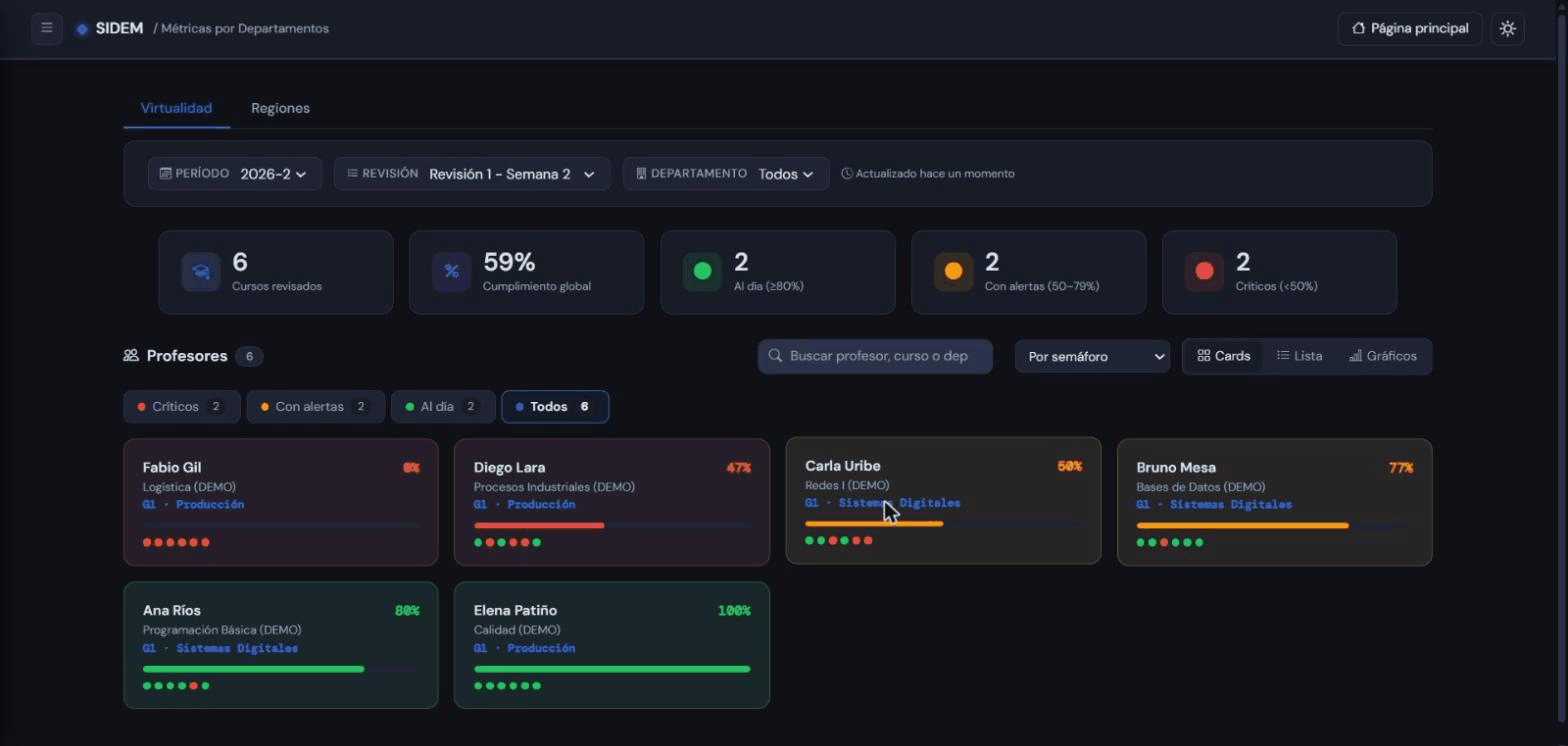
\includegraphics[width=\linewidth,height=5.2cm,keepaspectratio]{figuras/def01-antes.png}\\[2pt]{\small\color{rojo}\textbf{Antes: ve los 6 cursos de la institución.}}\end{minipage}\hfill
\begin{minipage}[t]{0.485\linewidth}\centering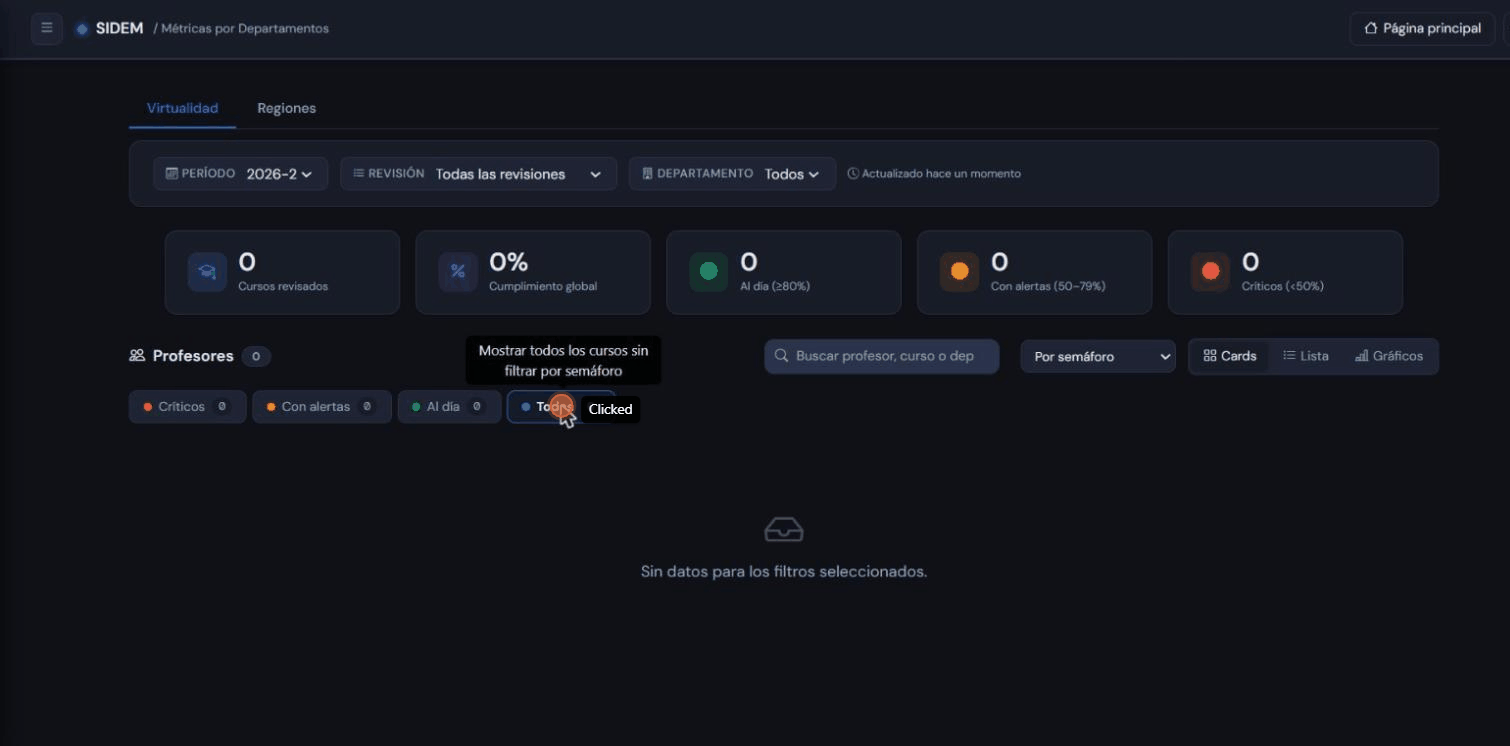
\includegraphics[width=\linewidth,height=5.2cm,keepaspectratio]{figuras/def01-despues.png}\\[2pt]{\small\color{verde}\textbf{Después: 0 cursos y «Sin datos para los filtros seleccionados».}}\end{minipage}
\caption{DEF-01. El líder sin departamento (\code{lider.sindep@sidem.test}) en Métricas, revisión 1.}\end{figure}

\begin{figure}[H]\centering
\begin{minipage}[t]{0.485\linewidth}\centering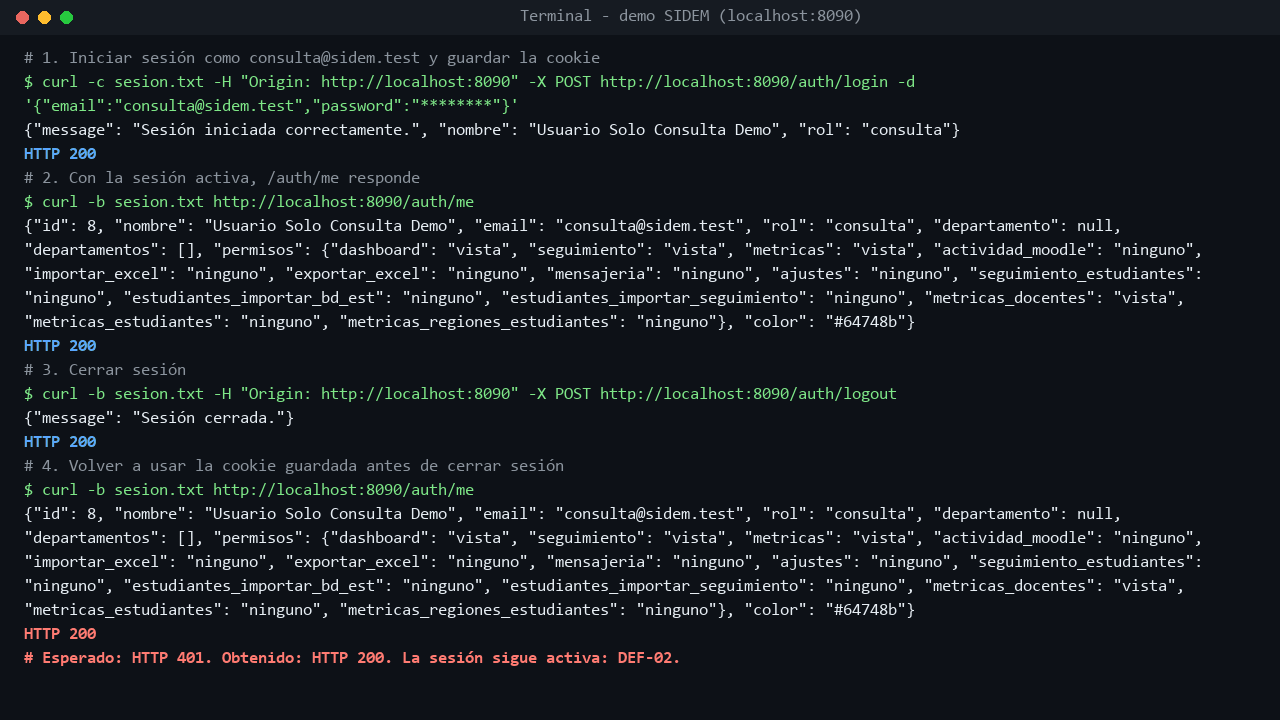
\includegraphics[width=\linewidth,height=5.2cm,keepaspectratio]{figuras/def02-antes.png}\\[2pt]{\small\color{rojo}\textbf{Antes: responde 200 con los datos del usuario.}}\end{minipage}\hfill
\begin{minipage}[t]{0.485\linewidth}\centering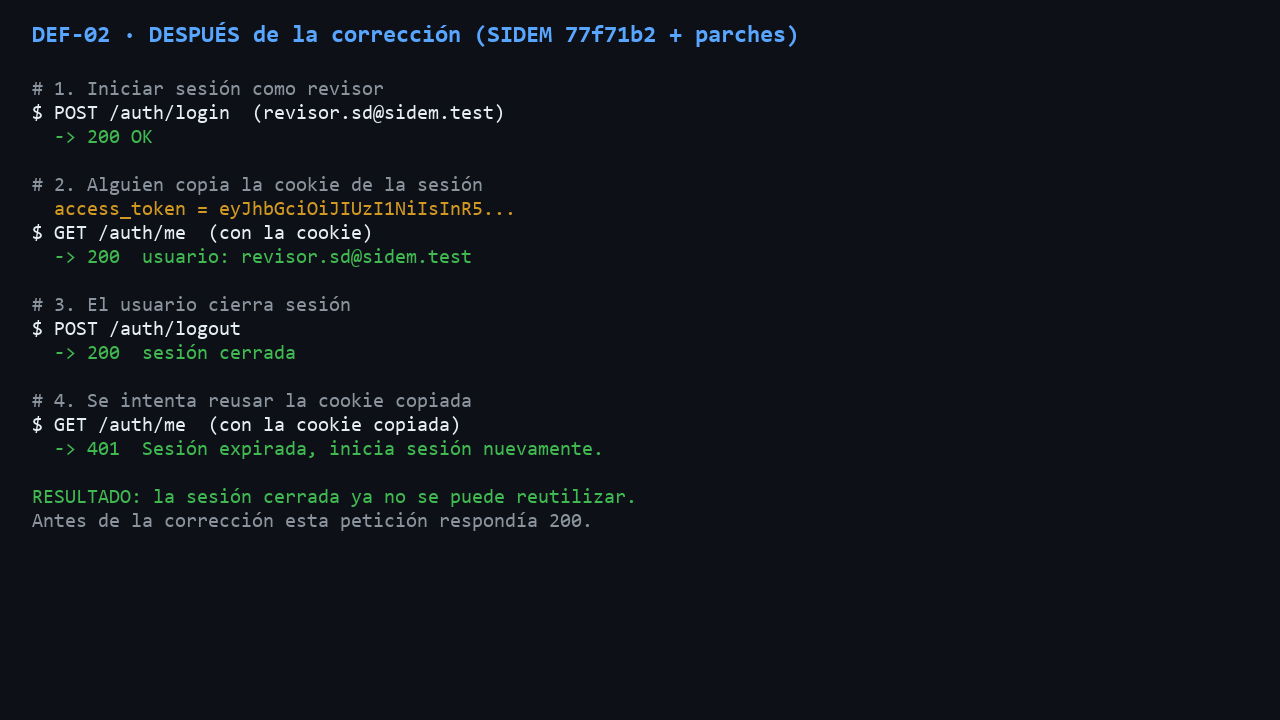
\includegraphics[width=\linewidth,height=5.2cm,keepaspectratio]{figuras/def02-despues.png}\\[2pt]{\small\color{verde}\textbf{Después: responde 401 «Sesión expirada».}}\end{minipage}
\caption{DEF-02. Petición a \code{/auth/me} con la cookie copiada antes de cerrar sesión.}\end{figure}

\begin{figure}[H]\centering
\begin{minipage}[t]{0.485\linewidth}\centering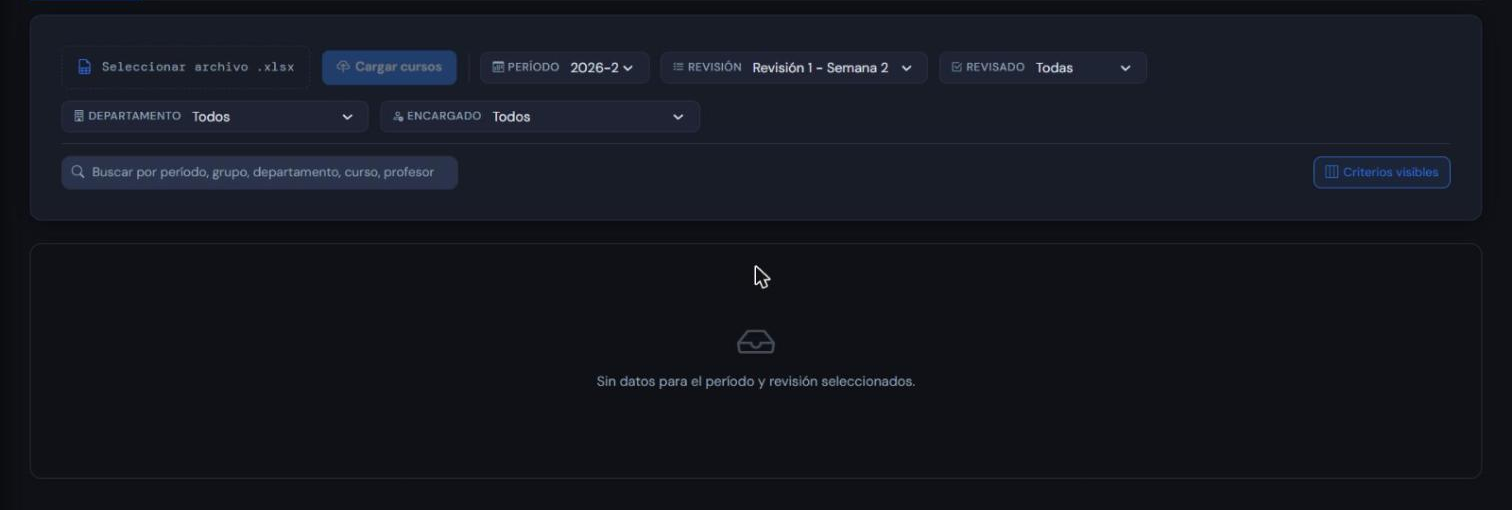
\includegraphics[width=\linewidth,height=5.2cm,keepaspectratio]{figuras/def04-antes.png}\\[2pt]{\small\color{rojo}\textbf{Antes: no ve ningún curso.}}\end{minipage}\hfill
\begin{minipage}[t]{0.485\linewidth}\centering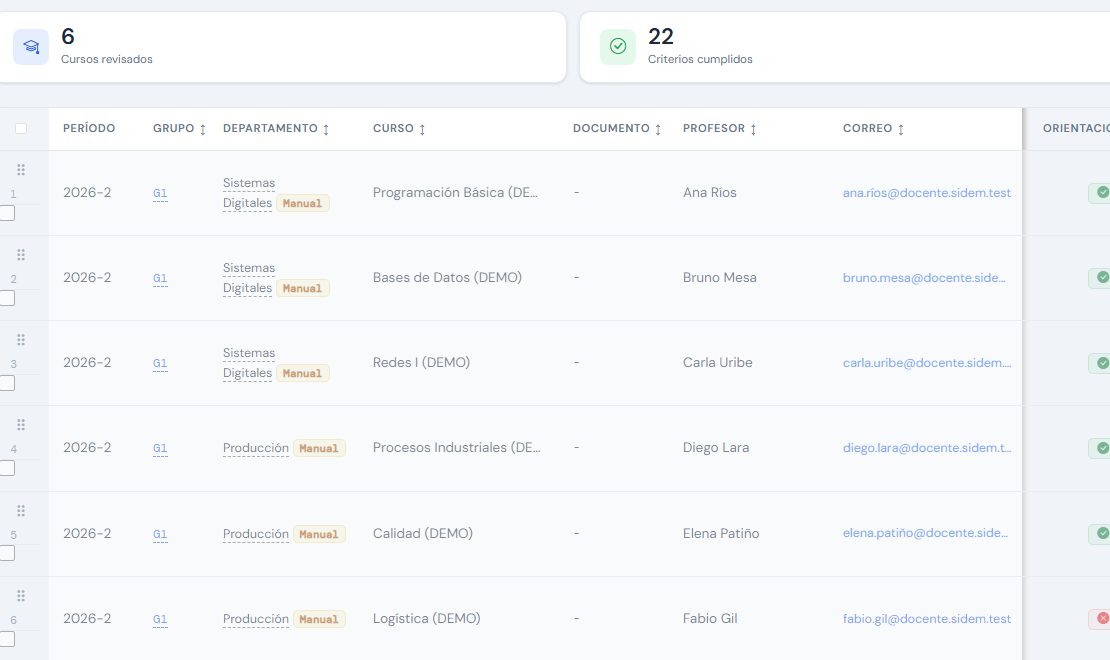
\includegraphics[width=\linewidth,height=5.2cm,keepaspectratio]{figuras/def04-despues.png}\\[2pt]{\small\color{verde}\textbf{Después: con alcance «Todos» ve los 6 cursos.}}\end{minipage}
\caption{DEF-04. El usuario de consulta (\code{consulta@sidem.test}) en Seguimiento, revisión 1.}\end{figure}

\chapter*{Correcciones}\addcontentsline{toc}{chapter}{Correcciones}

Cada archivo \code{.\allowbreak{}patch} corrige un defecto de \code{docs/\allowbreak{}defectos.\allowbreak{}md} sobre la versión de SIDEM que se probó (\code{77f71b2}). Los cambios se ven completos en cada archivo: qué líneas se quitan (\code{-\allowbreak{}}) y cuáles se agregan (\code{+}), junto con la prueba automática que demuestra la corrección.


{\small
\begin{xltabular}{\linewidth}{>{\hsize=0.406\hsize\raggedright\arraybackslash}X>{\hsize=0.406\hsize\raggedright\arraybackslash}X>{\hsize=1.594\hsize\raggedright\arraybackslash}X>{\hsize=1.594\hsize\raggedright\arraybackslash}X}
\hline\rowcolor{cabecera}
\textbf{Parche} & \textbf{Defecto} & \textbf{Qué se cambió} & \textbf{Prueba nueva} \\ \hline
\endhead
\code{0001-\allowbreak{}.\allowbreak{}.\allowbreak{}.\allowbreak{}} & DEF-01 (alta) & En \code{services/\allowbreak{}dashboard\_\allowbreak{}service.\allowbreak{}py}, \code{if dept\_\allowbreak{}lista:\allowbreak{}} pasa a \code{if dept\_\allowbreak{}lista is not None:\allowbreak{}}. La lista vacía significa "ningún departamento", no "todos". & \code{test\_\allowbreak{}lista\_\allowbreak{}vacia\_\allowbreak{}de\_\allowbreak{}departamentos\_\allowbreak{}no\_\allowbreak{}ve\_\allowbreak{}ningun\_\allowbreak{}curso} \\ \hline
\code{0002-\allowbreak{}.\allowbreak{}.\allowbreak{}.\allowbreak{}} & DEF-04 (y DEF-01) & Alcance explícito, como acordó el equipo en los issues \#1 y \#4. El líder de departamento y los roles personalizados se limitan por el departamento asignado: con \textbf{"Todos"} ven todos, con departamentos solo esos y sin ninguno asignado no ven ningún curso. Al crear o editar el usuario el departamento es obligatorio para esos roles, y el formulario de usuarios ofrece la opción "Todos". & \code{test\_\allowbreak{}rol\_\allowbreak{}personalizado\_\allowbreak{}ve\_\allowbreak{}departamentos\_\allowbreak{}segun\_\allowbreak{}asignacion}, \code{test\_\allowbreak{}crear\_\allowbreak{}rol\_\allowbreak{}personalizado\_\allowbreak{}exige\_\allowbreak{}departamento\_\allowbreak{}o\_\allowbreak{}todos}, \code{test\_\allowbreak{}actualizar\_\allowbreak{}a\_\allowbreak{}rol\_\allowbreak{}personalizado\_\allowbreak{}sin\_\allowbreak{}departamento\_\allowbreak{}se\_\allowbreak{}rechaza} \\ \hline
\code{0003-\allowbreak{}.\allowbreak{}.\allowbreak{}.\allowbreak{}} & DEF-02 & Contador de sesión \code{token\_\allowbreak{}version} en \code{usuarios}, como propuso Sebastián en el issue \#2. Va en cada token y \code{logout()} lo incrementa, así el token copiado deja de servir aunque el login y el logout pasen en el mismo segundo (el caso de TC-06). Cierra todas las sesiones del usuario. \code{db.\allowbreak{}sql} agrega la columna. & \code{TestLogout} en \code{test\_\allowbreak{}auth.\allowbreak{}py}, incluido \code{test\_\allowbreak{}token\_\allowbreak{}copiado\_\allowbreak{}no\_\allowbreak{}sirve\_\allowbreak{}aunque\_\allowbreak{}logout\_\allowbreak{}sea\_\allowbreak{}en\_\allowbreak{}el\_\allowbreak{}mismo\_\allowbreak{}segundo} \\ \hline
\code{0004-\allowbreak{}.\allowbreak{}.\allowbreak{}.\allowbreak{}} & DEF-03 & La fecha de \code{log\_\allowbreak{}actividad} la pone la aplicación en UTC, no la base. \code{db.\allowbreak{}sql} sin \code{AT TIME ZONE}. & \code{test\_\allowbreak{}log\_\allowbreak{}service.\allowbreak{}py} \\ \hline
\code{0005-\allowbreak{}.\allowbreak{}.\allowbreak{}.\allowbreak{}} & DEF-05 & En \code{db.\allowbreak{}sql}, el backfill de \code{estado\_\allowbreak{}seguimiento} solo corre si la columna vieja existe. & Se instaló \code{db.\allowbreak{}sql} en un PostgreSQL vacío: antes fallaba en la línea 597, ahora termina sin errores. \\ \hline
\end{xltabular}}


Con los 5 parches aplicados pasan las 650 pruebas automáticas de SIDEM.


En la demo, \code{seed\_\allowbreak{}demo.\allowbreak{}py} le asigna "Todos" a \code{consulta@sidem.\allowbreak{}test}, para que TC-02 pruebe un rol personalizado que debe ver el seguimiento completo. \code{lider.\allowbreak{}sindep@sidem.\allowbreak{}test} sigue sin departamento para probar que no ve nada. El seed solo crea los usuarios que faltan, así que hay que partir de una base nueva.


\section*{Cómo se usan}\addcontentsline{toc}{section}{Cómo se usan}

Los aplica el líder al reconstruir las imágenes de la demo (ver \code{demo/\allowbreak{}README.\allowbreak{}md}):


\begin{lstlisting}
git am demo/correcciones/*.patch
\end{lstlisting}

\chapter*{Retest}\addcontentsline{toc}{chapter}{Retest}

Guía para repetir las pruebas sobre SIDEM con las correcciones de DEF-01 a DEF-05. Lo ejecuta \textbf{Sebastián}; con el resultado se actualiza el informe de cierre.


\begin{nota}
\textbf{Hecho el 16/11/2026 por Sebastián:} 19 de 19 pruebas pasan y los 5 defectos quedan cerrados. Detalle en \code{defectos.\allowbreak{}md} y en \code{evidencias/\allowbreak{}pytest/\allowbreak{}ejecucion\_\allowbreak{}2026-\allowbreak{}11-\allowbreak{}16\_\allowbreak{}retest\_\allowbreak{}Sebastian.\allowbreak{}txt}. Los issues \#1 a \#5 quedaron cerrados con el resultado y el informe de cierre está en su versión final (1.0).

\end{nota}

\section*{Qué cambió}\addcontentsline{toc}{section}{Qué cambió}

\begin{itemize}
\item \textbf{Versión probada:} commit \code{77f71b2} más los parches \code{0001} a \code{0005} de \code{demo/\allowbreak{}correcciones/\allowbreak{}}. Las imágenes de Docker se llaman \code{sidem-\allowbreak{}demo-\allowbreak{}app:\allowbreak{}77f71b2-\allowbreak{}correcciones} y \code{sidem-\allowbreak{}demo-\allowbreak{}db:\allowbreak{}77f71b2-\allowbreak{}correcciones}.
\item \textbf{Base de datos en UTC.} En la primera ronda estaba en \code{America/\allowbreak{}Bogota} para que TC-09 pasara. Ahora queda en UTC para comprobar que DEF-03 está corregido.
\item \textbf{Usuario \code{consulta@sidem.\allowbreak{}test}} con alcance "Todos" (DEF-04). \code{lider.\allowbreak{}sindep@sidem.\allowbreak{}test} sigue sin departamento (DEF-01).
\end{itemize}

{\small
\begin{xltabular}{\linewidth}{>{\hsize=0.426\hsize\raggedright\arraybackslash}X>{\hsize=1.664\hsize\raggedright\arraybackslash}X>{\hsize=0.910\hsize\raggedright\arraybackslash}X}
\hline\rowcolor{cabecera}
\textbf{Defecto} & \textbf{Caso que lo comprueba} & \textbf{Resultado esperado en el retest} \\ \hline
\endhead
DEF-01 & TC-02 (\code{test\_\allowbreak{}lider\_\allowbreak{}sin\_\allowbreak{}departamento\_\allowbreak{}no\_\allowbreak{}ve\_\allowbreak{}metricas}) & El líder sin departamento ve 0 cursos. \\ \hline
DEF-02 & TC-06 (\code{test\_\allowbreak{}sesion\_\allowbreak{}cerrada\_\allowbreak{}no\_\allowbreak{}se\_\allowbreak{}reutiliza}) & La cookie copiada antes de cerrar sesión da 401. \\ \hline
DEF-03 & TC-09 (\code{test\_\allowbreak{}bloqueo\_\allowbreak{}y\_\allowbreak{}desbloqueo}) & El bloqueo funciona con la base en UTC. \\ \hline
DEF-04 & TC-02 (\code{test\_\allowbreak{}consulta\_\allowbreak{}puede\_\allowbreak{}ver\_\allowbreak{}el\_\allowbreak{}seguimiento}) & El usuario de consulta ve los 6 cursos. \\ \hline
DEF-05 & Log de la base al crearla & \code{db.\allowbreak{}sql} termina sin líneas \code{ERROR}. \\ \hline
\end{xltabular}}


\section*{Pasos}\addcontentsline{toc}{section}{Pasos}

\begin{enumerate}
\item \textbf{Descargar las imágenes.} Baja \code{sidem-\allowbreak{}demo-\allowbreak{}imagenes-\allowbreak{}77f71b2-\allowbreak{}correcciones.\allowbreak{}tar.\allowbreak{}gz} (unos 264 MB) de la \href{https://drive.google.com/drive/folders/1i7nXTlf7k8DhToZPXx2Hm70bDSp-vvhp?usp=drive_link}{carpeta de Drive del equipo} (ya está subido) y cárgalo:
\end{enumerate}

\begin{lstlisting}
docker load -i sidem-demo-imagenes-77f71b2-correcciones.tar.gz
\end{lstlisting}

Debe terminar con \code{Loaded image:\allowbreak{} sidem-\allowbreak{}demo-\allowbreak{}app:\allowbreak{}77f71b2-\allowbreak{}correcciones} y \code{Loaded image:\allowbreak{} sidem-\allowbreak{}demo-\allowbreak{}db:\allowbreak{}77f71b2-\allowbreak{}correcciones}.


\begin{enumerate}[start=2]
\item \textbf{Actualizar el repositorio y levantar la demo desde cero} (desde \code{demo/\allowbreak{}}). El \code{down -\allowbreak{}v} borra la base de la demo anterior; es necesario porque el seed solo crea los usuarios que faltan.
\end{enumerate}

\begin{lstlisting}
git pull
docker compose down -v
docker compose up -d
\end{lstlisting}

\begin{enumerate}[start=3]
\item \textbf{Comprobar DEF-05.} Debe responder \code{0}:
\end{enumerate}

\begin{lstlisting}
docker logs sidem-demo-db 2>&1 | Select-String "ERROR:" | Measure-Object | Select-Object -ExpandProperty Count
\end{lstlisting}

Si quieres revisar la zona horaria: \code{docker exec sidem-\allowbreak{}demo-\allowbreak{}db psql -\allowbreak{}U sidem -\allowbreak{}d seguimiento\_\allowbreak{}docentes -\allowbreak{}tAc "show timezone"} debe decir \code{UTC}.


\begin{enumerate}[start=4]
\item \textbf{Correr las pruebas automáticas} (desde \code{pruebas-\allowbreak{}automaticas/\allowbreak{}}, unos 7 minutos):
\end{enumerate}

\begin{lstlisting}
python -m pytest -rA --junitxml=..\evidencias\pytest\ejecucion_AAAA-MM-DD_retest_Sebastian.xml | Tee-Object ..\evidencias\pytest\ejecucion_AAAA-MM-DD_retest_Sebastian.txt
\end{lstlisting}

Resultado esperado: \textbf{19 pasan, 0 fallan}. En la primera ronda fallaban 3 (TC-02 ×2 por DEF-01 y DEF-04, y TC-06 por DEF-02).


\begin{enumerate}[start=5]
\item \textbf{Repetir a mano lo que quieras mostrar} (opcional), con la hoja de \code{ejecucion-\allowbreak{}manual.\allowbreak{}md}. Por ejemplo, \code{lider.\allowbreak{}sindep@sidem.\allowbreak{}test} en Métricas debe ver "Sin datos".
\end{enumerate}

\section*{Qué registrar después}\addcontentsline{toc}{section}{Qué registrar después}

{\small
\begin{xltabular}{\linewidth}{>{\hsize=0.432\hsize\raggedright\arraybackslash}X>{\hsize=1.531\hsize\raggedright\arraybackslash}X>{\hsize=1.037\hsize\raggedright\arraybackslash}X}
\hline\rowcolor{cabecera}
\textbf{Quién} & \textbf{Dónde} & \textbf{Qué} \\ \hline
\endhead
Sebastián & \code{evidencias/\allowbreak{}pytest/\allowbreak{}} & Los archivos \code{.\allowbreak{}txt} y \code{.\allowbreak{}xml} del paso 4. \\ \hline
Sebastián & \code{defectos.\allowbreak{}md} & Estado de cada defecto: "Cerrado (retest DD/11)" si pasa, o "Reabierto" con lo que se vio. \\ \hline
Sebastián & Issues \#1 a \#5 en GitHub & Comentario con el resultado; cerrar el issue si pasa. \\ \hline
Sebastián & \code{avances.\allowbreak{}md} & Una fila con la corrida. \\ \hline
Marcos y Nicolás & \code{informe-\allowbreak{}de-\allowbreak{}cierre.\allowbreak{}md} & Sección de retest, estado final de los defectos y criterios de finalización. \\ \hline
\end{xltabular}}


\section*{Verificación previa}\addcontentsline{toc}{section}{Verificación previa}

El 16/11/2026 Marcos armó las imágenes y las probó en una base nueva: \code{db.\allowbreak{}sql} cargó sin errores, la base quedó en UTC y las 19 pruebas pasaron. Esa corrida no reemplaza el retest; sirve para saber que la imagen está bien antes de entregarla.


\part*{Parte IV. Informe de cierre}


\chapter*{Informe de cierre}\addcontentsline{toc}{chapter}{Informe de cierre}

\begin{nota}
Basado en la norma ISO/IEC/IEEE 29119-3 (\emph{Test Completion Report}). Es el documento final de la entrega (confirmado con el docente el 16/11, pregunta 8 de \code{preguntas-\allowbreak{}para-\allowbreak{}el-\allowbreak{}profe.\allowbreak{}md}). \textbf{Estado:} versión 1.0, final. Incluye la primera ronda de ejecución (08 y 12/11/2026) y el retest de las correcciones (16/11/2026).

\end{nota}

\section*{1. Información del documento}\addcontentsline{toc}{section}{1. Información del documento}

{\small
\begin{xltabular}{\linewidth}{>{\hsize=0.684\hsize\raggedright\arraybackslash}X>{\hsize=1.316\hsize\raggedright\arraybackslash}X}
\hline\rowcolor{cabecera}
\textbf{Campo} & \textbf{Valor} \\ \hline
\endhead
Identificador & \code{SIDEM-\allowbreak{}IC-\allowbreak{}2026-\allowbreak{}01} \\ \hline
Versión & 1.0 (final) \\ \hline
Fecha & 17/11/2026 \\ \hline
Autores & Marcos Duque Jaramillo, Sebastián Díaz Jiménez, Nicolás Cataño Durango, Julián Ramírez Molina \\ \hline
Plan al que responde & \code{SIDEM-\allowbreak{}PP-\allowbreak{}2026-\allowbreak{}01}, versión 1.0 (\code{docs/\allowbreak{}plan-\allowbreak{}de-\allowbreak{}pruebas.\allowbreak{}md}) \\ \hline
Aprobación & Roberto José Calderón Bermejo, docente del curso \\ \hline
\end{xltabular}}


\textbf{Historial del informe:}


{\small
\begin{xltabular}{\linewidth}{>{\hsize=0.435\hsize\raggedright\arraybackslash}X>{\hsize=0.438\hsize\raggedright\arraybackslash}X>{\hsize=0.666\hsize\raggedright\arraybackslash}X>{\hsize=2.461\hsize\raggedright\arraybackslash}X}
\hline\rowcolor{cabecera}
\textbf{Versión} & \textbf{Fecha} & \textbf{Quién} & \textbf{Cambio} \\ \hline
\endhead
0.1 & 12/11/2026 & Julián Ramírez Molina & Primera versión con la ejecución registrada hasta el 12/11. \\ \hline
1.0 & 17/11/2026 & Marcos Duque Jaramillo y Nicolás Cataño Durango & Versión final: ejecución manual completa, retest del 16/11, defectos cerrados, criterios de finalización y lecciones aprendidas. Marcos, como encargado de organizar la exposición, consolidó con Nicolás el cierre del informe y las láminas de cierre. \\ \hline
\end{xltabular}}


\textbf{Fuentes usadas:} \code{docs/\allowbreak{}ejecucion-\allowbreak{}manual.\allowbreak{}md}, \code{docs/\allowbreak{}defectos.\allowbreak{}md}, \code{docs/\allowbreak{}retest.\allowbreak{}md}, \code{docs/\allowbreak{}avances.\allowbreak{}md}, \code{evidencias/\allowbreak{}README.\allowbreak{}md} y las salidas de pytest de \code{evidencias/\allowbreak{}pytest/\allowbreak{}} (08/11, 12/11 y retest del 16/11).


\section*{2. Resumen}\addcontentsline{toc}{section}{2. Resumen}

Se probó SIDEM (FastAPI + PostgreSQL), versión commit \code{77f71b2}, en una copia de demostración con Docker y datos ficticios (entorno AMB-01, datos DAT-01). No se usó Moodle ni la base de producción.


\textbf{Primera ronda (08 y 12/11/2026).} Las pruebas automáticas con pytest se corrieron dos veces con la demo recién reiniciada, en computadores distintos, con el mismo resultado: 19 pruebas, 16 pasan y 3 fallan. El 12/11 el equipo ejecutó a mano los 8 casos con parte manual (TC-01 a TC-08), con capturas en \code{evidencias/\allowbreak{}}. Se registraron 5 defectos (DEF-01 a DEF-05): 1 alto, 2 medios y 2 bajos.


\textbf{Correcciones y retest (16/11/2026).} Cada defecto se corrigió con un parche sobre \code{77f71b2} (\code{demo/\allowbreak{}correcciones/\allowbreak{}}, parches \code{0001} a \code{0005}), cada uno con su prueba automática. En el retest, con las imágenes \code{77f71b2-\allowbreak{}correcciones} y la base en UTC, pasan las 19 pruebas y \code{db.\allowbreak{}sql} se instala sin errores. Los 5 defectos quedan cerrados.


\textbf{Resultado final:} los 9 casos planeados (TC-01 a TC-09) están ejecutados y pasan, no queda ningún defecto abierto y se cumplen todos los criterios de finalización del plan (sección 7).


\section*{3. Lo que se ejecutó}\addcontentsline{toc}{section}{3. Lo que se ejecutó}

\subsection*{3.1 Resultado por caso}\addcontentsline{toc}{subsection}{3.1 Resultado por caso}

"Auto" es pytest contra la demo. "Manual" es la ejecución en el navegador con la hoja de \code{ejecucion-\allowbreak{}manual.\allowbreak{}md} (12/11/2026). "Primera ronda" es el resultado con \code{77f71b2} sin cambios y "Retest" con las correcciones.


{\scriptsize
\begin{xltabular}{\linewidth}{>{\hsize=0.528\hsize\raggedright\arraybackslash}X>{\hsize=0.951\hsize\raggedright\arraybackslash}X>{\hsize=1.057\hsize\raggedright\arraybackslash}X>{\hsize=1.585\hsize\raggedright\arraybackslash}X>{\hsize=1.275\hsize\raggedright\arraybackslash}X>{\hsize=0.740\hsize\raggedright\arraybackslash}X>{\hsize=1.123\hsize\raggedright\arraybackslash}X>{\hsize=0.740\hsize\raggedright\arraybackslash}X}
\hline\rowcolor{cabecera}
\textbf{Caso} & \textbf{Prioridad} & \textbf{Tipo planeado} & \textbf{Auto (primera ronda)} & \textbf{Manual} & \textbf{Primera ronda} & \textbf{Retest (16/11)} & \textbf{Defecto} \\ \hline
\endhead
TC-01 & P1 & Manual + automática & 3 de 3 pasan & 4 de 4 pasos pasan & Pasa & Pasa (3 de 3) & - \\ \hline
TC-02 & P1 & Manual + automática & 2 de 4 pasan, 2 fallan & Pasos 1 y 3 fallan; paso 2 cubierto en lo automático & Falla & Pasa (4 de 4) & DEF-01, DEF-04 \\ \hline
TC-03 & P1 & Manual + automática & 7 de 7 pasan & 7 de 7 pasos pasan & Pasa & Pasa (7 de 7) & - \\ \hline
TC-07 & P1 & Manual + automática & 1 de 1 pasa & 4 de 4 pasos pasan & Pasa & Pasa (1 de 1) & - \\ \hline
TC-04 & P2 & Manual & No aplica & 4 de 4 pasos pasan & Pasa & No aplica (sin defecto) & - \\ \hline
TC-08 & P2 & Manual & No aplica & 3 de 3 pasos pasan & Pasa & No aplica (sin defecto) & - \\ \hline
TC-05 & P2 & Manual + automática & 2 de 2 pasan & 4 de 4 pasos pasan & Pasa & Pasa (2 de 2) & - \\ \hline
TC-09 & P2 & Automática & 1 de 1 pasa (base en \code{America/\allowbreak{}Bogota}) & No aplica & Pasa & Pasa con la base en UTC (1 de 1) & DEF-03 \\ \hline
TC-06 & P3 & Manual & 0 de 1 pasan (complemento automático) & 4 de 4 pasos pasan & Falla & Pasa (1 de 1) & DEF-02 \\ \hline
\end{xltabular}}


Quién ejecutó:


{\small
\begin{xltabular}{\linewidth}{>{\hsize=0.427\hsize\raggedright\arraybackslash}X>{\hsize=0.427\hsize\raggedright\arraybackslash}X>{\hsize=2.146\hsize\raggedright\arraybackslash}X}
\hline\rowcolor{cabecera}
\textbf{Caso} & \textbf{Responsable} & \textbf{Ejecución registrada} \\ \hline
\endhead
TC-01, TC-02 & Marcos & Manual el 12/11 (\code{evidencias/\allowbreak{}TC-\allowbreak{}01\_\allowbreak{}2026-\allowbreak{}11-\allowbreak{}12\_\allowbreak{}Marcos\_\allowbreak{}*}, \code{TC-\allowbreak{}02\_\allowbreak{}2026-\allowbreak{}11-\allowbreak{}12\_\allowbreak{}Marcos\_\allowbreak{}*}). \\ \hline
TC-07, TC-04 & Sebastián & Manual el 12/11 (\code{evidencias/\allowbreak{}TC-\allowbreak{}07\_\allowbreak{}2026-\allowbreak{}11-\allowbreak{}12\_\allowbreak{}Sebastian*}, \code{TC-\allowbreak{}04\_\allowbreak{}2026-\allowbreak{}11-\allowbreak{}12\_\allowbreak{}Sebastian*}). Corrida de pytest del 12/11 y retest del 16/11. \\ \hline
TC-03, TC-08 & Nicolás & Manual el 12/11 (\code{evidencias/\allowbreak{}TC-\allowbreak{}03\_\allowbreak{}2026-\allowbreak{}11-\allowbreak{}12\_\allowbreak{}Nicolas.\allowbreak{}png}, \code{TC-\allowbreak{}08\_\allowbreak{}2026-\allowbreak{}11-\allowbreak{}12\_\allowbreak{}Nicolas\_\allowbreak{}*}). \\ \hline
TC-05, TC-06, TC-09 & Julián & Manual de TC-05 y TC-06 el 12/11 (\code{evidencias/\allowbreak{}TC-\allowbreak{}05\_\allowbreak{}2026-\allowbreak{}11-\allowbreak{}12\_\allowbreak{}Julian\_\allowbreak{}*}, \code{TC-\allowbreak{}06\_\allowbreak{}2026-\allowbreak{}11-\allowbreak{}12\_\allowbreak{}Julian\_\allowbreak{}*}) y revisión de la salida de pytest de TC-09. \\ \hline
\end{xltabular}}


\subsection*{3.2 Notas sobre los casos}\addcontentsline{toc}{subsection}{3.2 Notas sobre los casos}

\begin{itemize}
\item \textbf{TC-01.} El líder de Sistemas Digitales solo ve su departamento, no puede forzar el de Producción y no puede modificar el seguimiento. Los criterios de Logística siguen sin cambios al revisarlos como administrador.
\item \textbf{TC-02.} En la primera ronda, el usuario de consulta veía 0 cursos en vez de 6 (DEF-04) y el líder sin departamento veía los 6 cursos en vez de 0 (DEF-01). El paso 2 (intentar guardar) no se pudo hacer a mano porque el usuario de consulta no veía cursos; lo cubre \code{test\_\allowbreak{}consulta\_\allowbreak{}no\_\allowbreak{}puede\_\allowbreak{}guardar}, que pasa en las tres corridas. En el retest, consulta ve los 6 cursos sin poder guardar y el líder sin departamento ve 0 cursos y "Sin datos".
\item \textbf{TC-03 y TC-08.} Los 6 cursos muestran 80, 77, 50, 47, 100 y 0 \% con el color esperado (verde, amarillo, amarillo, rojo, verde y rojo), y el panel da 6 cursos: 2 al día, 2 con alertas y 2 críticos. En TC-08, Sistemas Digitales da 3 cursos (1 al día, 2 con alertas, 0 críticos) y Producción 3 cursos (1 al día, 0 con alertas, 2 críticos). TC-08 se ejecutó sin \code{docker compose down -\allowbreak{}v} previo; los datos de la revisión 1 coincidían con \code{demo/\allowbreak{}seed\_\allowbreak{}demo.\allowbreak{}py}.
\item \textbf{TC-04 y TC-07.} Lo guardado en la revisión 2 se conserva al recargar y al volver a entrar, y queda en el curso y la revisión correctos sin tocar la revisión 1.
\item \textbf{TC-05.} Los Excel de Sistemas Digitales y de Producción traen los mismos cursos y los mismos SI/NO de la revisión 1 que la pantalla de Seguimiento.
\item \textbf{TC-06.} En el navegador, cerrar sesión lleva al login, "Atrás" deja el login y recargar sigue en el login. En la primera ronda, la prueba automática mostró que la cookie copiada antes del cierre seguía sirviendo (200 en lugar de 401, DEF-02). En el retest da 401.
\item \textbf{TC-09.} En la primera ronda el bloqueo solo funcionó con la base en \code{America/\allowbreak{}Bogota} (DEF-03). En el retest, con la base en UTC, los 5 intentos fallidos dan 401, el 6.º con la clave correcta da 429 y pasados los 300 s vuelve a entrar.
\end{itemize}

\subsection*{3.3 Trazabilidad}\addcontentsline{toc}{subsection}{3.3 Trazabilidad}

{\footnotesize
\begin{xltabular}{\linewidth}{>{\hsize=0.445\hsize\raggedright\arraybackslash}X>{\hsize=0.627\hsize\raggedright\arraybackslash}X>{\hsize=0.445\hsize\raggedright\arraybackslash}X>{\hsize=2.856\hsize\raggedright\arraybackslash}X>{\hsize=0.627\hsize\raggedright\arraybackslash}X}
\hline\rowcolor{cabecera}
\textbf{Riesgo} & \textbf{Condición} & \textbf{Caso} & \textbf{Evidencia} & \textbf{Defecto} \\ \hline
\endhead
R01 & CP-01, CP-02 & TC-01, TC-02 & \code{evidencias/\allowbreak{}TC-\allowbreak{}01\_\allowbreak{}*}, \code{evidencias/\allowbreak{}TC-\allowbreak{}02\_\allowbreak{}*}, \code{evidencias/\allowbreak{}pytest/\allowbreak{}} & DEF-04 (cerrado) \\ \hline
R02 & CP-02 & TC-02 & \code{evidencias/\allowbreak{}TC-\allowbreak{}02\_\allowbreak{}*}, \code{evidencias/\allowbreak{}pytest/\allowbreak{}} & DEF-01 (cerrado) \\ \hline
R03 & CP-03 & TC-07 & \code{evidencias/\allowbreak{}TC-\allowbreak{}07\_\allowbreak{}*}, \code{evidencias/\allowbreak{}pytest/\allowbreak{}} & - \\ \hline
R04 & CP-04 & TC-03 & \code{evidencias/\allowbreak{}TC-\allowbreak{}03\_\allowbreak{}2026-\allowbreak{}11-\allowbreak{}12\_\allowbreak{}Nicolas.\allowbreak{}png}, \code{evidencias/\allowbreak{}pytest/\allowbreak{}} & - \\ \hline
R05 & CP-05 & TC-04 & \code{evidencias/\allowbreak{}TC-\allowbreak{}04\_\allowbreak{}*} & - \\ \hline
R06 & CP-06 & TC-08 & \code{evidencias/\allowbreak{}TC-\allowbreak{}08\_\allowbreak{}2026-\allowbreak{}11-\allowbreak{}12\_\allowbreak{}Nicolas\_\allowbreak{}*.\allowbreak{}png} & - \\ \hline
R07 & CP-07 & TC-05 & \code{evidencias/\allowbreak{}TC-\allowbreak{}05\_\allowbreak{}2026-\allowbreak{}11-\allowbreak{}12\_\allowbreak{}Julian\_\allowbreak{}*}, \code{evidencias/\allowbreak{}pytest/\allowbreak{}} & - \\ \hline
R08 & CP-08 & TC-09 & \code{evidencias/\allowbreak{}pytest/\allowbreak{}} & DEF-03 (cerrado) \\ \hline
R09 & CP-09 & TC-06 & \code{evidencias/\allowbreak{}TC-\allowbreak{}06\_\allowbreak{}2026-\allowbreak{}11-\allowbreak{}12\_\allowbreak{}Julian\_\allowbreak{}*}, \code{evidencias/\allowbreak{}pytest/\allowbreak{}} & DEF-02 (cerrado) \\ \hline
\end{xltabular}}


\section*{4. Métricas}\addcontentsline{toc}{section}{4. Métricas}

\subsection*{4.1 Casos}\addcontentsline{toc}{subsection}{4.1 Casos}

{\small
\begin{xltabular}{\linewidth}{>{\hsize=1.294\hsize\raggedright\arraybackslash}X>{\hsize=0.853\hsize\raggedright\arraybackslash}X>{\hsize=0.853\hsize\raggedright\arraybackslash}X}
\hline\rowcolor{cabecera}
\textbf{Métrica} & \textbf{Primera ronda} & \textbf{Después del retest} \\ \hline
\endhead
Casos planeados (TC-01 a TC-09) & 9 & 9 \\ \hline
Casos ejecutados & 9 & 9 \\ \hline
Casos que pasan & 7 & 9 \\ \hline
Casos que fallan & 2 (TC-02 y TC-06) & 0 \\ \hline
\end{xltabular}}


Los casos extra TC-10 a TC-17 quedaron identificados en el plan (v0.4) y no se ejecutan en este ciclo, como se acordó con el docente.


\subsection*{4.2 Pruebas automáticas (pytest)}\addcontentsline{toc}{subsection}{4.2 Pruebas automáticas (pytest)}

{\footnotesize
\begin{xltabular}{\linewidth}{>{\hsize=1.486\hsize\raggedright\arraybackslash}X>{\hsize=0.946\hsize\raggedright\arraybackslash}X>{\hsize=0.676\hsize\raggedright\arraybackslash}X>{\hsize=0.811\hsize\raggedright\arraybackslash}X>{\hsize=1.081\hsize\raggedright\arraybackslash}X}
\hline\rowcolor{cabecera}
\textbf{Corrida} & \textbf{Pruebas} & \textbf{Pasan} & \textbf{Fallan} & \textbf{Duración} \\ \hline
\endhead
08/11/2026 & 19 & 16 & 3 & 365,77 s \\ \hline
12/11/2026 (Sebastián) & 19 & 16 & 3 & 367,94 s \\ \hline
16/11/2026, retest (Sebastián) & 19 & 19 & 0 & 368,28 s \\ \hline
\end{xltabular}}


En la primera ronda fallaban \code{test\_\allowbreak{}consulta\_\allowbreak{}puede\_\allowbreak{}ver\_\allowbreak{}el\_\allowbreak{}seguimiento} (DEF-04), \code{test\_\allowbreak{}lider\_\allowbreak{}sin\_\allowbreak{}departamento\_\allowbreak{}no\_\allowbreak{}ve\_\allowbreak{}metricas} (DEF-01) y \code{test\_\allowbreak{}sesion\_\allowbreak{}cerrada\_\allowbreak{}no\_\allowbreak{}se\_\allowbreak{}reutiliza} (DEF-02). En el retest pasan las tres.


\subsection*{4.3 Pasos manuales}\addcontentsline{toc}{subsection}{4.3 Pasos manuales}

{\footnotesize
\begin{xltabular}{\linewidth}{>{\hsize=0.781\hsize\raggedright\arraybackslash}X>{\hsize=0.781\hsize\raggedright\arraybackslash}X>{\hsize=0.781\hsize\raggedright\arraybackslash}X>{\hsize=1.250\hsize\raggedright\arraybackslash}X>{\hsize=1.406\hsize\raggedright\arraybackslash}X}
\hline\rowcolor{cabecera}
\textbf{Caso} & \textbf{Pasos} & \textbf{Pasan} & \textbf{Fallan} & \textbf{Sin ejecutar a mano} \\ \hline
\endhead
TC-01 & 4 & 4 & 0 & 0 \\ \hline
TC-02 & 3 & 0 & 2 (DEF-04, DEF-01) & 1 (cubierto por pytest) \\ \hline
TC-03 & 7 & 7 & 0 & 0 \\ \hline
TC-04 & 4 & 4 & 0 & 0 \\ \hline
TC-05 & 4 & 4 & 0 & 0 \\ \hline
TC-06 & 4 & 4 & 0 & 0 \\ \hline
TC-07 & 4 & 4 & 0 & 0 \\ \hline
TC-08 & 3 & 3 & 0 & 0 \\ \hline
\end{xltabular}}


Los dos pasos que fallaron en TC-02 se revisaron otra vez en el navegador en el retest (\code{evidencias/\allowbreak{}TC-\allowbreak{}02\_\allowbreak{}2026-\allowbreak{}11-\allowbreak{}16\_\allowbreak{}retest\_\allowbreak{}Sebastian\_\allowbreak{}*}) y dan lo esperado.


\subsection*{4.4 Defectos por severidad}\addcontentsline{toc}{subsection}{4.4 Defectos por severidad}

{\small
\begin{xltabular}{\linewidth}{>{\hsize=1.000\hsize\raggedright\arraybackslash}X>{\hsize=1.222\hsize\raggedright\arraybackslash}X>{\hsize=0.889\hsize\raggedright\arraybackslash}X>{\hsize=0.889\hsize\raggedright\arraybackslash}X}
\hline\rowcolor{cabecera}
\textbf{Severidad} & \textbf{Encontrados} & \textbf{Cerrados} & \textbf{Abiertos} \\ \hline
\endhead
Crítica & 0 & 0 & 0 \\ \hline
Alta & 1 (DEF-01) & 1 & 0 \\ \hline
Media & 2 (DEF-02, DEF-03) & 2 & 0 \\ \hline
Baja & 2 (DEF-04, DEF-05) & 2 & 0 \\ \hline
\textbf{Total} & \textbf{5} & \textbf{5} & \textbf{0} \\ \hline
\end{xltabular}}


\section*{5. Defectos}\addcontentsline{toc}{section}{5. Defectos}

Detalle en \code{docs/\allowbreak{}defectos.\allowbreak{}md}. Versión de SIDEM: commit \code{77f71b2}; correcciones en \code{demo/\allowbreak{}correcciones/\allowbreak{}}.


{\scriptsize
\begin{xltabular}{\linewidth}{>{\hsize=0.428\hsize\raggedright\arraybackslash}X>{\hsize=0.428\hsize\raggedright\arraybackslash}X>{\hsize=0.428\hsize\raggedright\arraybackslash}X>{\hsize=0.497\hsize\raggedright\arraybackslash}X>{\hsize=2.162\hsize\raggedright\arraybackslash}X>{\hsize=2.391\hsize\raggedright\arraybackslash}X>{\hsize=0.667\hsize\raggedright\arraybackslash}X}
\hline\rowcolor{cabecera}
\textbf{ID} & \textbf{Caso} & \textbf{Riesgo} & \textbf{Severidad} & \textbf{Qué pasaba} & \textbf{Corrección} & \textbf{Estado} \\ \hline
\endhead
DEF-01 & TC-02 & R02 & Alta & El líder de departamento sin departamento asignado veía las métricas de los 6 cursos. & Sin departamento no ve nada; el alcance por departamento es explícito, con opción "Todos". & Cerrado (retest 16/11) \\ \hline
DEF-02 & TC-06 & R09 & Media & La cookie de sesión seguía sirviendo después de cerrar sesión. & Contador de sesión \code{token\_\allowbreak{}version}: al cerrar sesión, los tokens anteriores dejan de servir. & Cerrado (retest 16/11) \\ \hline
DEF-03 & TC-09 & R08 & Media & El bloqueo de login dependía de la zona horaria de PostgreSQL; con UTC no se activaba. & La aplicación registra la fecha en UTC; el bloqueo funciona con la base en cualquier zona. & Cerrado (retest 16/11) \\ \hline
DEF-04 & TC-02 & R01 & Baja & Un rol personalizado con permiso de ver el seguimiento no veía ningún curso. & Misma regla que DEF-01: alcance explícito; el usuario de consulta tiene "Todos". & Cerrado (retest 16/11) \\ \hline
DEF-05 & - & - & Baja & \code{sql/\allowbreak{}db.\allowbreak{}sql} fallaba al instalar SIDEM en una base nueva. & La migración solo corre si la columna anterior existe. & Cerrado (retest 16/11) \\ \hline
\end{xltabular}}


\textbf{Retest (16/11/2026, Sebastián).} Se levantó la demo desde cero con las imágenes \code{77f71b2-\allowbreak{}correcciones} y la base en UTC (guía en \code{docs/\allowbreak{}retest.\allowbreak{}md}). Resultado: 19 de 19 pruebas pasan, 0 líneas \code{ERROR:\allowbreak{}} al crear la base y las capturas de DEF-01 y DEF-04 en el navegador dan lo esperado. Las 650 pruebas propias de SIDEM siguen pasando con los parches. Los issues \#1 a \#5 de GitHub quedan cerrados con el resultado.


\section*{6. Desviaciones del plan}\addcontentsline{toc}{section}{6. Desviaciones del plan}

{\small
\begin{xltabular}{\linewidth}{>{\hsize=0.410\hsize\raggedright\arraybackslash}X>{\hsize=2.377\hsize\raggedright\arraybackslash}X>{\hsize=0.410\hsize\raggedright\arraybackslash}X>{\hsize=0.803\hsize\raggedright\arraybackslash}X}
\hline\rowcolor{cabecera}
\textbf{\#} & \textbf{Qué cambió} & \textbf{Cuándo} & \textbf{Dónde está registrado} \\ \hline
\endhead
1 & TC-01 pasó a probar al líder de departamento (el rol que se limita por departamento y que no puede editar). & 08/11, plan v0.2 & Plan, 1.4 y 5.3 \\ \hline
2 & TC-03 y DAT-01 se rehicieron con los pesos reales de los criterios para caer justo en 80 \% y 50 \% (y en 77 \% y 47 \%). & 08/11, plan v0.2 & Plan, 1.4 y 5.3 \\ \hline
3 & DAT-01 recibió la revisión 2 y la zona horaria de la base. & 08/11, plan v0.3 & Plan, 1.4 y 5.4 \\ \hline
4 & Se agregó una prueba automática a TC-06 (reutilizar la cookie tras cerrar sesión), además de la revisión manual. & 08/11, plan v0.3 & Plan, 5.3 \\ \hline
5 & En la primera ronda la demo se ajustó a la zona horaria \code{America/\allowbreak{}Bogota} para poder ejecutar TC-09 (DEF-03). El retest se hizo con la base en UTC. & 08/11 y 16/11 & \code{avances.\allowbreak{}md} (HAL-05) y \code{defectos.\allowbreak{}md} \\ \hline
6 & Se agregaron TC-07, TC-08 y TC-09 para cubrir R03, R06 y R08, que no tenían caso en el Taller 5. & Plan v0.1 & Plan, 5.3 \\ \hline
7 & Se registraron los casos TC-10 a TC-17 (dos por integrante) sin ejecutarlos. & 10/11, plan v0.4 & Plan, 1.4 y 5.3 \\ \hline
8 & El cronograma se ajustó a la exposición del 17/11. & 10/11, plan v0.5 & Plan, 1.4 y 8 \\ \hline
9 & En TC-05 los dos Excel se bajaron con la misma sesión y la misma petición que usa el botón, porque el navegador integrado no dejó guardar la descarga. & 12/11 & \code{ejecucion-\allowbreak{}manual.\allowbreak{}md} (TC-05) \\ \hline
10 & TC-08 se ejecutó sin reiniciar la base con \code{docker compose down -\allowbreak{}v}, que el plan pide como estado inicial. Los datos coincidían con DAT-01. & 12/11 & \code{ejecucion-\allowbreak{}manual.\allowbreak{}md} (TC-08) \\ \hline
11 & El paso 2 de TC-02 no se pudo ejecutar a mano (sin cursos visibles por DEF-04); lo cubre la prueba automática \code{test\_\allowbreak{}consulta\_\allowbreak{}no\_\allowbreak{}puede\_\allowbreak{}guardar}. & 12/11 & \code{ejecucion-\allowbreak{}manual.\allowbreak{}md} (TC-02) \\ \hline
12 & Las correcciones se hicieron como parches sobre la versión congelada \code{77f71b2}, para que el retest probara exactamente lo mismo más las correcciones. & 13/11 a 16/11 & \code{demo/\allowbreak{}correcciones/\allowbreak{}}, plan 3.1 \\ \hline
\end{xltabular}}


\section*{7. Evaluación de los criterios de finalización}\addcontentsline{toc}{section}{7. Evaluación de los criterios de finalización}

Criterios de la sección 5.5 del plan, después del retest.


\subsection*{7.1 Módulos críticos (F02, F03, F04)}\addcontentsline{toc}{subsection}{7.1 Módulos críticos (F02, F03, F04)}

{\small
\begin{xltabular}{\linewidth}{>{\hsize=0.925\hsize\raggedright\arraybackslash}X>{\hsize=0.422\hsize\raggedright\arraybackslash}X>{\hsize=1.653\hsize\raggedright\arraybackslash}X}
\hline\rowcolor{cabecera}
\textbf{Criterio} & \textbf{Estado} & \textbf{Detalle} \\ \hline
\endhead
100 \% de los casos P1 ejecutados & Se cumple & TC-01, TC-02, TC-03 y TC-07 tienen ejecución manual y automática. \\ \hline
100 \% de las combinaciones de la tabla de decisión y de los valores límite & Se cumple & Los 6 valores límite del semáforo (TC-03) pasan en lo automático y en lo manual. Las combinaciones de rol y departamento de TC-01 y TC-02 pasan en el retest. \\ \hline
Ningún defecto crítico o alto abierto & Se cumple & DEF-01 (alta) quedó cerrado en el retest. \\ \hline
\end{xltabular}}


\subsection*{7.2 Módulos secundarios (F01, F05, F06)}\addcontentsline{toc}{subsection}{7.2 Módulos secundarios (F01, F05, F06)}

{\small
\begin{xltabular}{\linewidth}{>{\hsize=1.065\hsize\raggedright\arraybackslash}X>{\hsize=0.439\hsize\raggedright\arraybackslash}X>{\hsize=1.496\hsize\raggedright\arraybackslash}X}
\hline\rowcolor{cabecera}
\textbf{Criterio} & \textbf{Estado} & \textbf{Detalle} \\ \hline
\endhead
100 \% de los casos diseñados ejecutados & Se cumple & TC-05 (F06), TC-06 y TC-09 (F01) y TC-08 (F05) están ejecutados. \\ \hline
Ningún defecto crítico abierto & Se cumple & No hubo defectos críticos. \\ \hline
Máximo 2 defectos menores abiertos & Se cumple & 0 abiertos: DEF-02 y DEF-03 quedaron cerrados en el retest. \\ \hline
\end{xltabular}}


\textbf{Conclusión.} Se cumplen todos los criterios de finalización. El ciclo de pruebas se da por terminado.


\section*{8. Riesgos residuales}\addcontentsline{toc}{section}{8. Riesgos residuales}

{\small
\begin{xltabular}{\linewidth}{>{\hsize=0.400\hsize\raggedright\arraybackslash}X>{\hsize=1.600\hsize\raggedright\arraybackslash}X}
\hline\rowcolor{cabecera}
\textbf{Riesgo} & \textbf{Situación} \\ \hline
\endhead
R01 & Cubierto (TC-01 y TC-02). DEF-04 cerrado. TC-16 y TC-17 (cambiar el ID en la URL, subirse el rol) quedan identificados para un próximo ciclo. \\ \hline
R02 & Cubierto (TC-02). DEF-01, el defecto más importante del ciclo, cerrado. \\ \hline
R03 & Cubierto en lo manual y en lo automático (TC-07). \\ \hline
R04 & Cubierto en lo manual y en lo automático (TC-03). TC-12 (curso sin criterios evaluados) queda identificado. \\ \hline
R05 & Cubierto en lo manual (TC-04). \\ \hline
R06 & Cubierto en lo manual (TC-08), sin prueba automática. TC-13 (curso repetido o con dos docentes) queda identificado. \\ \hline
R07 & Cubierto en lo manual y en lo automático (TC-05) con datos normales. TC-15 (observaciones que empiezan por \code{=\allowbreak{}} o \code{+} en el Excel) queda identificado. \\ \hline
R08 & Cubierto (TC-09). DEF-03 cerrado: el bloqueo ya no depende de la zona horaria de la base. \\ \hline
R09 & Cubierto (TC-06). DEF-02 cerrado. TC-14 (cambio de contraseña con dos sesiones abiertas) queda identificado. \\ \hline
R10 & Aceptado sin pruebas en el plan: no está entre los casos del equipo y no hay entorno de carga. \\ \hline
\end{xltabular}}


También quedan fuera de este ciclo, por decisión del plan: la integración con Moodle, el seguimiento a estudiantes y las pruebas de rendimiento. Las correcciones están probadas en la demo; llevarlas a producción le corresponde al equipo de SIDEM.


\section*{9. Lecciones aprendidas}\addcontentsline{toc}{section}{9. Lecciones aprendidas}

\begin{itemize}
\item \textbf{Las pruebas automáticas dieron resultados antes que las manuales.} La corrida de pytest del 08/11 ya mostró DEF-01, DEF-02 y DEF-04. Conviene automatizar primero lo que se puede y dejar la parte manual para lo que se ve en pantalla.
\item \textbf{Reiniciar la demo antes de cada corrida dio resultados repetibles.} Las corridas del 08/11 y del 12/11, en computadores distintos, dieron el mismo resultado, y el retest partió de una base nueva.
\item \textbf{Tener la demo en imágenes de Docker facilitó el retest.} Sebastián repitió todo con un \code{docker load} y la guía de \code{retest.\allowbreak{}md}, sin compilar SIDEM.
\item \textbf{La zona horaria de la base afecta el bloqueo de login.} Se descubrió en la primera corrida de TC-09. En el próximo ciclo debería estar en los requisitos del entorno desde el principio.
\item \textbf{Probar el navegador y el servidor por separado sirve.} TC-06 pasaba en el navegador pero fallaba en el servidor, y esa diferencia solo se vio por tener las dos pruebas.
\item \textbf{Los casos de riesgo bajo también encuentran defectos.} R09 tenía exposición baja y aun así produjo DEF-02.
\item \textbf{Cada corrección con su prueba automática hizo que el retest fuera directo.} Las 3 pruebas que fallaban se convirtieron en la verificación de las correcciones.
\end{itemize}

\section*{10. Reconocimiento del equipo}\addcontentsline{toc}{section}{10. Reconocimiento del equipo}

{\small
\begin{xltabular}{\linewidth}{>{\hsize=0.430\hsize\raggedright\arraybackslash}X>{\hsize=1.570\hsize\raggedright\arraybackslash}X}
\hline\rowcolor{cabecera}
\textbf{Integrante} & \textbf{Aporte registrado en el repositorio} \\ \hline
\endhead
Marcos Duque Jaramillo & Líder de pruebas, entorno de demostración (Docker, imágenes y Drive del equipo) y correcciones de DEF-01 a DEF-05. Casos TC-01 y TC-02. Organización de la exposición; versión 1.0 de este informe y láminas de cierre, junto con Nicolás. \\ \hline
Sebastián Díaz Jiménez & Pruebas automáticas con pytest, corrida del 12/11 y retest del 16/11. Casos TC-07 y TC-04. \\ \hline
Nicolás Cataño Durango & Datos de prueba DAT-01 y su verificación. Casos TC-03 y TC-08. Versión 1.0 de este informe y láminas de cierre, junto con Marcos. \\ \hline
Julián Ramírez Molina & Ejecución manual de TC-05 y TC-06, revisión de TC-09 y primera versión de este informe (v0.1). \\ \hline
\end{xltabular}}


\part*{Anexos}


\chapter*{Anexo A. Preguntas al docente}\addcontentsline{toc}{chapter}{Anexo A. Preguntas al docente}

Respuestas recibidas el 16/11/2026. Lo que cambió en los documentos por cada respuesta aparece en la columna "Qué hacemos".


{\small
\begin{xltabular}{\linewidth}{>{\hsize=0.414\hsize\raggedright\arraybackslash}X>{\hsize=0.900\hsize\raggedright\arraybackslash}X>{\hsize=1.343\hsize\raggedright\arraybackslash}X>{\hsize=1.343\hsize\raggedright\arraybackslash}X}
\hline\rowcolor{cabecera}
\textbf{\#} & \textbf{Pregunta} & \textbf{Respuesta del docente} & \textbf{Qué hacemos} \\ \hline
\endhead
1 & \textbf{Formato de entrega.} ¿Solo Markdown en el repositorio o también PDF? & El trabajo se va registrando en el repositorio con los commits. Al final se entrega el PDF del trabajo terminado; da igual si se hace en LaTeX o en Markdown. & Todo queda en el repositorio y al cerrar se regenera \code{entrega/\allowbreak{}Plan\_\allowbreak{}de\_\allowbreak{}Pruebas\_\allowbreak{}SIDEM.\allowbreak{}pdf} con \code{python entrega/\allowbreak{}generar\_\allowbreak{}pdf.\allowbreak{}py}. \\ \hline
2 & \textbf{Escala de riesgos.} ¿Sirve 1 a 3 o se espera 1 a 5? & Cualquiera de las dos sirve, tomando como referencia lo que recomienda la norma. & Se mantiene la escala de 1 a 3 (probabilidad × impacto). \\ \hline
3 & \textbf{Niveles de exposición.} Ningún riesgo llega a Crítico. ¿Es aceptable? & Sí. Al probar un aplicativo escogido por el equipo puede que ninguno llegue a crítico. Lo importante es mostrar qué casos pueden perjudicar el aplicativo y qué se hizo para solucionarlo. & En la exposición y en el informe de cierre se destacan los riesgos altos (R01 a R04), los defectos encontrados y su corrección. \\ \hline
4 & \textbf{Riesgo aceptado.} ¿Está bien dejar R10 (rendimiento) sin pruebas? & Sí. El rendimiento no se tomó como un caso a revisar. Eso no quiere decir que no sea importante; el foco está en los casos que trabaja el equipo. & R10 queda fuera del alcance porque no está entre los casos del equipo (plan 2.3 y 4.3). \\ \hline
5 & \textbf{Tailoring.} ¿Basta la tabla de exclusiones o hay que citar cláusulas? & Se pueden citar cláusulas de la norma solo cuando apoyen la exposición. Si el texto es muy técnico, se organiza para que sea fácil de explicar. & Se citan cláusulas solo donde ayudan a explicar. La exposición del tailoring se hace en lenguaje sencillo. \\ \hline
6 & \textbf{Documentos consolidados.} ¿Casos y procedimientos dentro del plan o aparte? & Cualquiera sirve, siempre que el orden sea claro: qué se encontró, qué se tomó y qué se hizo. No hay que ser muy técnicos. & Se mantienen dentro del plan, con ese orden. \\ \hline
7 & \textbf{Ejecución.} ¿Bastan las evidencias o se pide un informe semanal? & Bastan las capturas y el reporte de pytest. Todo el proceso duró menos de 15 días, así que un avance semanal no aplica. & No se hace informe semanal. Evidencias en \code{evidencias/\allowbreak{}}. \\ \hline
8 & \textbf{Informe de cierre.} ¿Se espera el \emph{Test Completion Report} aparte? & Sí, es el documento final. & \code{informe-\allowbreak{}de-\allowbreak{}cierre.\allowbreak{}md} es el \emph{Test Completion Report} de la norma; su versión final (1.0) incluye el retest. \\ \hline
9 & \textbf{Exposición.} ¿Cuánto dura y qué se muestra? & De 20 a 30 minutos, según el equipo. Lo importante es organizar bien las partes y mostrar cómo estaba el aplicativo antes y después de las correcciones. Se puede usar un video. & Se usa el video de la demo: el "antes" ya está grabado y el "después" se agrega al mismo video cuando estén las correcciones (Marcos). \\ \hline
10 & \textbf{Casos nuevos.} ¿Está bien haber agregado TC-07 a TC-09? & Sí. Al final se indica que se identificaron para complementar. Los 9 casos (TC-01 a TC-09) son los que se prueban; los demás (TC-10 a TC-17) solo se mencionan. & En el plan y en la exposición se explica que TC-07 a TC-09 se agregaron para complementar. TC-10 a TC-17 se mencionan como identificados y no ejecutados. \\ \hline
\end{xltabular}}


\chapter*{Anexo B. Bitácora de avances}\addcontentsline{toc}{chapter}{Anexo B. Bitácora de avances}

Registro de lo que se hace en el proyecto, del más reciente al más antiguo. Reemplaza los informes de estado formales (ver tailoring, sección 2.3 del plan).


{\small
\begin{xltabular}{\linewidth}{>{\hsize=0.430\hsize\raggedright\arraybackslash}X>{\hsize=0.430\hsize\raggedright\arraybackslash}X>{\hsize=2.017\hsize\raggedright\arraybackslash}X>{\hsize=1.123\hsize\raggedright\arraybackslash}X}
\hline\rowcolor{cabecera}
\textbf{Fecha} & \textbf{Quién} & \textbf{Avance} & \textbf{Siguiente paso} \\ \hline
\endhead
17/11/2026 & Marcos Duque y Nicolás Cataño & Cierre del ciclo: informe de cierre v1.0 con el retest (los 9 casos pasan, 0 defectos abiertos, criterios de finalización cumplidos), láminas de retest y cierre en la presentación unida, GIF del antes y después de DEF-01 y DEF-02 recortados, plan v1.0 y PDF regenerado. Issues \#1 a \#5 cerrados con el resultado del retest. Marcos, como encargado de organizar la exposición, consolidó lo faltante con Nicolás. & Exposición del 17/11. \\ \hline
16/11/2026 & Sebastián Díaz & Retest con las imágenes \code{77f71b2-\allowbreak{}correcciones} y la base en UTC: 19 pruebas, 19 pasan y 0 fallan (en la primera ronda, 16 de 19). Pasan las 3 que fallaban (DEF-01, DEF-02 y DEF-04) y TC-09 con la base en UTC (DEF-03). DEF-05: 0 líneas \code{ERROR:\allowbreak{}} al crear la base, y \code{db.\allowbreak{}sql} carga completo con \code{ON\_\allowbreak{}ERROR\_\allowbreak{}STOP=\allowbreak{}1}. En pantalla, \code{consulta} ve los 6 cursos y \code{lider.\allowbreak{}sindep} ve "Sin datos". Los 5 defectos pasan a "Cerrado (retest 16/11)" en \code{defectos.\allowbreak{}md}. Salida en \code{evidencias/\allowbreak{}pytest/\allowbreak{}ejecucion\_\allowbreak{}2026-\allowbreak{}11-\allowbreak{}16\_\allowbreak{}retest\_\allowbreak{}Sebastian.\allowbreak{}txt} y \code{.\allowbreak{}xml}; capturas y log en \code{evidencias/\allowbreak{}}. Lámina 2 de la exposición actualizada con el retest. & Comentar el resultado en los issues \#1 a \#5 y cerrarlos; actualizar el informe de cierre. \\ \hline
16/11/2026 & Marcos Duque & Guía del retest en \code{docs/\allowbreak{}retest.\allowbreak{}md} (pasos para Sebastián y qué se actualiza después). Defectos DEF-01 a DEF-05 marcados como corregidos, pendientes de retest. "Después" del video grabado para DEF-01 y DEF-02. & Subir las imágenes al Drive; retest de Sebastián; informe de cierre. \\ \hline
16/11/2026 & Marcos Duque & Imágenes del retest \code{77f71b2-\allowbreak{}correcciones} (commit \code{77f71b2} + parches \code{0001} a \code{0005}) con la base en UTC. Verificado en una base nueva: \code{db.\allowbreak{}sql} carga sin errores (DEF-05) y las 19 pruebas automáticas pasan, incluidas TC-02, TC-06 y TC-09. Archivo \code{sidem-\allowbreak{}demo-\allowbreak{}imagenes-\allowbreak{}77f71b2-\allowbreak{}correcciones.\allowbreak{}tar.\allowbreak{}gz} listo para el Drive. & Subir el archivo al Drive; retest de Sebastián; grabar el "después" del video. \\ \hline
16/11/2026 & Marcos Duque & Parche \code{0003} (DEF-02) cambiado a contador de sesión \code{token\_\allowbreak{}version}, como propuso Sebastián en el issue \#2: el token copiado deja de servir aunque el logout pase en el mismo segundo del login. Prueba nueva que reproducía la falla de TC-06; pasan las 650 pruebas de SIDEM. & Base de la demo en UTC, reconstruir la imagen y grabar el "después" del video. \\ \hline
16/11/2026 & Marcos Duque & Respuestas del docente registradas en \code{preguntas-\allowbreak{}para-\allowbreak{}el-\allowbreak{}profe.\allowbreak{}md} y aplicadas: plan v0.6, R10 fuera del alcance del equipo, el informe de cierre es el \emph{Test Completion Report} final. PDF regenerado. Parche \code{0002} (DEF-04) ajustado a lo acordado en los issues \#1 y \#4: alcance explícito con "Todos" y sin departamento no se ve ningún curso; pasan las 649 pruebas de SIDEM. \code{seed\_\allowbreak{}demo.\allowbreak{}py} le da "Todos" a \code{consulta@sidem.\allowbreak{}test}. & Revisar DEF-02 (\code{token\_\allowbreak{}version}), base en UTC, reconstruir la imagen y grabar el "después" del video. \\ \hline
16/11/2026 & Sebastián Díaz & Diapositivas de la exposición sobre pruebas automáticas (\code{exposicion/\allowbreak{}Sebastian\_\allowbreak{}pruebas\_\allowbreak{}automaticas.\allowbreak{}pptx}): cómo corren las pruebas contra la API y resultado de la corrida (16 de 19 pasan; los 3 fallos son DEF-01, DEF-02 y DEF-04). TC-10 y TC-11 van en las notas. Revisión de los parches de \code{demo/\allowbreak{}correcciones/\allowbreak{}} para los issues \#1 a \#5. El retest no se hizo: la imagen con las correcciones todavía no está (\code{docker-\allowbreak{}compose.\allowbreak{}yml} sigue en \code{77f71b2}). & Retest cuando esté la imagen nueva y actualizar la lámina de resultados. \\ \hline
12/11/2026 & Sebastián Díaz & Ejecución de TC-07 (PROC-01) y TC-04 (PROC-02) en la demo, cada uno con la base recién reiniciada. TC-07: lo guardado en Programación Básica, revisión 2, no aparece en Bases de Datos ni en la revisión 1, que sigue en 80 \%. TC-04: el criterio y la observación (con tildes y ñ) de Redes I se conservan al recargar y al cerrar sesión y volver a entrar. Los 8 pasos pasan; no hay defectos nuevos. Hojas llenas en \code{ejecucion-\allowbreak{}manual.\allowbreak{}md}; capturas en \code{evidencias/\allowbreak{}}. & Retest si Marcos sube imágenes nuevas (15/11 a 16/11). \\ \hline
12/11/2026 & Marcos Duque & Ejecución manual de TC-01 (pasa 4 de 4: el líder de Sistemas Digitales solo ve su departamento, aunque se fuerce Producción en la URL, y no entra a Seguimiento) y TC-02 (falla: \code{consulta@sidem.\allowbreak{}test} no ve cursos, DEF-04; \code{lider.\allowbreak{}sindep@sidem.\allowbreak{}test} ve los 6 cursos, DEF-01). Índice de evidencias por caso en \code{evidencias/\allowbreak{}README.\allowbreak{}md}. & Decidir qué defectos se corrigen antes del retest (prioridad DEF-01). \\ \hline
12/11/2026 & Nicolás Cataño & Diapositivas de la exposición sobre valores límite con el semáforo (\code{exposicion/\allowbreak{}Nicolas\_\allowbreak{}valores\_\allowbreak{}limite.\allowbreak{}pptx}): tabla de pesos, recta numérica con 47, 50, 77 y 80, y resultado de TC-03 y TC-08. Las notas del orador incluyen TC-12 y TC-13. & Unirlas a la presentación del equipo y ensayar el 16/11. \\ \hline
12/11/2026 & Julián Ramírez & Informe de cierre en borrador v0.1 (\code{informe-\allowbreak{}de-\allowbreak{}cierre.\allowbreak{}md}, \code{SIDEM-\allowbreak{}IC-\allowbreak{}2026-\allowbreak{}01}) con lo registrado en \code{main}: 9 casos planeados, 8 con ejecución, 6 pasan y 2 fallan (TC-02 y TC-06); 5 defectos abiertos. Las partes manuales de TC-01, 02, 04 y 07 aparecen como pendientes. & Actualizar el informe cuando se integren las demás hojas manuales; preparar las diapositivas. \\ \hline
12/11/2026 & Nicolás Cataño & Ejecución manual de TC-03 y TC-08 en la demo: los 6 cursos muestran el porcentaje y el color esperados, y los totales del panel coinciden en general, en Sistemas Digitales y en Producción. Todos los pasos pasan; no hay defectos nuevos. Evidencias en \code{evidencias/\allowbreak{}}. & Preparar la explicación de TC-12 y TC-13 y la exposición. \\ \hline
12/11/2026 & Nicolás Cataño & Verificación a mano de DAT-01: los 6 cursos de la demo dan 80, 77, 50, 47, 100 y 0 \%, igual a lo esperado en \code{demo/\allowbreak{}seed\_\allowbreak{}demo.\allowbreak{}py}. Tabla en la sección "Verificación de DAT-01 (Nicolás)". & Ejecutar a mano TC-03 y TC-08. \\ \hline
12/11/2026 & Sebastián Díaz & Corrida completa de las pruebas automáticas en un segundo computador, con la demo recién reiniciada (\code{docker compose down -\allowbreak{}v} y \code{up -\allowbreak{}d}): 19 pruebas, 16 pasan y 3 fallan, igual que el 08/11. Fallan \code{test\_\allowbreak{}consulta\_\allowbreak{}puede\_\allowbreak{}ver\_\allowbreak{}el\_\allowbreak{}seguimiento} (DEF-04), \code{test\_\allowbreak{}lider\_\allowbreak{}sin\_\allowbreak{}departamento\_\allowbreak{}no\_\allowbreak{}ve\_\allowbreak{}metricas} (DEF-01) y \code{test\_\allowbreak{}sesion\_\allowbreak{}cerrada\_\allowbreak{}no\_\allowbreak{}se\_\allowbreak{}reutiliza} (DEF-02). Duración: 6 min 8 s. Salida en \code{evidencias/\allowbreak{}pytest/\allowbreak{}ejecucion\_\allowbreak{}2026-\allowbreak{}11-\allowbreak{}12\_\allowbreak{}Sebastian.\allowbreak{}txt} y \code{.\allowbreak{}xml}. & Ejecutar a mano TC-07 y TC-04. \\ \hline
12/11/2026 & Julián Ramírez & Ejecución manual de TC-05 (Sistemas Digitales y Producción: el Excel coincide con la pantalla en cursos y SI/NO de la revisión 1) y TC-06 (cerrar sesión, "Atrás" y recargar terminan en el login). Revisión de la evidencia de TC-09 en \code{evidencias/\allowbreak{}pytest/\allowbreak{}ejecucion\_\allowbreak{}2026-\allowbreak{}11-\allowbreak{}08.\allowbreak{}txt}: \code{test\_\allowbreak{}bloqueo\_\allowbreak{}y\_\allowbreak{}desbloqueo} aparece como PASSED. Hojas llenas en \code{ejecucion-\allowbreak{}manual.\allowbreak{}md}; capturas y Excel en \code{evidencias/\allowbreak{}}. & Informe de cierre (\code{informe-\allowbreak{}de-\allowbreak{}cierre.\allowbreak{}md}). \\ \hline
08/11/2026 & Equipo & Primera corrida completa de las pruebas automáticas (TC-01, 02, 03, 05, 06, 07 y 09): 19 pruebas, 16 pasan y 3 fallan. Los 3 fallos son defectos de SIDEM (DEF-01, DEF-02 y DEF-04). Salida en \code{evidencias/\allowbreak{}pytest/\allowbreak{}ejecucion\_\allowbreak{}2026-\allowbreak{}11-\allowbreak{}08.\allowbreak{}txt}. Se preparan las hojas de ejecución manual (\code{ejecucion-\allowbreak{}manual.\allowbreak{}md}). Plan en v0.3. & Ejecutar los casos manuales según el reparto y tomar las capturas. \\ \hline
08/11/2026 & Equipo & Se monta la demo de SIDEM con Docker y datos ficticios (\code{demo/\allowbreak{}}). Al revisar el sistema se ajustan TC-01, TC-03 y DAT-01 en el plan (v0.2). Aparecen dos hallazgos (ver abajo). & Que cada integrante levante la demo en su equipo y revise sus casos. \\ \hline
08/11/2026 & Equipo & Se crea el repositorio. Se consolidan Actividades 1 y 2, matriz de riesgos y Talleres 4 y 5. Primer borrador del plan (v0.1) con tailoring, trazabilidad y cronograma. & Revisar el plan con el docente (\code{preguntas-\allowbreak{}para-\allowbreak{}el-\allowbreak{}profe.\allowbreak{}md}). \\ \hline
13/10/2026 & Equipo & Talleres 4 (estrategia) y 5 (casos y procedimientos). & - \\ \hline
- & Equipo & Matriz de riesgos R01-R10 y RP1-RP3. & - \\ \hline
29/09/2026 & Equipo & Actividad 2 con coevaluación del equipo de RESTful Booker. & - \\ \hline
22/09/2026 & Equipo & Actividad 1: alcance y metodología. & - \\ \hline
\end{xltabular}}


\section*{Verificación de DAT-01 (Nicolás)}\addcontentsline{toc}{section}{Verificación de DAT-01 (Nicolás)}

SIDEM no cuenta criterios: suma sus pesos. Pesos de la revisión 1 (total 30):


{\scriptsize
\begin{xltabular}{\linewidth}{>{\hsize=1.803\hsize\raggedright\arraybackslash}X>{\hsize=0.845\hsize\raggedright\arraybackslash}X>{\hsize=0.845\hsize\raggedright\arraybackslash}X>{\hsize=0.845\hsize\raggedright\arraybackslash}X>{\hsize=0.845\hsize\raggedright\arraybackslash}X>{\hsize=0.845\hsize\raggedright\arraybackslash}X>{\hsize=0.845\hsize\raggedright\arraybackslash}X>{\hsize=1.127\hsize\raggedright\arraybackslash}X}
\hline\rowcolor{cabecera}
\textbf{Criterio} & \textbf{1} & \textbf{2} & \textbf{3} & \textbf{4} & \textbf{6} & \textbf{7} & \textbf{Total} \\ \hline
\endhead
Peso & 5 & 5 & 7 & 5 & 6 & 2 & 30 \\ \hline
\end{xltabular}}


Porcentaje = (suma de pesos cumplidos ÷ 30) × 100, redondeado. Verde si es ≥ 80, amarillo si es ≥ 50 y < 80, rojo si es < 50.


{\footnotesize
\begin{xltabular}{\linewidth}{>{\hsize=1.235\hsize\raggedright\arraybackslash}X>{\hsize=0.926\hsize\raggedright\arraybackslash}X>{\hsize=0.809\hsize\raggedright\arraybackslash}X>{\hsize=0.926\hsize\raggedright\arraybackslash}X>{\hsize=1.103\hsize\raggedright\arraybackslash}X}
\hline\rowcolor{cabecera}
\textbf{Curso} & \textbf{Criterios cumplidos} & \textbf{Suma de pesos} & \textbf{\% calculado} & \textbf{Color esperado} \\ \hline
\endhead
Programación Básica & 1, 2, 3, 4, 7 & 5 + 5 + 7 + 5 + 2 = 24 & 24 ÷ 30 = 80 \% & Verde (en el límite) \\ \hline
Bases de Datos & 1, 2, 4, 6, 7 & 5 + 5 + 5 + 6 + 2 = 23 & 23 ÷ 30 = 76,7 → 77 \% & Amarillo (justo debajo de 80) \\ \hline
Redes I & 1, 2, 4 & 5 + 5 + 5 = 15 & 15 ÷ 30 = 50 \% & Amarillo (en el límite) \\ \hline
Procesos Industriales & 1, 3, 7 & 5 + 7 + 2 = 14 & 14 ÷ 30 = 46,7 → 47 \% & Rojo (justo debajo de 50) \\ \hline
Calidad & todos & 30 & 100 \% & Verde \\ \hline
Logística & ninguno & 0 & 0 \% & Rojo \\ \hline
\end{xltabular}}


Los 6 valores coinciden con el \% esperado de la lista \code{CURSOS} en \code{demo/\allowbreak{}seed\_\allowbreak{}demo.\allowbreak{}py}.


\textbf{Por qué estos valores.} Se usa la técnica de valores límite. Los errores suelen estar en los bordes, por ejemplo si el código usa \code{>} en vez de \code{>=\allowbreak{}}. Por eso se prueba justo en cada límite (80 y 50) y justo por debajo (77 y 47). Si el sistema compara mal, Programación Básica saldría amarilla en vez de verde, o Redes I saldría roja en vez de amarilla. Calidad (100 \%) y Logística (0 \%) cubren los extremos.


\section*{Hallazgos}\addcontentsline{toc}{section}{Hallazgos}

Lo que se observó al montar la demo y al ejecutar las pruebas. Los que se confirman como defecto pasan a \code{defectos.\allowbreak{}md}.


{\footnotesize
\begin{xltabular}{\linewidth}{>{\hsize=0.427\hsize\raggedright\arraybackslash}X>{\hsize=1.590\hsize\raggedright\arraybackslash}X>{\hsize=1.072\hsize\raggedright\arraybackslash}X>{\hsize=0.615\hsize\raggedright\arraybackslash}X>{\hsize=1.296\hsize\raggedright\arraybackslash}X}
\hline\rowcolor{cabecera}
\textbf{ID} & \textbf{Qué se observó} & \textbf{Dónde} & \textbf{Relación con el plan} & \textbf{Estado} \\ \hline
\endhead
HAL-01 & \code{sql/\allowbreak{}db.\allowbreak{}sql} no se puede ejecutar completo en una base nueva: la migración de \code{seguimientos\_\allowbreak{}estudiantes} usa la columna \code{estado\_\allowbreak{}seguimiento}, que en una instalación nueva no existe. & \code{sql/\allowbreak{}db.\allowbreak{}sql}, línea 593 aprox. & Fuera del alcance (módulo de estudiantes), pero afecta la instalación. & Registrado como DEF-05. Corregido y cerrado en el retest del 16/11. \\ \hline
HAL-02 & Un líder de departamento \textbf{sin departamento asignado} ve las estadísticas de todos los cursos. Se esperaba que no viera ninguno. & \code{services/\allowbreak{}dashboard\_\allowbreak{}service.\allowbreak{}py}: \code{if dept\_\allowbreak{}lista:\allowbreak{}} toma la lista vacía como "sin filtro". & Riesgo R02, caso TC-02. & Confirmado con TC-02. Registrado como DEF-01. Corregido y cerrado en el retest del 16/11. \\ \hline
HAL-03 & Al cerrar sesión solo se borra la cookie del navegador. Si alguien copió la cookie antes, sigue funcionando hasta que vence. & \code{routes/\allowbreak{}auth.\allowbreak{}py}, \code{logout()}: no invalida el token en el servidor. & Riesgo R09, condición CP-09, complemento de TC-06. & Confirmado. Registrado como DEF-02. Corregido y cerrado en el retest del 16/11. \\ \hline
HAL-04 & Un rol personalizado (el rol "consulta" de la demo) con permiso de ver el seguimiento no ve ningún curso. & \code{services/\allowbreak{}auth\_\allowbreak{}service.\allowbreak{}py}, \code{get\_\allowbreak{}departamentos\_\allowbreak{}permitidos()}: los roles que no son los de siempre reciben una lista vacía. & Riesgo R01, caso TC-02. & Registrado como DEF-04. Corregido y cerrado en el retest del 16/11. \\ \hline
HAL-05 & El bloqueo de login no se activó en la primera corrida de TC-09. Las fechas de \code{log\_\allowbreak{}actividad} se guardan con \code{CURRENT\_\allowbreak{}TIMESTAMP AT TIME ZONE 'America/\allowbreak{}Bogota'}; si PostgreSQL está en UTC, quedan 5 horas atrás y la ventana de 300 s nunca las cuenta. & \code{sql/\allowbreak{}db.\allowbreak{}sql}, tabla \code{log\_\allowbreak{}actividad}, columna \code{fecha}. & Riesgo R08, caso TC-09. & Registrado como DEF-03. Corregido (la aplicación guarda la fecha en UTC) y cerrado en el retest del 16/11, hecho con la base en UTC. \\ \hline
\end{xltabular}}


\chapter*{Anexo C. Antecedentes}\addcontentsline{toc}{chapter}{Anexo C. Antecedentes}
Resumen de las entregas previas que dieron origen al plan. Los originales están en la carpeta \code{entregables-\allowbreak{}previos/\allowbreak{}} del repositorio.

\section*{C.1 Actividad 1. Alcance preliminar}\addcontentsline{toc}{section}{C.1 Actividad 1. Alcance preliminar}

\begin{nota}
\textbf{Antecedente:} Actividad 1 del curso (septiembre 2026). Se conserva como se entregó. Los ajustes posteriores están en \code{.\allowbreak{}.\allowbreak{}/\allowbreak{}plan-\allowbreak{}de-\allowbreak{}pruebas.\allowbreak{}md}. Hoja original escaneada, con la revisión cruzada: \code{entregables-\allowbreak{}previos/\allowbreak{}Actividad1\_\allowbreak{}SIDEM\_\allowbreak{}escaneada.\allowbreak{}pdf}.

\end{nota}

\subsection*{1. Identificacion del sistema}\addcontentsline{toc}{subsection}{1. Identificacion del sistema}

\textbf{Nombre del sistema:} SIDEM (Sistema de Seguimiento de Docentes en Moodle)


\textbf{Descripcion breve:} Aplicacion web (FastAPI + PostgreSQL, con lectura sobre la base de datos de Moodle) que permite a coordinadores academicos verificar el cumplimiento de criterios de acompanamiento docente (foros, Google Meet, grabaciones, tiempos de respuesta, tareas, agenda, grupos colaborativos) en cursos de Moodle, mostrando un tablero con semaforo (verde/amarillo/rojo) por curso y por periodo de revision.


\subsection*{2. Metodologia de desarrollo}\addcontentsline{toc}{subsection}{2. Metodologia de desarrollo}

\textbf{Enfoque:} Agil (iterativo e incremental, tipo Kanban), no tradicional por fases.


\textbf{Justificacion:} El historial de control de versiones muestra entregas pequenas y frecuentes por funcionalidad (por ejemplo: nombre de marca configurable, paginacion del registro de mensajeria, exportacion por departamento, permisos por encargado), cada una probada y desplegada de forma independiente en vez de agruparse en fases secuenciales de analisis-diseno-construccion-pruebas. No existe una fase unica de "requisitos cerrados" ni entregas por hitos largos; el sistema crece por incrementos funcionales priorizados segun necesidad, lo cual corresponde a un ciclo agil de iteraciones cortas con retroalimentacion continua.


\subsection*{3. Titulo y objetivo general}\addcontentsline{toc}{subsection}{3. Titulo y objetivo general}

\textbf{Titulo de la propuesta:} Plan de pruebas de software para el modulo de Seguimiento y Metricas del sistema SIDEM


\textbf{Preguntas guia:}


\begin{itemize}
\item El sistema funciona correctamente para lo que fue disenado?
\item Que partes del sistema son mas importantes de probar?
\item Que puede fallar y que tan grave seria?
\item El sistema es facil de usar para quien lo revise?
\end{itemize}

\textbf{Que se va a probar y evaluar:} El modulo de seguimiento docente (evaluacion de criterios por curso y periodo de revision), el calculo y visualizacion de metricas/semaforo en el dashboard, y el modulo de gestion de usuarios (creacion, roles, permisos).


\textbf{Por que se realizan las pruebas:} Para verificar que el sistema evalua correctamente el cumplimiento de los criterios institucionales, que las metricas mostradas al usuario son confiables para la toma de decisiones academicas, y que el control de acceso por rol funciona sin fugas de informacion entre departamentos.


\textbf{Modulo/version que abarca:} Version de pruebas del sistema (rama \code{main} actual), limitada a los modulos de Seguimiento, Metricas/Dashboard y Gestion de usuarios.


\textbf{Objetivo general:} Elaborar y ejecutar un plan de pruebas que permita validar la correccion funcional, la seguridad de acceso por roles y la confiabilidad de las metricas del modulo de Seguimiento de SIDEM, mediante la participacion de companeros como revisores en una version habilitada para pruebas.


\subsection*{4. Alcance preliminar}\addcontentsline{toc}{subsection}{4. Alcance preliminar}

\subsubsection*{4.1 Elementos incluidos (modulos y funcionalidades)}\addcontentsline{toc}{subsubsection}{4.1 Elementos incluidos (modulos y funcionalidades)}

\begin{itemize}
\item Modulo de Seguimiento docente: visualizacion de cursos, criterios por revision (semanas 2, 6, 11 y 15), estados y observaciones.
\item Modulo de Metricas / Dashboard: calculo del semaforo (verde/amarillo/rojo) por curso y por revision.
\item Modulo de Gestion de usuarios: creacion de usuarios, asignacion de roles (admin, revisor, lider, lider\_departamento), autenticacion (login/logout).
\end{itemize}

\subsubsection*{4.2 Elementos excluidos y razon}\addcontentsline{toc}{subsubsection}{4.2 Elementos excluidos y razon}

\begin{itemize}
\item \textbf{Seguimiento a estudiantes:} el sistema esta orientado exclusivamente al seguimiento de docentes, no existe modulo de seguimiento a estudiantes.
\item \textbf{Actividad directa en Moodle:} las pruebas no cubren la plataforma Moodle en si (creacion de cursos, foros, tareas dentro de Moodle), solo la lectura/verificacion que SIDEM hace sobre esos datos.
\item \textbf{Modulo de importacion (carga de Excel):} queda fuera del alcance de esta ronda de pruebas porque depende de un servidor en ejecucion autoconsumiendo sus propios endpoints (patron self-calling HTTP) y de archivos externos, lo que lo hace mas complejo de habilitar para una version de pruebas con companeros; se probara en una fase posterior.
\end{itemize}

Por ahora, el alcance queda limitado a: \textbf{Seguimiento}, \textbf{Metricas/Dashboard} y \textbf{Gestion de usuarios}.


\section*{C.2 Actividad 2. Objeto de prueba y condiciones}\addcontentsline{toc}{section}{C.2 Actividad 2. Objeto de prueba y condiciones}

\begin{nota}
\textbf{Antecedente:} Actividad 2, Identificación del objeto de prueba y condiciones (versión final entregada, con coevaluación del equipo de RESTful Booker).

\end{nota}

\subsection*{2. Identificación del objeto de prueba}\addcontentsline{toc}{subsection}{2. Identificación del objeto de prueba}

{\footnotesize
\begin{xltabular}{\linewidth}{>{\hsize=0.420\hsize\raggedright\arraybackslash}X>{\hsize=0.534\hsize\raggedright\arraybackslash}X>{\hsize=2.155\hsize\raggedright\arraybackslash}X>{\hsize=0.420\hsize\raggedright\arraybackslash}X>{\hsize=1.471\hsize\raggedright\arraybackslash}X}
\hline\rowcolor{cabecera}
\textbf{ID} & \textbf{Elemento} & \textbf{¿Qué hace? / Actor} & \textbf{¿Alcance?} & \textbf{Justificación} \\ \hline
\endhead
F01 & Inicio de sesión & Permite el ingreso al sistema con usuario y contraseña. / Todos los usuarios & Sí & Controla el acceso general al sistema. \\ \hline
F02 & Gestión de usuarios y roles & Crea usuarios, les asigna un rol y define qué puede ver o modificar cada uno. / Administrador & Sí & Garantiza que cada usuario acceda solo a la información que le corresponde. \\ \hline
F03 & Registro del seguimiento a docentes & Permite evaluar los criterios de cada curso en cada revisión del semestre y registrar observaciones. / Revisor & Sí & Es la función principal del sistema y la fuente de los datos de las métricas. \\ \hline
F04 & Semáforo de cumplimiento & Clasifica cada curso en verde, amarillo o rojo según el porcentaje de criterios cumplidos. / Líderes académicos & Sí & Resume el estado del seguimiento y apoya la toma de decisiones. \\ \hline
F05 & Panel de métricas & Muestra estadísticas del seguimiento por departamento y por revisión. / Líderes académicos, administrador & Sí & Permite validar que la información presentada sea confiable. \\ \hline
F06 & Exportación de informes & Genera un informe en Excel con los resultados del seguimiento. / Revisor, líderes académicos & Sí & Es la salida formal de la información y debe coincidir con lo registrado en el sistema. \\ \hline
\end{xltabular}}


\subsection*{3. Condiciones de prueba}\addcontentsline{toc}{subsection}{3. Condiciones de prueba}

{\small
\begin{xltabular}{\linewidth}{>{\hsize=0.403\hsize\raggedright\arraybackslash}X>{\hsize=1.397\hsize\raggedright\arraybackslash}X>{\hsize=1.199\hsize\raggedright\arraybackslash}X}
\hline\rowcolor{cabecera}
\textbf{ID} & \textbf{Precondiciones / Datos de entrada} & \textbf{Resultado esperado} \\ \hline
\endhead
F02 & Existe un usuario con un rol de solo consulta. Ese usuario intenta modificar un registro de seguimiento. & El sistema impide la modificación y muestra un mensaje de acceso denegado. El usuario solo puede ver la información. \\ \hline
F03 & El revisor ha iniciado sesión y existe un curso asignado en una revisión abierta. El revisor marca los criterios y escribe una observación. & La información queda guardada, se asocia al curso y a la revisión correctos, y se ve igual al volver a consultarla. \\ \hline
F04 & Existen tres cursos evaluados en la misma revisión: uno con el 80 \% de los criterios cumplidos, otro con el 50 \% y otro con el 40 \%. & El semáforo muestra verde, amarillo y rojo, respectivamente. \\ \hline
\end{xltabular}}


\subsection*{4. Priorización}\addcontentsline{toc}{subsection}{4. Priorización}

{\small
\begin{xltabular}{\linewidth}{>{\hsize=0.434\hsize\raggedright\arraybackslash}X>{\hsize=0.536\hsize\raggedright\arraybackslash}X>{\hsize=2.030\hsize\raggedright\arraybackslash}X}
\hline\rowcolor{cabecera}
\textbf{Prioridad} & \textbf{Elemento} & \textbf{Justificación} \\ \hline
\endhead
1 (Alta) & F02 Gestión de usuarios y roles & Tiene el mayor impacto ante fallas: un error en los permisos permitiría ver o modificar información de otros usuarios o departamentos. \\ \hline
2 (Media) & F03 Registro del seguimiento & Es la funcionalidad de mayor frecuencia de uso, y los errores en el registro afectan todos los resultados posteriores. \\ \hline
3 (Media) & F04 Semáforo de cumplimiento & Es crítico para el usuario, porque los líderes toman decisiones con base en este resultado. Un cálculo incorrecto genera conclusiones equivocadas. \\ \hline
\end{xltabular}}


\subsection*{6. Ajustes y reflexión}\addcontentsline{toc}{subsection}{6. Ajustes y reflexión}

\textbf{Ajustes tras la coevaluación:} el equipo revisor no reportó oportunidades de mejora. En la autorrevisión se completó F06 (Exportación de informes) para cumplir el mínimo de 6 funcionalidades.


\textbf{Reflexión:} diseñar casos antes de delimitar y priorizar invierte esfuerzo sin criterio: se prueban funciones fuera del alcance y las más críticas quedan con poca cobertura. La norma ISO/IEC/IEEE 29119-3 pide definir primero qué se probará y con qué prioridad.


Hoja completa: \code{entregables-\allowbreak{}previos/\allowbreak{}Actividad2\_\allowbreak{}SIDEM.\allowbreak{}pdf} (LaTeX). Hoja original escaneada con la coevaluación: \code{entregables-\allowbreak{}previos/\allowbreak{}Actividad2\_\allowbreak{}SIDEM\_\allowbreak{}escaneada.\allowbreak{}pdf}.


\section*{C.3 Matriz de riesgos}\addcontentsline{toc}{section}{C.3 Matriz de riesgos}

\begin{nota}
\textbf{Antecedente:} Matriz de riesgos entregada en PDF (generada con \code{entregables-\allowbreak{}previos/\allowbreak{}matriz.\allowbreak{}py}). Los datos completos (R01-R10, RP1-RP3) están en la sección 4 de \code{.\allowbreak{}.\allowbreak{}/\allowbreak{}plan-\allowbreak{}de-\allowbreak{}pruebas.\allowbreak{}md}.

\end{nota}

\begin{itemize}
\item \textbf{Escalas:} probabilidad e impacto de 1 a 3; nivel = P × I.
\item \textbf{Niveles usados en la entrega original:} bajo 1-2, medio 3-4, alto 6-9.
\item \textbf{Riesgos del producto:} 10 (R01-R10), sobre F01-F06.
\item \textbf{Riesgos del proyecto:} 3 (RP1 datos de prueba, RP2 tiempo del equipo, RP3 cambios en el sistema).
\item \textbf{Conclusión:} los riesgos altos caen en F02, F03 y F04, coherente con la priorización de la Actividad 2.
\end{itemize}

\textbf{Cambio en el plan final:} el formato del plan pide 4 niveles (Crítico, Alto, Medio, Bajo). Se separó el 9 como Crítico; ningún riesgo llega a ese valor, así que la clasificación de cada riesgo no cambia.


\section*{C.4 Taller 4. Estrategia de pruebas}\addcontentsline{toc}{section}{C.4 Taller 4. Estrategia de pruebas}

\begin{nota}
\textbf{Antecedente:} Taller 4, Estrategia de pruebas (13/10/2026). Fuente LaTeX en \code{entregables-\allowbreak{}previos/\allowbreak{}Taller4\_\allowbreak{}SIDEM.\allowbreak{}tex}.

\end{nota}

\subsection*{3.1 Selección y priorización de riesgos}\addcontentsline{toc}{subsection}{3.1 Selección y priorización de riesgos}

{\footnotesize
\begin{xltabular}{\linewidth}{>{\hsize=0.439\hsize\raggedright\arraybackslash}X>{\hsize=2.308\hsize\raggedright\arraybackslash}X>{\hsize=0.835\hsize\raggedright\arraybackslash}X>{\hsize=0.751\hsize\raggedright\arraybackslash}X>{\hsize=0.668\hsize\raggedright\arraybackslash}X}
\hline\rowcolor{cabecera}
\textbf{ID} & \textbf{Módulo / Funcionalidad} & \textbf{Exposición} & \textbf{Prioridad} & \textbf{Nivel de prueba} \\ \hline
\endhead
R01 & F02 Gestión de usuarios y roles (acceso no permitido) & Alta (6) & P1 & Sistema \\ \hline
R04 & F04 Semáforo de cumplimiento (color incorrecto) & Alta (6) & P1 & Unitario y sistema \\ \hline
R09 & F01 Inicio de sesión (sesión activa tras cerrar sesión) & Baja (2) & P3 & Sistema \\ \hline
\end{xltabular}}


\subsection*{3.2 Técnicas de diseño}\addcontentsline{toc}{subsection}{3.2 Técnicas de diseño}

\begin{itemize}
\item \textbf{R01 - Tablas de decisión.} El acceso depende de varias condiciones combinadas: el rol, la acción (consultar o modificar) y el departamento del curso (propio, ajeno o sin departamento). La tabla cubre todas las combinaciones, incluido el usuario sin departamento, que no debe ver ningún curso.
\item \textbf{R04 - Valores límite} (complemento): puntos donde cambia el color (50 \% y 80 \%).
\item \textbf{R09 - Lista de chequeo.} Exposición baja: cerrar sesión y volver atrás, cambiar la contraseña y reutilizar la sesión, dejar expirar la sesión.
\end{itemize}

\subsection*{3.3 Criterios de finalización y cobertura}\addcontentsline{toc}{subsection}{3.3 Criterios de finalización y cobertura}

\begin{itemize}
\item \textbf{Módulos críticos (F02, F03, F04):} 100 \% de los requerimientos cubiertos; 100 \% de las combinaciones de la tabla de decisión y de los valores límite; ningún defecto crítico o alto abierto; cada caso lo revisa un integrante distinto al que lo diseñó.
\item \textbf{Módulos secundarios (F01, F05, F06):} al menos 80 \% de los requerimientos; 100 \% de los casos diseñados ejecutados; ningún defecto crítico abierto; máximo 2 defectos menores abiertos.
\end{itemize}

\subsection*{3.4 Estimación de esfuerzo}\addcontentsline{toc}{subsection}{3.4 Estimación de esfuerzo}

{\small
\begin{xltabular}{\linewidth}{>{\hsize=1.095\hsize\raggedright\arraybackslash}X>{\hsize=0.905\hsize\raggedright\arraybackslash}X}
\hline\rowcolor{cabecera}
\textbf{Actividad} & \textbf{Horas} \\ \hline
\endhead
Diseño de casos de prueba & 8 \\ \hline
Preparación de entorno y datos & 4 \\ \hline
Ejecución (ciclo 1) y reporte de defectos & 10 \\ \hline
Regresión y retest & 5 \\ \hline
Informe de cierre & 3 \\ \hline
\textbf{Total} & \textbf{30} (≈ 7,5 h por integrante) \\ \hline
\end{xltabular}}


\section*{C.5 Taller 5. Casos, procedimientos, datos y entorno}\addcontentsline{toc}{section}{C.5 Taller 5. Casos, procedimientos, datos y entorno}

\begin{nota}
\textbf{Antecedente:} Taller 5, Especificación y procedimientos de prueba (cláusulas 7.2 a 7.6). Fuente LaTeX en \code{entregables-\allowbreak{}previos/\allowbreak{}Taller5\_\allowbreak{}SIDEM.\allowbreak{}tex}.

\end{nota}

\subsection*{Caso piloto TC-01 (P1)}\addcontentsline{toc}{subsection}{Caso piloto TC-01 (P1)}

\begin{itemize}
\item \textbf{Conjunto de características (7.2.4):} CC-01, Gestión de usuarios y roles (F02), control de acceso por rol y departamento.
\item \textbf{Condición (7.2.5):} CP-01, un usuario solo puede modificar el seguimiento de los cursos de su propio departamento.
\item \textbf{Precondiciones:} usuario con rol Líder de departamento de Sistemas Digitales con sesión iniciada; curso de Producción con revisión abierta.
\item \textbf{Pasos:} 1) Ingresar al módulo de seguimiento. 2) Abrir el curso de Producción. 3) Modificar un criterio y una observación. 4) Guardar.
\item \textbf{Resultado esperado:} acceso denegado; al consultar con un administrador, los datos conservan sus valores originales.
\end{itemize}

\subsection*{Matriz de casos}\addcontentsline{toc}{subsection}{Matriz de casos}

{\footnotesize
\begin{xltabular}{\linewidth}{>{\hsize=0.437\hsize\raggedright\arraybackslash}X>{\hsize=0.479\hsize\raggedright\arraybackslash}X>{\hsize=1.560\hsize\raggedright\arraybackslash}X>{\hsize=1.312\hsize\raggedright\arraybackslash}X>{\hsize=1.018\hsize\raggedright\arraybackslash}X>{\hsize=1.194\hsize\raggedright\arraybackslash}X}
\hline\rowcolor{cabecera}
\textbf{ID} & \textbf{Prioridad} & \textbf{Condición} & \textbf{Precondiciones} & \textbf{Entradas} & \textbf{Resultado esperado} \\ \hline
\endhead
TC-01 & P1 & Un usuario no modifica cursos de otro departamento (R01). & Líder de Sistemas Digitales; curso de Producción con revisión abierta. & Editar un criterio y guardar. & Acceso denegado; los datos no cambian. \\ \hline
TC-02 & P1 & Cada rol accede solo a lo que su permiso y departamento le permiten (R01). & Usuario de solo consulta y usuario sin departamento. & Abrir el listado e intentar guardar. & El de consulta ve sin guardar; el sin departamento no ve cursos. \\ \hline
TC-03 & P1 & El semáforo cambia en 50 \% y 80 \% (R04). & Cuatro cursos con 10 criterios evaluados. & 4, 5, 7 y 8 cumplidos. & Rojo, amarillo, amarillo, verde. \\ \hline
TC-04 & P2 & La información se conserva al guardar y recargar (R05). & Revisor con un curso asignado. & Marcar criterios, observación, guardar, recargar. & Todo se muestra igual. \\ \hline
TC-05 & P2 & El informe exportado coincide con la pantalla (R07). & Revisión con cursos de dos departamentos. & Exportar filtrado por Sistemas Digitales. & Mismos cursos, criterios y colores. \\ \hline
TC-06 & P3 & Una sesión cerrada no se reutiliza (R09). & Usuario con sesión iniciada. & Cerrar sesión y usar "Atrás". & Redirige al login sin mostrar información. \\ \hline
\end{xltabular}}


\begin{nota}
Con 10 criterios no se puede obtener 49 \% ni 79 \%; por eso se usan 40/50/70/80 \% como valores a cada lado de los límites.

\end{nota}

\subsection*{Procedimientos}\addcontentsline{toc}{subsection}{Procedimientos}

\begin{itemize}
\item \textbf{PROC-01 (P1):} TC-01 → TC-02 → TC-03. Preparación: iniciar SIDEM en AMB-01, cargar DAT-01, cerrar sesiones, limpiar caché. Cierre: restaurar la BD y cerrar sesiones.
\item \textbf{PROC-02 (P2):} TC-04 → TC-05. Cierre: eliminar los archivos exportados y restaurar la BD.
\item \textbf{PROC-03 (P3):} TC-06.
\end{itemize}

\subsection*{Datos (7.5) y entorno (7.6)}\addcontentsline{toc}{subsection}{Datos (7.5) y entorno (7.6)}

\begin{itemize}
\item \textbf{DAT-01:} 4 usuarios (administrador, revisor, líder de Sistemas Digitales, usuario sin departamento); 6 cursos (3 de Sistemas Digitales, 3 de Producción); 10 criterios en la revisión 1, con 4, 5, 7 y 8 cumplidos. Reinicio desde respaldo antes de cada ciclo.
\item \textbf{AMB-01:} servidor de pruebas separado de producción; SIDEM en la versión fijada (Python 3, FastAPI, PostgreSQL); Google Chrome; sin conexión a Moodle.
\end{itemize}

\textbf{Pendiente cerrado en el plan final:} versión fijada = commit \code{77f71b2} de SIDEM.


\end{document}